\documentclass{cernatsnote}
\usepackage{siunitx}
\usepackage[table,xcdraw]{xcolor}
\usepackage{soul}
%\usepackage[colorinlistoftodos]{todonotes}
\usepackage{placeins}
\usepackage{titlesec}
\usepackage{float}
\usepackage{booktabs}
\setcounter{secnumdepth}{4}
\setcounter{tocdepth}{4}    %
\usepackage{amssymb}
\usepackage{url}

\usepackage{booktabs}
\usepackage{graphicx}
\usepackage{threeparttable}
\usepackage{multirow}
\usepackage{rotating,tabularx}
\usepackage{tikz}

\usepackage{siunitx}
\DeclareSIUnit{\clight}{\text{\ensuremath{c}}}

\usepackage{listings}
\lstset{basicstyle=\ttfamily, keywordstyle=\color{blue}, language=Python}

\usetikzlibrary{patterns}

\usepackage{lipsum}
\usepackage{subcaption}

\title{Technical Note on stray fields in the PS}
\author{
	E.P. Johnson, M.A. Fraser\; \\		
	CERN, CH-1211 Geneva, Switzerland
}
\emaila{eliott.philippe.johnson@cern.ch}
%\emailb{user@cern.ch}
\date{\today}

\setlength {\marginparwidth }{2cm}
\begin{document}
\maketitle

\begin{abstract}
This technical note presents a comprehensive analysis of the stray fields in the Proton Synchrotron (PS) at CERN. The study combines simulation and empirical measurements to understand the impact of these stray fields on beam dynamics. Using MAD-X and OPERA-3D simulation tools, detailed magnetic models of the PS main units were developed, revealing significant spatial variations in dipole and quadrupole fields caused by combined-function magnets.
\\
\\
Empirical measurements, particularly quadrupole scans at the East Dump, were essential for validating and refining the simulation models. Advanced image processing techniques and the use of Beam-TV (BTV) screens with filter wheels ensured accurate beam size measurements, which were critical for determining the initial beam parameters.
\\
\\
The comparison between simulated and measured data exposed some discrepancies, especially in the horizontal plane where simulations generally underestimated beam size. These findings highlight the complexity of modeling stray fields and the importance of integrating empirical measurements for accurate predictions.
\\
\\
The methodologies and results presented provide significant insights into the understanding and management of stray fields in accelerator environments, contributing to improved beam quality and operational parameters in the PS.

\end{abstract}
\\ \\ \\ 
\newpage

\begingroup
\color{black}
\tableofcontents
\endgroup

\pagebreak

%%%%%%%%%%%%%%%%%%%%%%%%%%%%%%%%
%%%%%% Introduction %%%%%%%%%%%%
%%%%%%%%%%%%%%%%%%%%%%%%%%%%%%%%

\section{Introduction}

This technical note presents a detailed analysis of studies around the stray fields of the PS main units.

\subsection{Initial conditions}

In the context of transfer lines, the determination of initial conditions during the construction of the MAD-X lattice model becomes a crucial consideration. While this factor is of less concern for circular machines due to their inherent periodicity, it necessitates explicit specification for linear lattices. Within the Proton Synchrotron (PS), there exist two extraction lines, F16 and F61. One approach to determine the initial conditions at the start of a transfer line, such as F61, is to track the particle within the PS ring and store the beam condition at the junction between the PS and the transfer line for use as initial conditions.

However, this method encounters challenges in the PS where the main components are combined function magnets exhibiting strong stray fields. Complications are further exacerbated due to the necessity of extraction through the magnet's transverse plane, a constraint induced by limited space availability in the straight sections, resulting in a maximal impact from the stray fields. As a result, the beam conditions at extraction remain ambiguous.

To circumvent these challenges, two methodologies are proposed to determine the initial conditions post the stray fields. The first method involves an empirical approach through measurement, which will be discussed in detail in Section \ref{section:Empirical_measurements} \nameref{section:Empirical_measurements}. The second method, on the other hand, resorts to the simulation of the main unit and its associated stray fields, a topic which will be elaborated upon in Section \ref{section:simulation} \nameref{section:simulation}.

\subsection{Stray Fields and Field Maps}
\subsubsection{PS Main Units}

The CERN PS is composed of 100 combined-function Main Units (MU) magnets that produce dipolar and quadrupolar fields simultaneously to provide strong focusing. Each magnet is divided into two half-units with quadrupole gradients of opposite polarity. Half-units are composed of five blocks,
either closed (focusing) or open (defocusing), see Fig. \ref{fig:vector_flow}.
\\

\begin{figure}[H]
\centering
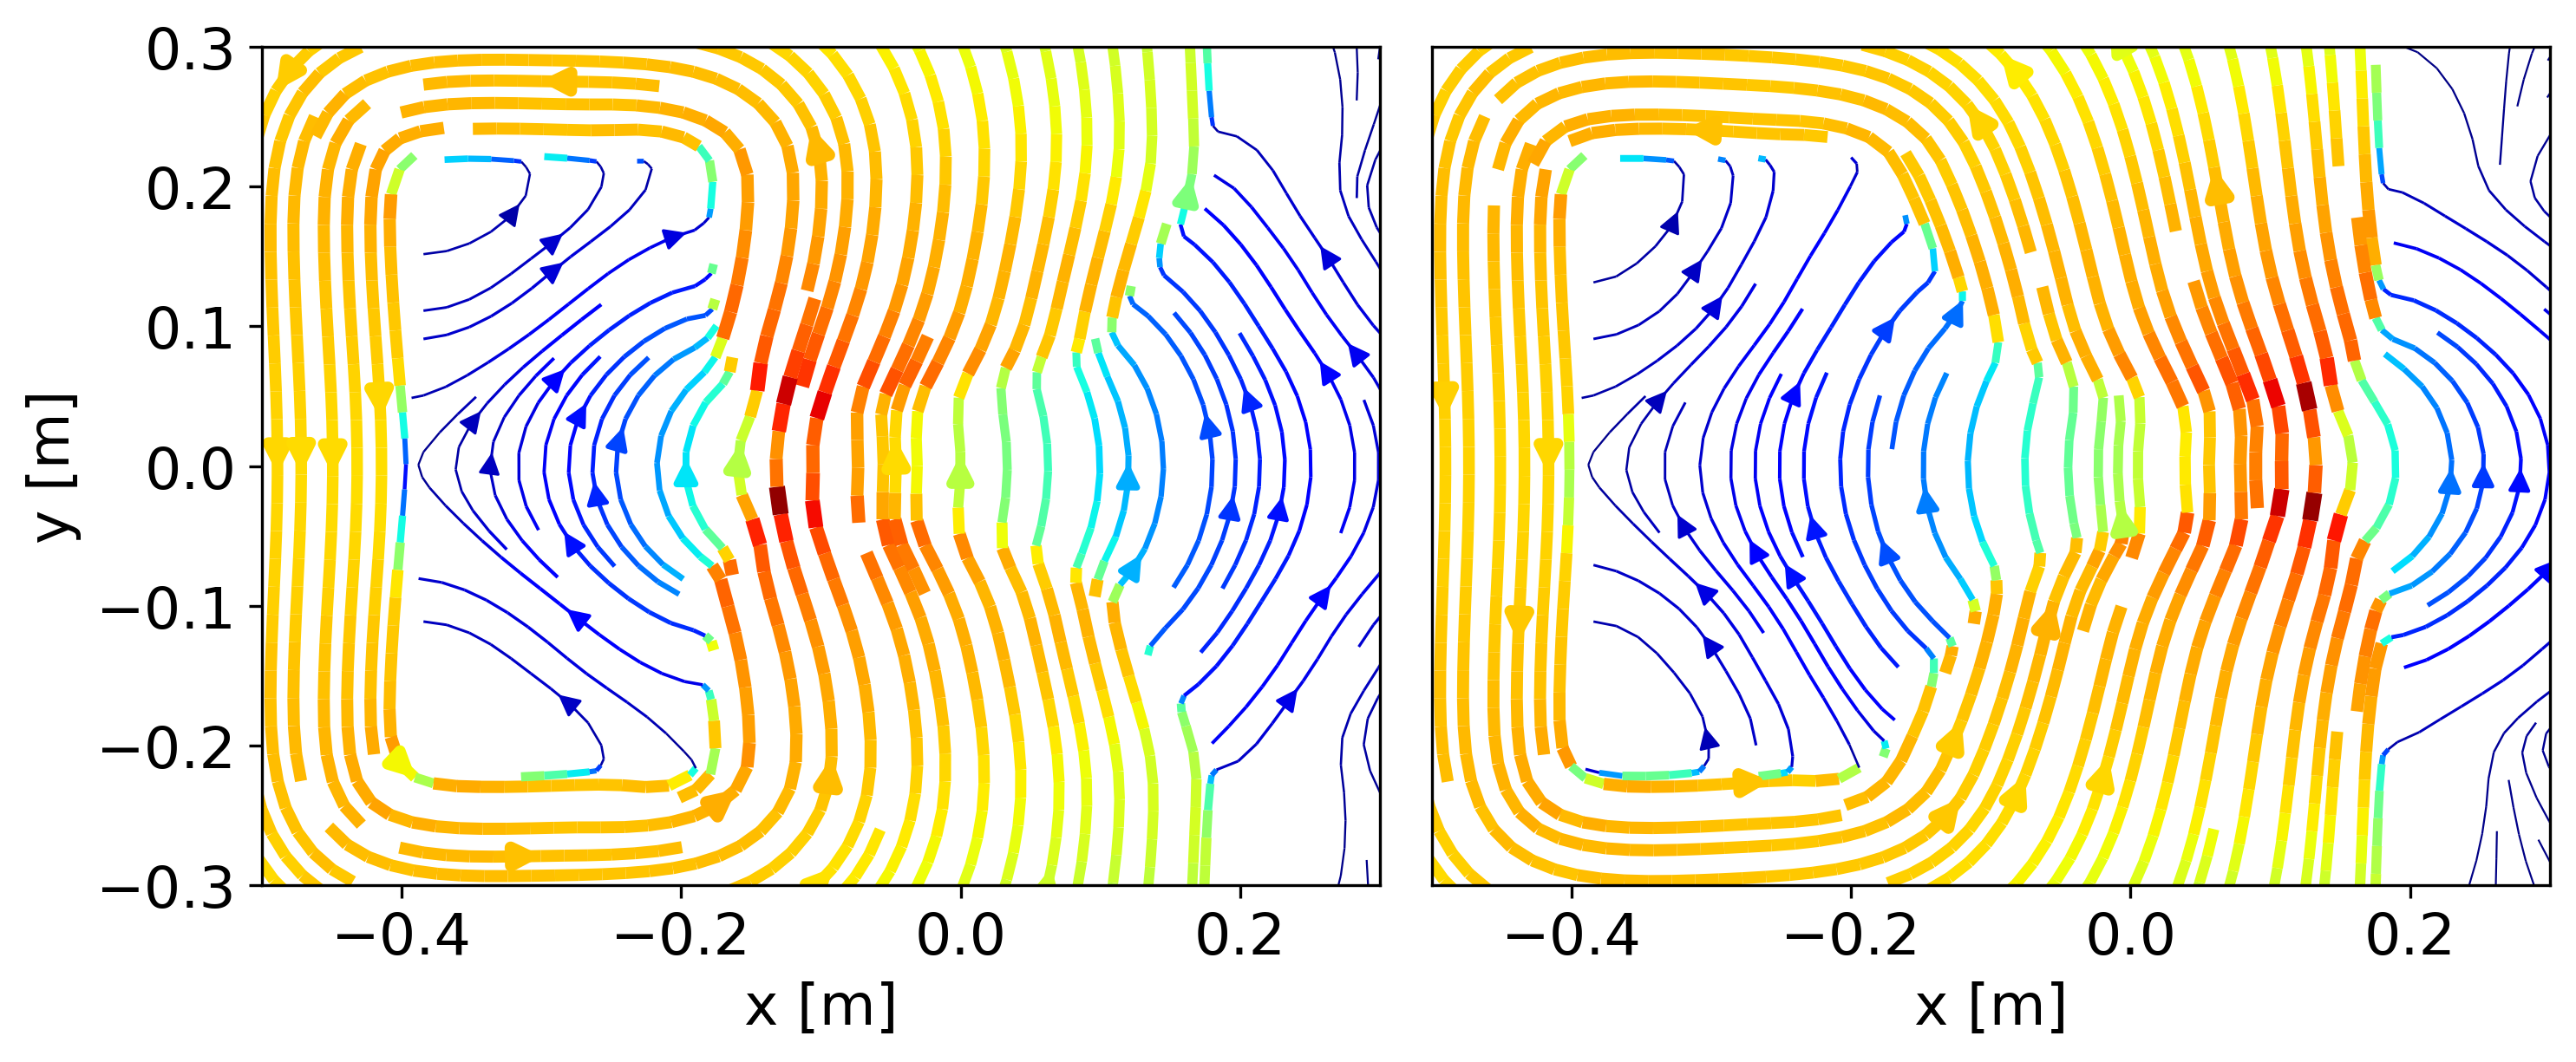
\includegraphics[width=0.7\textwidth]{01_Introduction/images/vector_flow.png}
\caption{Vector flow of an open defocusing block (left) and a closed focusing block (right).}
\label{fig:vector_flow}
\end{figure}

There are four magnets types: R, S, T and U, depending on the arrangement of the half-units (FD or DF) and whether the main coil is on the inside or outside of the ring. Additional coils named the Pole Face Windings (PFW) and Figure-of-eight Loop (F8L) are inserted between the yoke and the vacuum chamber to control the tune and chromaticity. Although the nominal field region of the combined function
magnet extends over a large part of the magnet aperture around the circulating beam orbit, see Fig, \ref{fig:dipole_gradient_components}, the injection and extraction trajectory of the beam travels through strong regions of fringing or stray field. This is a consequence of the PS not being built with straight sections long enough for injection or extraction, forcing the beam to travel through the stray fields of the MUs \cite{risselada_beam_nodate}.
 
\begin{figure}[H]
\centering
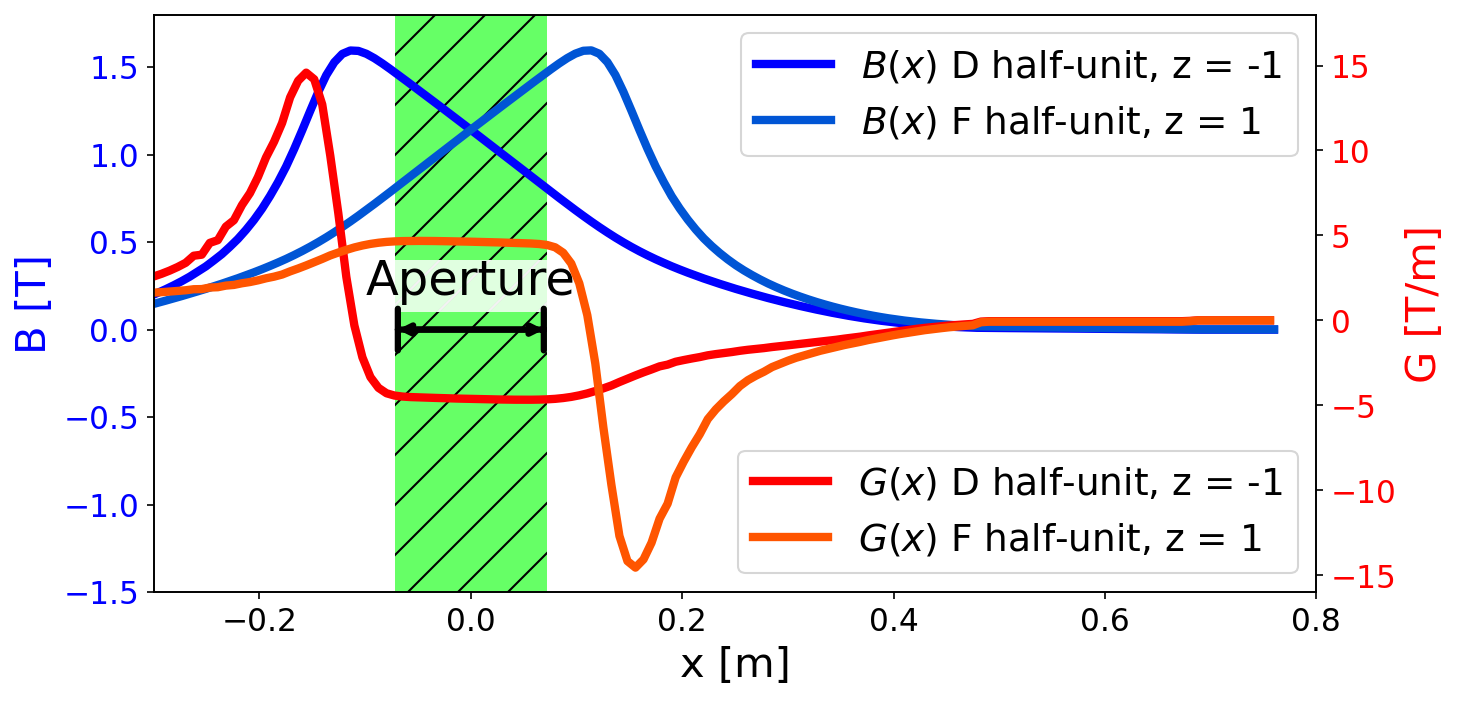
\includegraphics[width=0.7\textwidth]{01_Introduction/images/dipole_gradient_components.png}
\caption{Dipole and gradient component of a PS U-type MU centered in the vertical plane in both half-units at 24 GeV. The green-shaded region of 14.4 cm shows where the gradient is constant to within 5\% of the central and nominal gradient. A width similar to the beam pipe aperture in MU62 of 14.6 cm. Outside this region, the gradient is non-linear and, at its maximum, is almost three-fold higher in amplitude.}
\label{fig:dipole_gradient_components}
\end{figure}

\subsubsection{The OPERA model}

A finite element magnetic model of the PS MU was developed using Cobham's \texttt{Opera-3D}~\cite{noauthor_opera_nodate, anglada_pxmu_hrcwp_nodate} to generate field maps at different energies (different current in the main coils), different PFW, different F8L settings, and for all four magnet types. The model includes the main junction gap of \SI{20}{mm} (a significant source of fringe field) between the two half-units, as well as the mini junctions between open blocks of \SI{9.75}{mm} and \SI{7.75}{mm} between closed blocks. A plane containing the geometry of open and closed yokes is swept in the longitudinal direction, allowing us to maintain a high accuracy of the model and to reduce the computation time. This feature of a single plane also comes with limitations, as it models straight magnets, whilst real magnets have a curvature. The density of the mesh is adjusted so that it has a high resolution in close proximity to the central orbit and at the junctions to capture the fringe fields \cite{anglada_reference_2019}.

An example of a vector field map ($B_x$, $B_y$, $B_z$) in a Cartesian coordinate system ($x$,$y$,$z$) produced by the \texttt{Opera-3D} model is presented in Fig.~\ref{fig:dipole_field}. The transverse displacement of the peak of the vertical dipole field $B_{y}$ along the z-axis corresponds to the switch from one half-unit to the next. The resolution of the field map is high enough to see the mini-junction between the five blocks.

\begin{figure}[!htb]
   \centering
   %trim={<left> <lower> <right> <upper>}
   \includegraphics*[width=0.7\columnwidth, trim={0 2.9cm 0 4.3cm},clip]{01_Introduction/images/dipole_field.png}
   \caption{Dipole field map of a U-type magnet centered in the vertical plane at \SI{24}{GeV}.}
   \label{fig:dipole_field}
\end{figure}

The gradient is calculated from the dipole field component using the following formula:
 
$$ \boldsymbol{G}(x_{j},z) = \frac{\Delta\boldsymbol{B}}{\Delta x} = \frac{\boldsymbol{B}(x_{i+1},z) - \boldsymbol{B}(x_{i},z)}{x_{i+1}-x_{i}} $$
where:
$$ x_{j} = \frac{x_{i+1} + x_{i}}{{2}} $$

\subsubsection{Beam tracking}

Particle tracking through field maps is done using the Boris algorithm that tracks charged particles in EM fields using the discretised equation of motion of the Lorentz force \cite{dutheil_pybttrackersborispy_nodate,qin_why_2013,ripperda_comprehensive_2018}. Field maps were produced for each magnet type at three different energies: injection at \SI{2}{GeV} with \SI{533}{A}, slow extraction to the East Area at \SI{24}{GeV} with \SI{4642}{A}, and extraction to the SPS at \SI{26.4}{GeV} with \SI{5386}{A}. In the following, measurements and tracking studies of injection from the BTP transfer line to the PS and extraction from the PS to the East Area are discussed.

\subsection{Injection via BTP}
As the beam is injected through the BTP transfer line to the PS ring, it passes through the stray fields of the PR.BHT41 T-type MU magnet. The beam traverses mostly through the defocusing half part and feels a non-linear increase in the gradient up to the nominal value in the central orbit; see Fig.~\ref{fig:injection_btp}. Once through MU41, the beam is deflected by the injection septum magnet (PI.SMH42) towards the central orbit. Immediately downstream of the septum, a Secondary Emission Grid (PI.BSG42) is available to measure the position and size of the beam.

\begin{figure}[!htb]
   \centering
   \includegraphics*[width=0.7\columnwidth]{01_Introduction/images/injection_tracking.png}
   \caption{Tracking through MU41 T-type at \SI{2}{GeV}.}
   \label{fig:injection_btp}
\end{figure}

To test the model, measurements of beam position and size on PI.BSG42 were collected as the current provided by the main power supply (POPS) to the MUs was varied. As expected, an increasing current shows that the transverse position of the beam is bent closer towards the inside of the ring by the stronger stray field. Measurements were compared with simulations that tracked a single particle through the \SI{2}{GeV} T-type field map presented in Fig.~\ref{fig:injection_btp_transverse_position}. The tracking simulation overestimates the effect of the stray field because the magnetic model does not yet include the mu-metal shielding wrapped around the injection vacuum pipe. As expected, no deviation was observed in the vertical plane.

\begin{figure}[!htb]
   \centering
   \includegraphics*[width=0.7\columnwidth]{01_Introduction/images/injection_measurement.png}
   \caption{Measurements of the BT3 BTP PS kick response as a function of POPS at PI.BSG42 compared with the OPERA tracking model.}
   \label{fig:injection_btp_transverse_position}
\end{figure}

The current implementation of the stray field in the \mbox{MAD-X}\cite{noauthor_mad_nodate} model is carried out as a sequence of Multipole Field Components (MFC model) expanded along the reference trajectory. A simplified approach with the field components extracted on an injected trajectory assumed as a straight line was compared with the measurements in Fig.~\ref{fig:injection_btp_beam_size}, where the beam size at PI.BSG42 is plotted as a function of the POPS current. We find good agreement in the horizontal plane but a mismatch in the vertical plane. A quadrupole scan was performed on PI.BSG42 and an analysis will tell us whether this is the result of incorrect initial parameters. Similar MFC models for injection and extraction will be created using a Taylor series of the multipole components of the magnetic field about the curved trajectory of the reference particle.

\begin{figure}[!htb]
   \centering
   \includegraphics*[width=0.7\columnwidth]{01_Introduction/images/injection_measurement_beam_size.png}
   \caption{Measurements of the BT3 BTP PS beam size as a function of POPS at PI.BSG42 compared with the MFC model.}
   \label{fig:injection_btp_beam_size}
\end{figure}

\subsection{Extraction to the East Area}
The beam extracted to the East Area is significantly affected by stray fields in multiple main units because the slow extracted trajectory at high energy has a much shallower angle than at injection. As presented in Fig.~\ref{fig:stray field gradients}, the difference in the gradient of MU62 is striking in that the sign of the gradient flips and triples in amplitude. As a result, an increase in the horizontal beam size is expected at the exit of MU62. It is not understood why this magnet was not shimmed in the past to help reduce the effect of the stray field (perhaps because they would significantly impact the central orbit \cite{Zickler:private}), but it is undoubtedly the cause of the optics discrepancy observed during commissioning of the East Area transfer lines in 2021 \cite{huschauer:ipac22-mopost006}.

\begin{figure}[!htb]
   \centering
   \includegraphics*[width=0.7\columnwidth]{01_Introduction/images/gradient_stray_field.png}
   \caption{Gradient seen by the slow extracted beam in the stray field of the few last MUs's focusing half-unit.}
   \label{fig:stray field gradients}
\end{figure}

\subsubsection{Magnetic shims}

To counteract stray fields, magnetic shims are installed in MU16 (fast extraction to SPS) and MU63 (slow extraction to East Area) to homogenise the field by shielding the ejected beam from the non-linear fringe field \cite{zickler_influence_nodate}. In MU16, the shims have different radial positions for each of the five different shims, while in MU63, the vacuum pipe is covered with a constant rectangular shim. In MU62, no shims are installed, where the model predicts the most important stray field effect. In the next step, the shim geometry will be incorporated into the \texttt{OPERA-3D} model, which will significantly increase the computation time of the finite element solver due to the increased complexity of the geometries, but will allow for a more accurate representation of the actual stray fields.

\subsubsection{Measurement of the extracted beam parameters}

Quadrupole scans have been performed to reconstruct the beam parameters in the East Area extraction line. The beam size was measured with Beam instrumentation - TV (BTV) screens as the strength of one or multiple quadrupoles was varied. The initial parameters can be determined empirically by fitting them to a MAD-X simulation against the measurements. BTVs are not ideal instruments for performing these measurements; they saturate at the extraction intensities, and the signal must be fitted with care. Filter wheels have been installed to reduce saturation, allowing for more accurate initial parameter measurement. In addition, a dispersion measurement will be performed to reduce the degrees of freedom of fit.
Kick response measurements have also been carried out. Future studies will compare the initial parameters measured with those predicted by tracking through the field maps in MAD-X.

%\textbf{State clearly the efforts we are going to here to measure the beam parameters that come out of the machine and through the stray fields. State the quad scan technique and challenges with lack of instrumentation but that work continues with BTVs and additional of filter wheels for a comparison with simulation}





\subsection{Previous studies done on the stray fields}

\subsection{Geometry, where do you expect to find stray fields (at injection and extraction F16 and F61)}

\subsection{Shims (no shims in MU62 and shims in MU63)}

%%%%%%%%%%%%%%%%%%%%%%%%%%%%%%
%%%%%% Simulation %%%%%%%%%%%%
%%%%%%%%%%%%%%%%%%%%%%%%%%%%%%

\section{Simulation}
\label{section:simulation}

\subsection{MAD-X}

\subsection{OPERA model of the MU (I can cite here the IPAC paper)}

\subsection{Explain that it defocuses in H and focuses in V}

\cite{johnson_beam_2022}

\subsection{Kick response (maybe I need more data and MD for this or simply repeat the measurements)}

\subsection{Injection BTP MD}

\subsection{BTP stray elements}

The BTP line has an old model (prior to 2021) that is composed of 233 thin multipole inserted at the end of the transfer line. The model can be accessed via the following links:

\begin{itemize}
    \item \href{https://gitlab.cern.ch/acc-models/acc-models-tls/-/blob/2021/psb_extraction/btp/BTP.ele}{BTP.ele}
    \item \href{https://gitlab.cern.ch/acc-models/acc-models-tls/-/blob/2021/psb_extraction/btp/BTP.seq}{BTP.seq}
\end{itemize}



\subsection{Theory}

The magnetic field \( B_y \) can be expressed as:

\[
B_{y}(x,y) = B_{0} + B_{1}x + B_{2}\frac{1}{2}(x^{2}-y^{2}) + B_{3}\frac{1}{6}(x^{3}-3xy^{2})
\]

where the coefficients \( B_i \) are given by:

\[
B_{i} = K_{i}B\rho
\]

In the old BTP model, the coefficients \( K_{0}, K_{1}, K_{2}, \) and \( K_{3} \) are used.

The relationship for \( K_{0} \) is:

\[
K_{0}L = \frac{B_{0}L}{B\rho}
\]

where 

\[
L = \frac{\text{totalLength}}{\# \text{ elements}}
\]

To extract the pure \( K_{0} \), we divide by \( L \):

\[
K_{0} = \frac{B_{0}}{B\rho}
\]

For tracking, we obtain the field components and divide by \( B\rho \):

\[
B_{0} = K_{0}B\rho
\]

\[
K_{0} = \frac{B_{0}}{B\rho}
\]

The \( K_{1} \) coefficient is computed using two tracks and the relationship:

\[
K_{1} = \frac{\frac{\Delta B_{y}}{\Delta x}}{B\rho}
\]

The \( K_{0}L \) component as a function of \( s \) is shown as follows:

\begin{figure}[H]
\centering
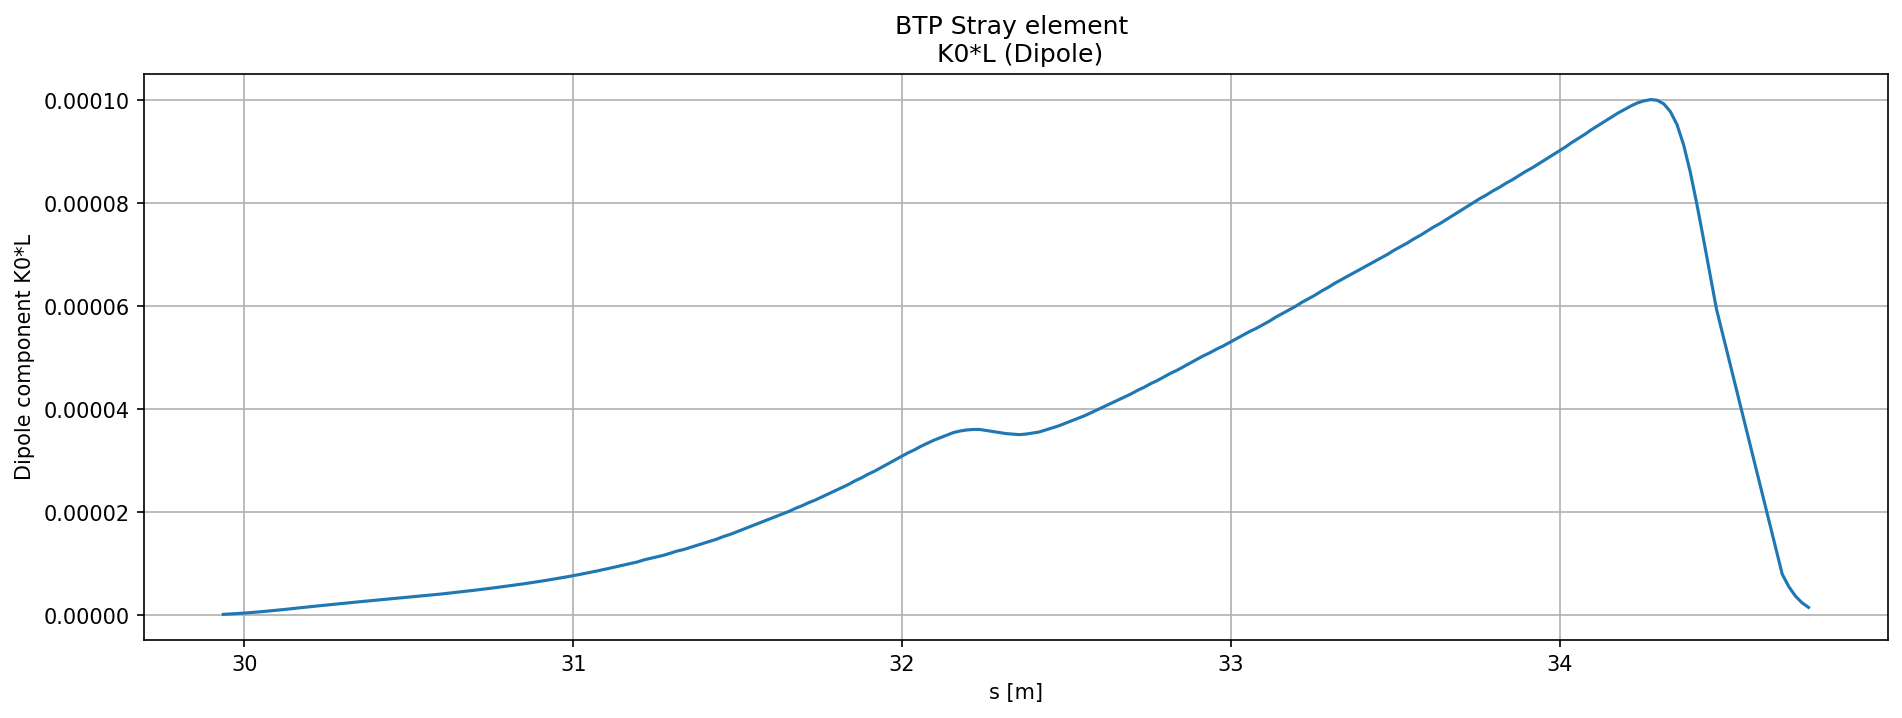
\includegraphics[width=1.0\textwidth]{02_Simulation/images/BTP_old_model_stray.png}
\caption{BTP Stray element old model.}
\label{fig:transfer_matrix_1}
\end{figure}


A goal is to create a multi-component model similar to the old BTP model, first on the BTP line to compare with the old model and then to expand on different injection and extraction that passes through stray fields. The first step is launch particles on the reference track, track them in the stray field magnetic field and probe the B-field perpendicular to the track. Then a 4rd order polynomial is fit for everything position along the injection line, i.e. along different z in meters.

\begin{figure}[H]
\centering
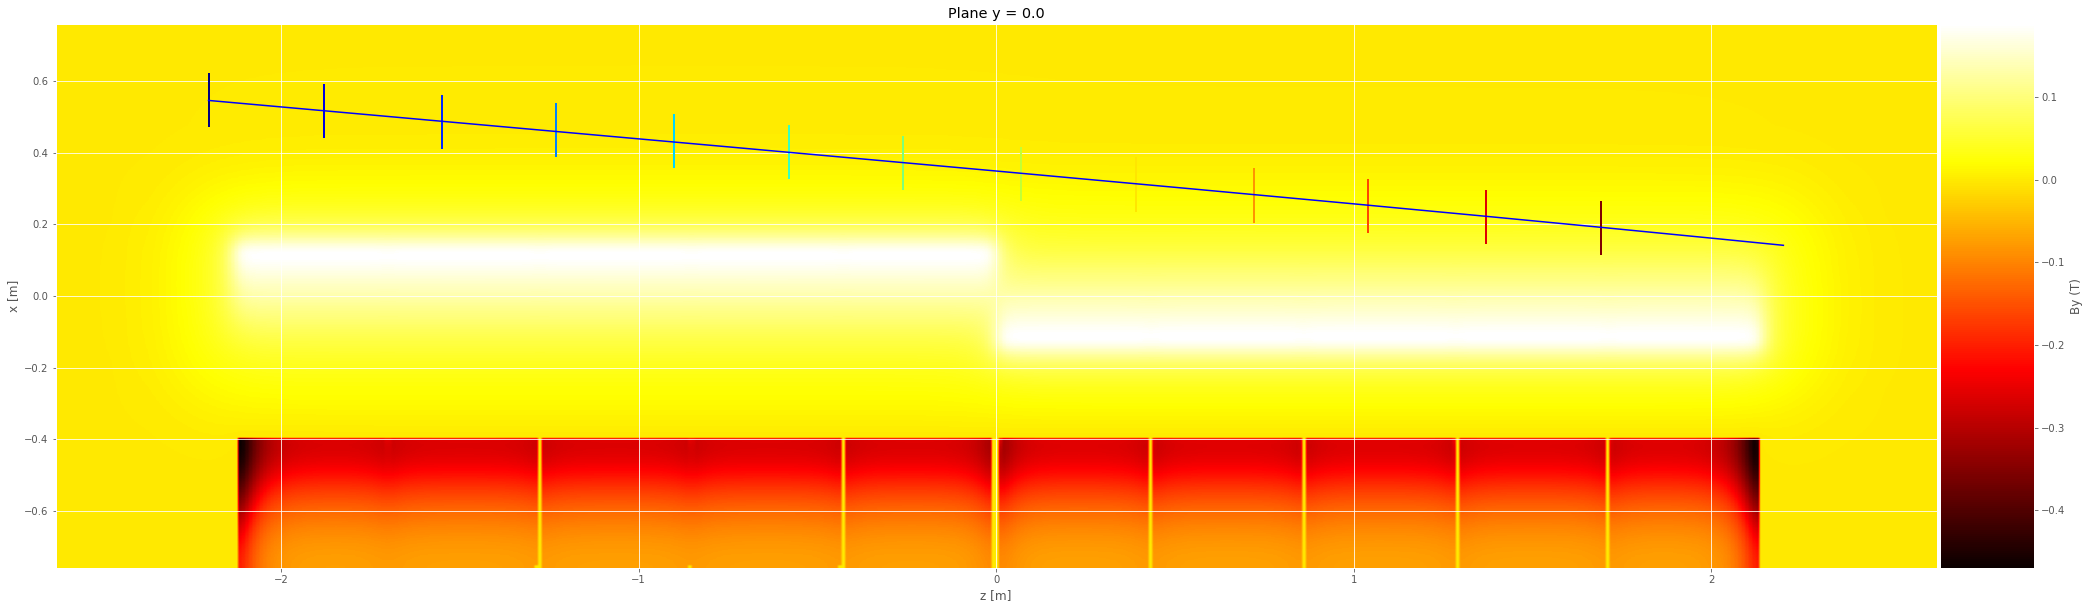
\includegraphics[width=1.0\textwidth]{02_Simulation/images/MCP_track.png}
\caption{Tracking through the MCP injection.}
\label{fig:mcp_track}
\end{figure}

\begin{figure}[H]
\centering
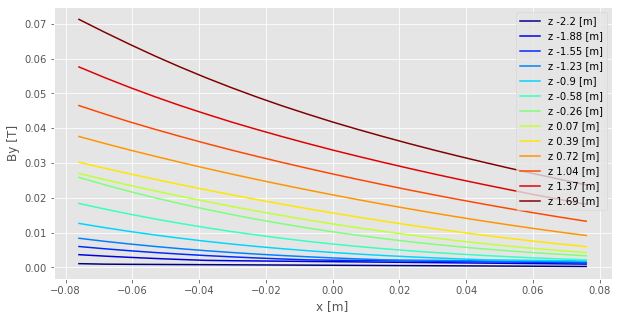
\includegraphics[width=1.0\textwidth]{02_Simulation/images/MCP_track_2.png}
\caption{Probing the B-field tranversly to the injection track.}
\label{fig:mcp_track}
\end{figure}



\begin{figure}[H]
\centering
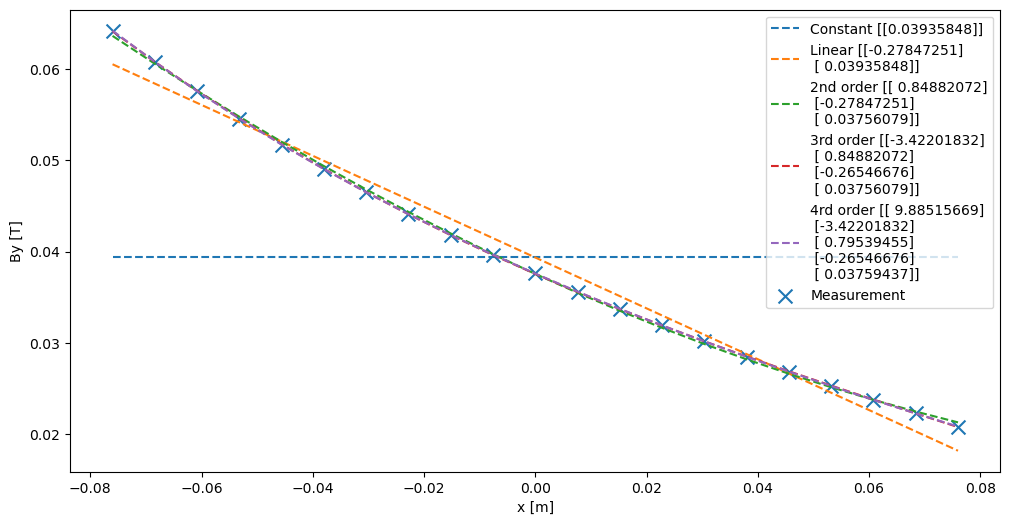
\includegraphics[width=1.0\textwidth]{02_Simulation/images/fit_of_bfield.png}
\caption{.}
\label{fig:fit_bfield}
\end{figure}

\begin{figure}[H]
\centering
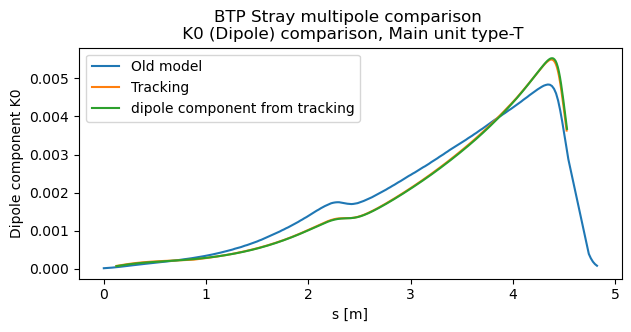
\includegraphics[width=0.7\textwidth]{02_Simulation/images/mcp_dipole.png}
\caption{BTP Stray multipole comparison, K0 (Dipole) comparison, main unit type-T}
\label{fig:mcp_dipole}
\end{figure}

\begin{figure}[H]
\centering
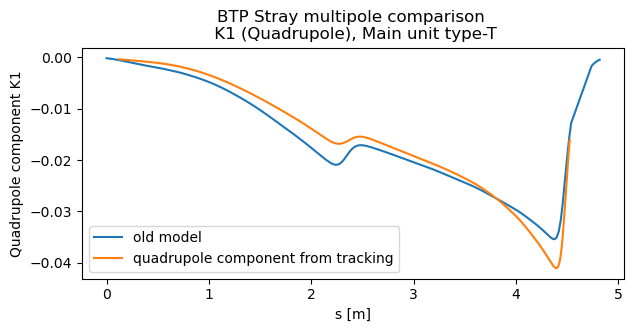
\includegraphics[width=0.7\textwidth]{02_Simulation/images/mcp_quadrupole.png}
\caption{BTP Stray multipole comparison, K1 (Quadrupole) comparison, main unit type-T}
\label{fig:mcp_quadrupole}
\end{figure}

\begin{figure}[H]
\centering
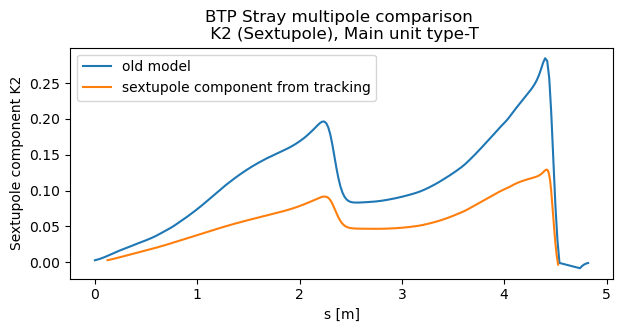
\includegraphics[width=0.7\textwidth]{02_Simulation/images/mcp_sextupole.png}
\caption{BTP Stray multipole comparison, K2 (Sextupole) comparison, main unit type-T}
\label{fig:mcp_sextupole}
\end{figure}

\begin{figure}[H]
\centering
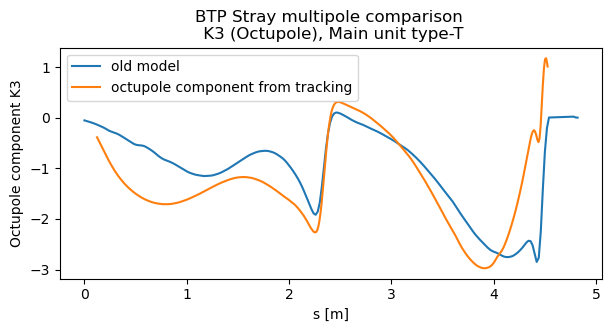
\includegraphics[width=0.7\textwidth]{02_Simulation/images/mcp_octupoles.png}
\caption{BTP Stray multipole comparison, K3 (Octupoles) comparison, main unit type-T}
\label{fig:mcp_quadrupole}
\end{figure}


The code creates MCP models correctly along the s dimension (along the particles track) and transverse along the bend track. For small angles, the difference in dipole component along z or s can be neglected.

\subsection{Multipole field component in MU62}

This section will talk about the multiple field component inside the MU62 main unit which is the magnet that the beam crosses through for the extraction to the East Area.

The following \href{https://gitlab.cern.ch/eljohnso/acc-models-tls-eliott-fork/-/blob/EliottBranch/ps_extraction/east-fast-extraction/mfc_mu62.ipynb}{Notebook: MFC MU62} was used to create the MFC in MU62 using a \SI{24}{\giga\electronvolt\per\clight} beam. Figure \ref{fig:track_mu62} shows the particle track through the stray field of MU62. The initial launching coordinate of the reference particle were \si{0.132}{m} and \si{0.0139}{rad}. The field was probed transversely at discrete s-steps along the particle trajectory inside the vacuum pipe. The vacuum pipe aperture has a total width of \si{70}{mm}. We run a loop for each point in the track we save the $B_{y}$ field perpendicularly to the track  and run a polynomial fit of third order on By as a function of $x_{\perp}$

$$ \alpha = - tan^{-1}\left(\frac{ x_{i}-x_{i-1} } {z_{i}-z_{i-1}} \right)$$

$$ B_{y} = \begin{bmatrix}  
x_{center} + x_{offset}\cdot cos(\alpha_{deflection}) \\  
0 \\
z_{center} + x_{offset}\cdot sin(\alpha_{deflection})
\end{bmatrix} $$



\begin{figure}[H]
\centering
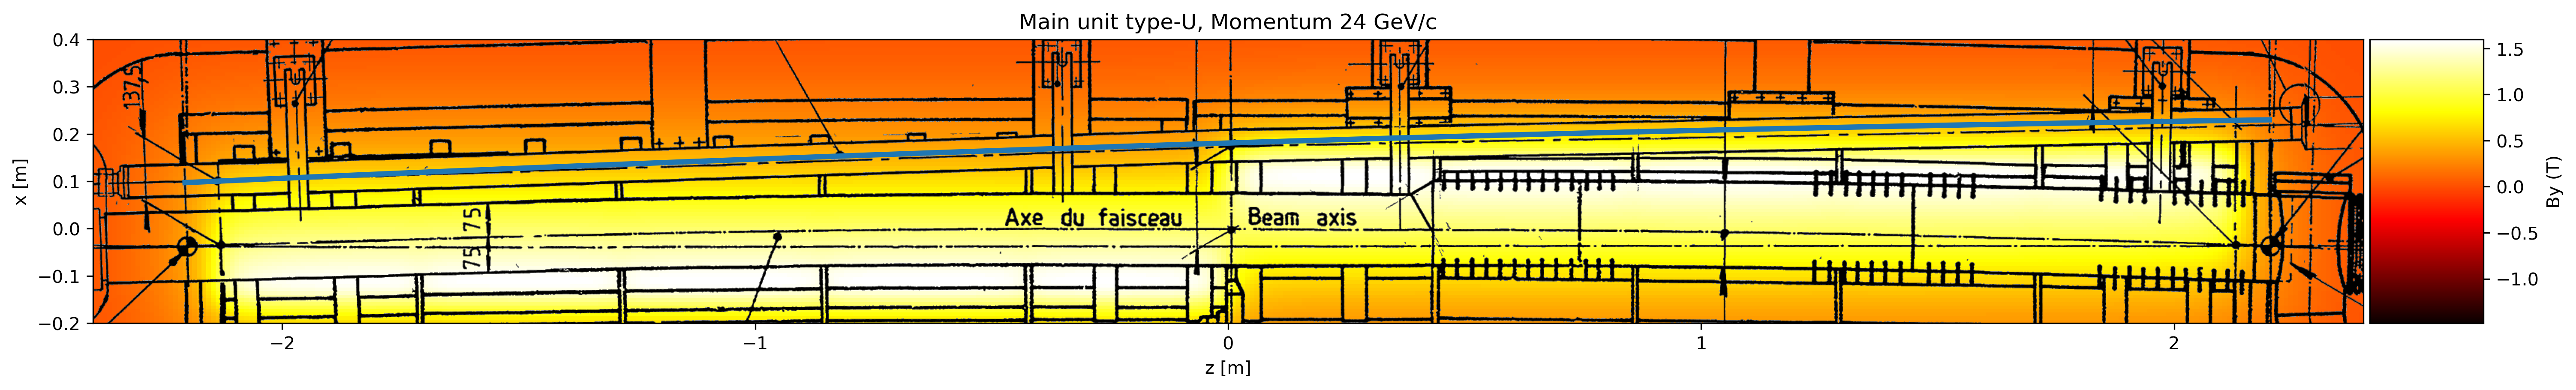
\includegraphics[width=1.0\textwidth]{02_Simulation/images/track_mu62.png}
\caption{Tracking of the proton beam in MU62}
\label{fig:track_mu62}
\end{figure}

\begin{figure}[H]
\centering
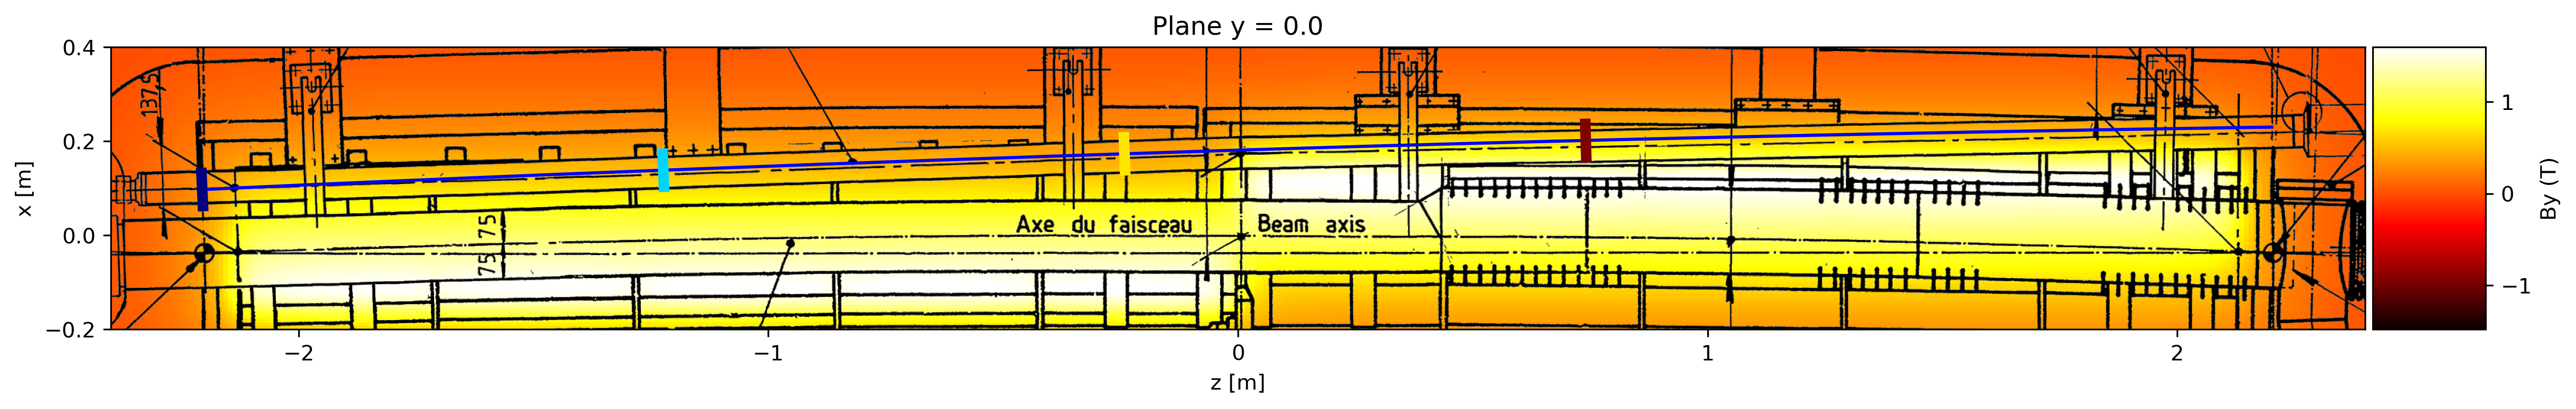
\includegraphics[width=1.0\textwidth]{02_Simulation/images/track_mu62_2.png}
\caption{Tracking of the proton beam in MU62 with example location of MFC sampling}
\label{fig:track_mu62_2}
\end{figure}

\begin{figure}[H]
\centering
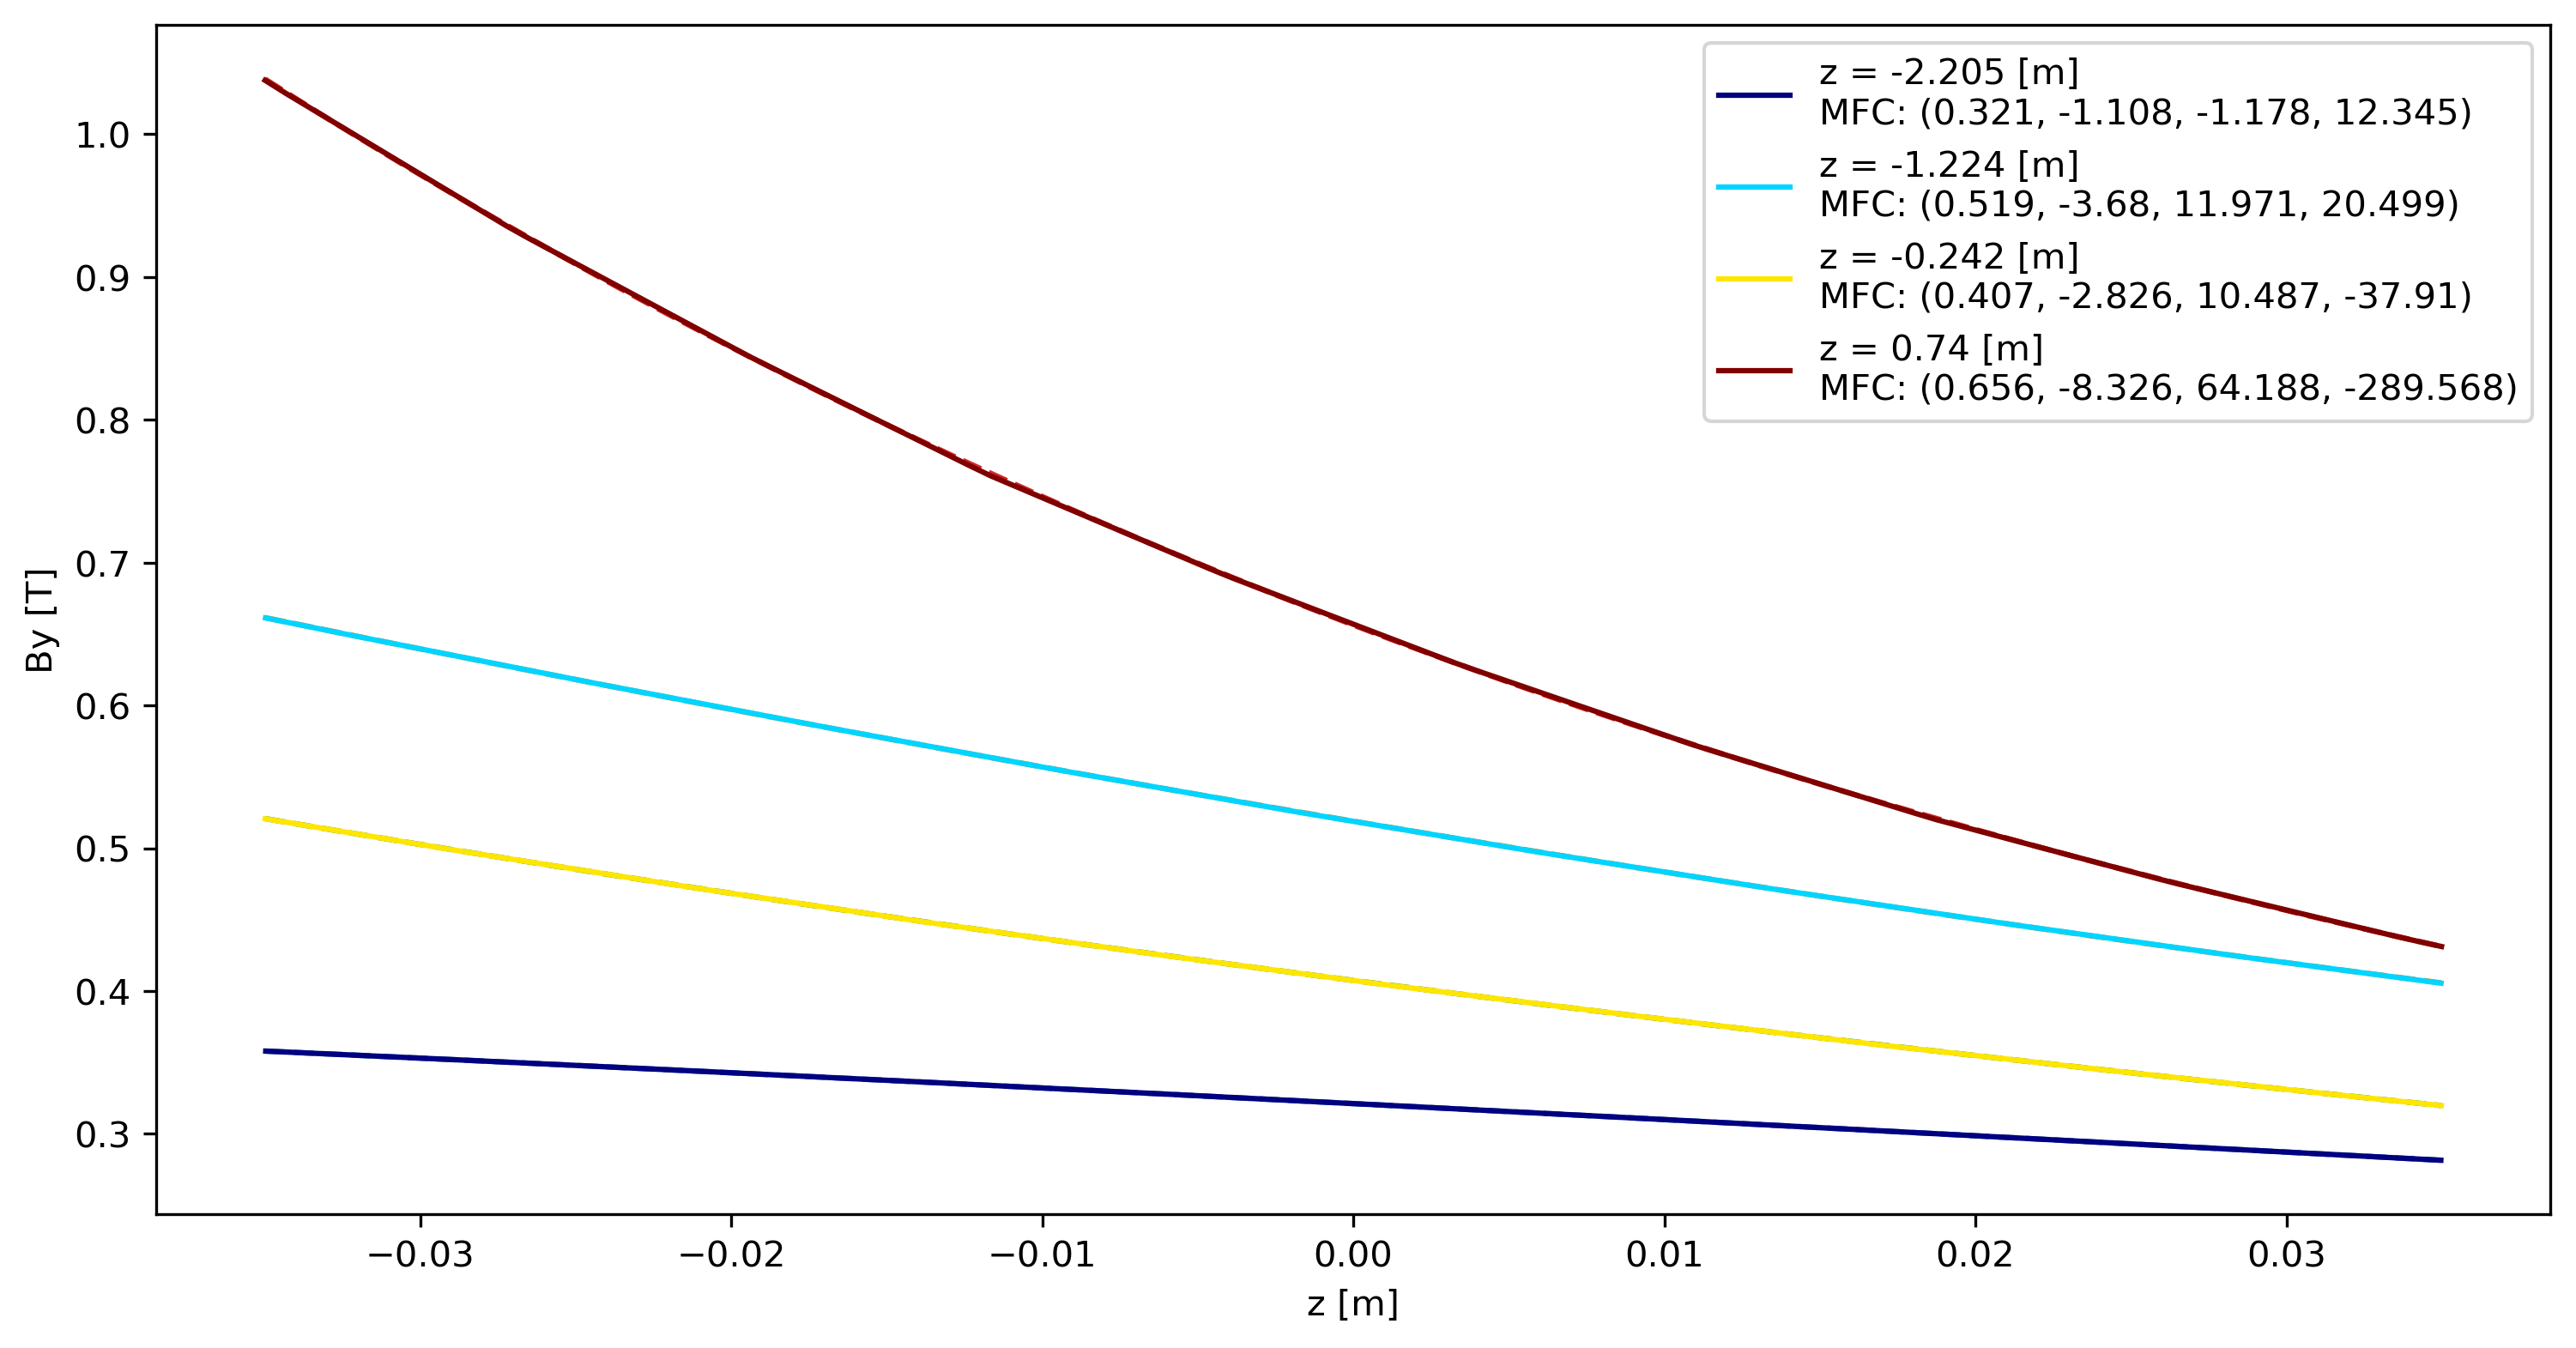
\includegraphics[width=0.7\textwidth]{02_Simulation/images/track_mu62_2_mfc.png}
\caption{Tracking of the proton beam in MU62 MFC transverse dipoles component.\textcolor{red}{The x-label should be $x_{T}$} }
\label{fig:track_mu62_2_mfc}
\end{figure}

Full tracking with along the beam line gives us the following MFC shown.

\begin{figure}[H]
\centering
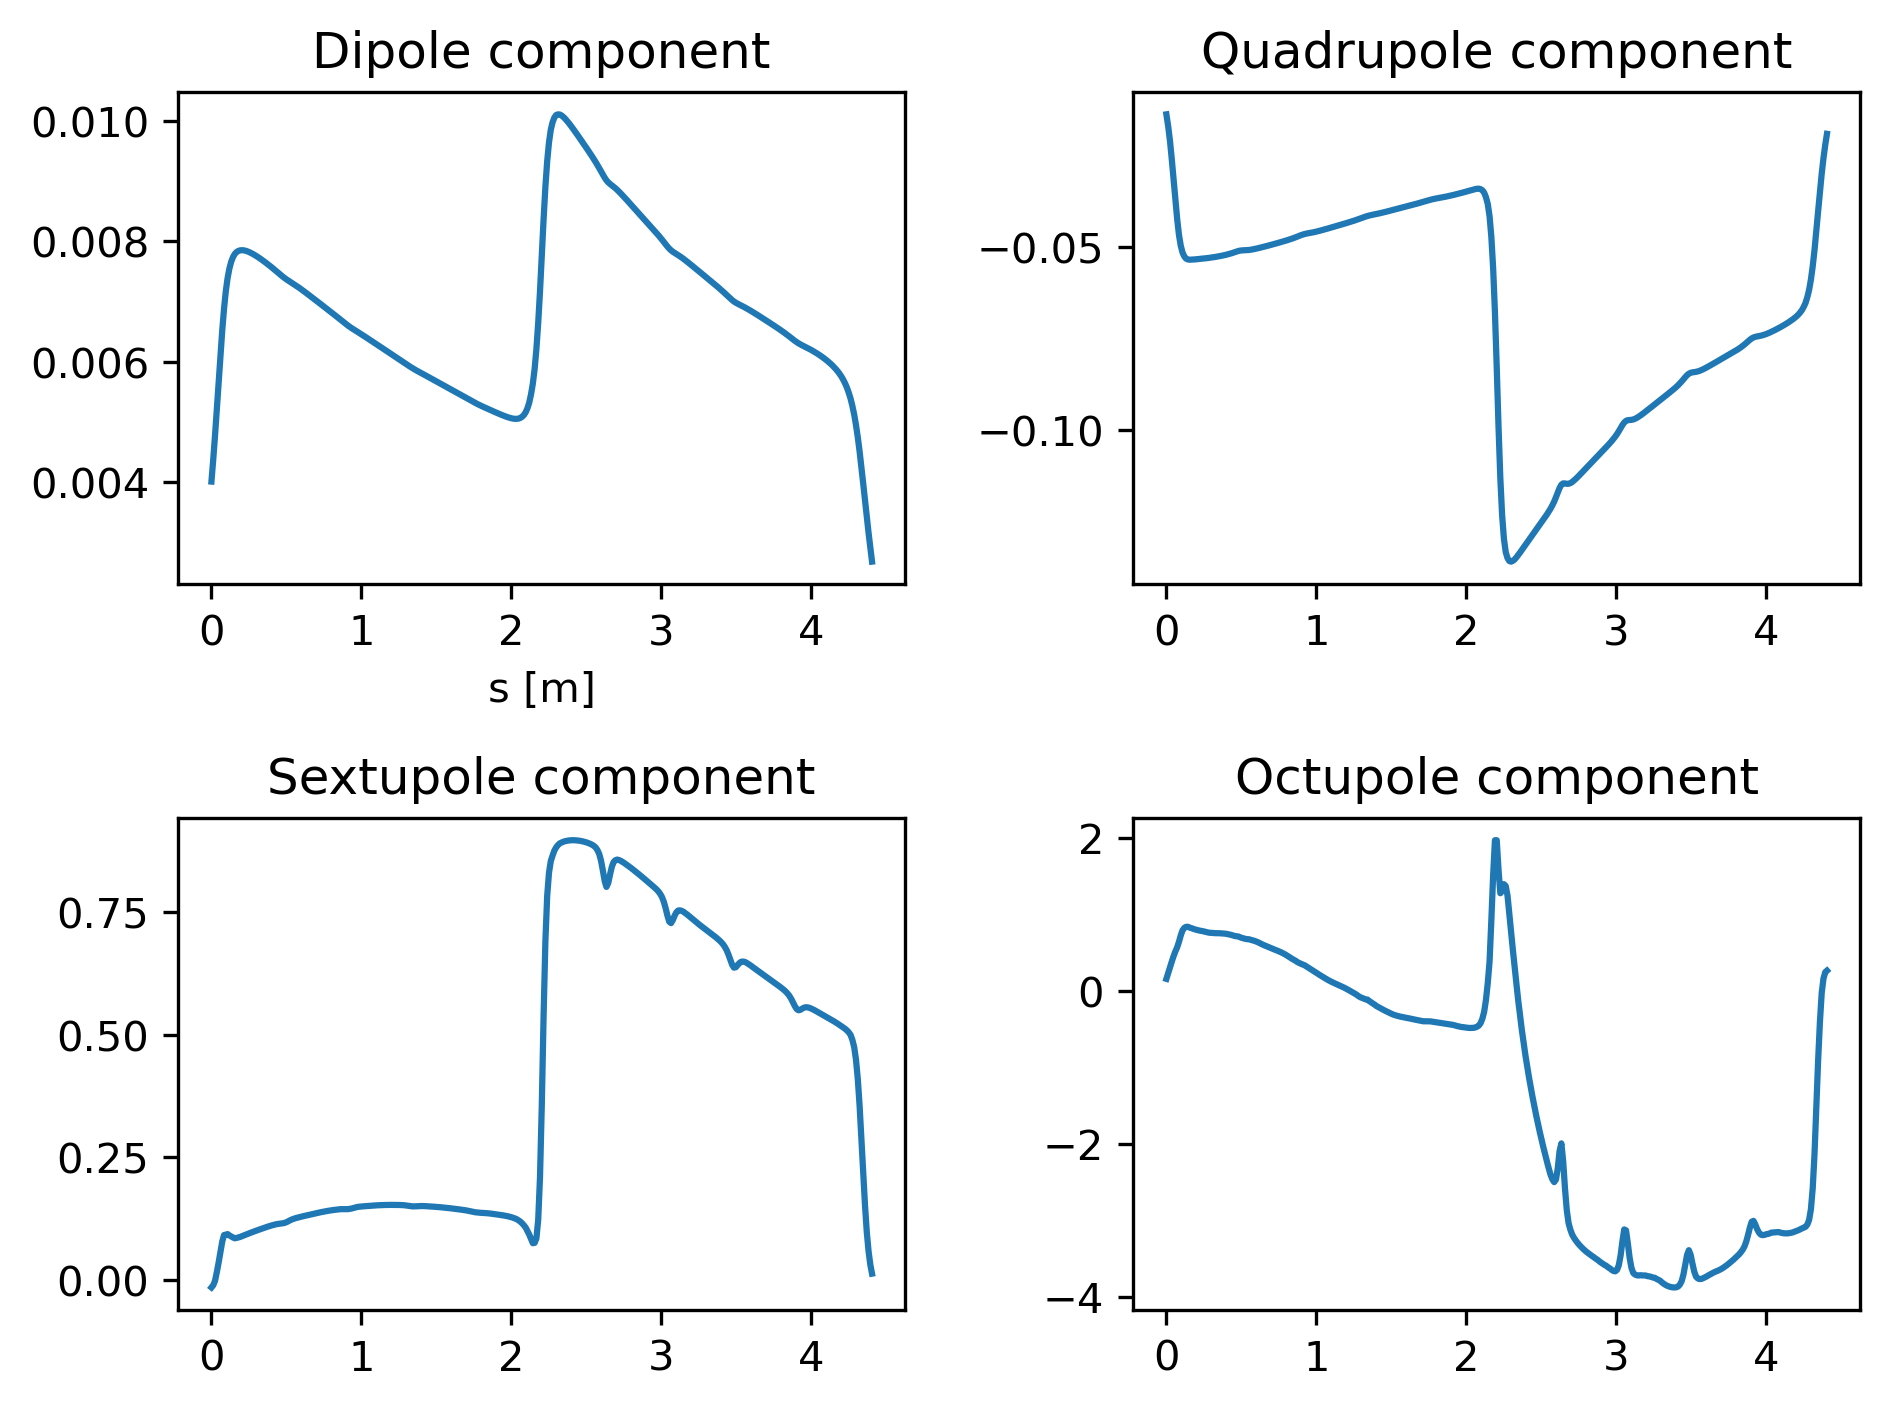
\includegraphics[width=0.7\textwidth]{02_Simulation/images/mfc_mu62.png}
\caption{MFC in MU62.}
\label{fig:mfc_mu62}
\end{figure}

Theses MFC components can be exported to a file to be used in MAD-X. The format for the \texttt{.ele} file is as follows:

\begin{lstlisting}
stray1 : multipole, knl:={2.11E-07,-3.11E-06,5.25E-05,-0.001056026};
stray2 : multipole, knl:={2.78E-07,-4.03E-06,6.74E-05,-0.001303161};
stray3 : multipole, knl:={3.54E-07,-5.09E-06,8.47E-05,-0.001548501};
\end{lstlisting}

When you export the multipole component you need to multiply by the length of the multipole element i.e.:

\[
\frac{L_{\text{Total}}}{l_{\text{element}}}
\]

The format for the \texttt{.seq} file is as follows:

\begin{lstlisting}
stray1, at = 29.9366067;
stray2, at = 29.9566067;
stray3, at = 29.9766067;
\end{lstlisting}

\subsection{Initial condition in F61D}

The MFC model was added to the F61D transfer line in MAD-X, see Fig. \ref{fig:f61d_with_stray}. The F61D with stray field line \href{https://gitlab.cern.ch/eljohnso/acc-models-tls-eliott-fork/-/blob/c6cbcafacca274000d2bfc501f39cf711375de90/ps_extraction/east-fast-extraction/f61d_with_stray/F61D_with_stray.ipynb}{script} has the stray field element of the MU62 magnet decomposed into multipole and can be found at \href{https://gitlab.cern.ch/eljohnso/acc-models-tls-eliott-fork/-/blob/c6cbcafacca274000d2bfc501f39cf711375de90/ps_extraction/east-fast-extraction/f61d_with_stray/strayMU62.ele}{strayMU62.ele} and \href{https://gitlab.cern.ch/eljohnso/acc-models-tls-eliott-fork/-/blob/c6cbcafacca274000d2bfc501f39cf711375de90/ps_extraction/east-fast-extraction/f61d_with_stray/strayMU62.seq}{strayMU62.seq}.

\begin{figure}[H]
\centering
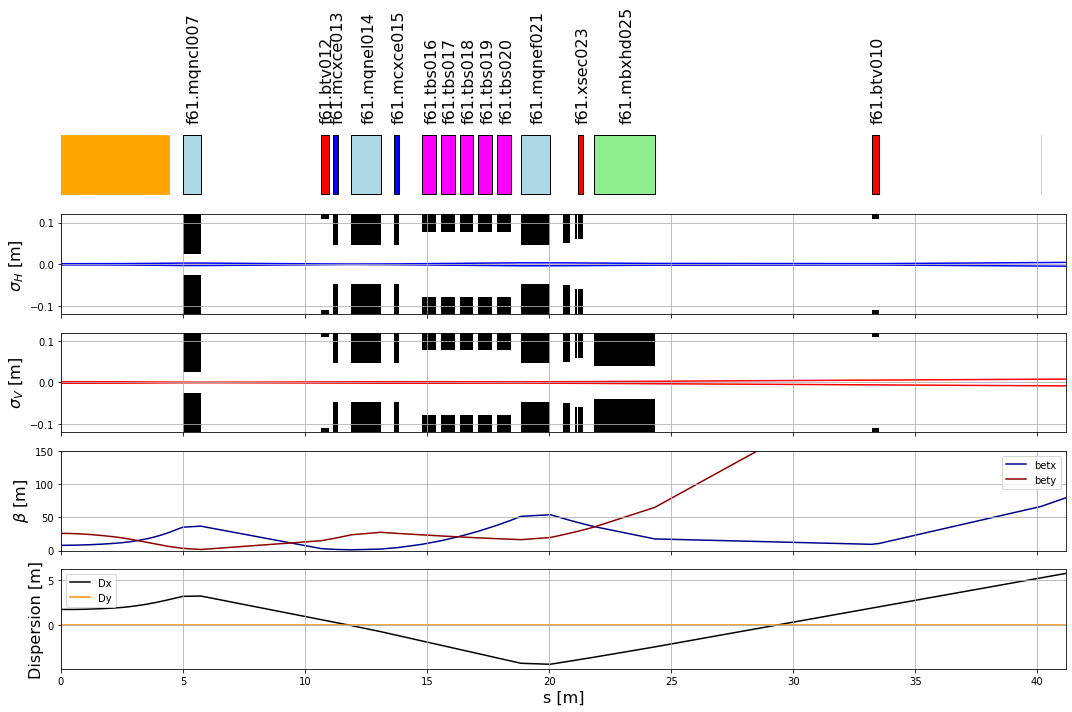
\includegraphics[width=1.0\textwidth]{02_Simulation/images/F61D_with_stray.png}
\caption{F61D with stray field multipole of MU62. The orange rectangle in the synoptic represents the multipole component of the stray field.}
\label{fig:f61d_with_stray}
\end{figure}


The initial condition of the F61D transfer line were found using the twiss parameters from the PS Ring slow extraction \href{https://gitlab.cern.ch/eljohnso/acc-models-tls-eliott-fork/-/blob/EliottBranch/ps_extraction/east-fast-extraction/Check%20scripts/slow_extraction_trajectory_maptrack_inital_conditions.ipynb}{script}. The beam enveloppe was extracted using a pycollimate simulation and retrieving the four particles marking the edge of the extracted separatrix, see Fig. \ref{fig:init_pycollimate}. The tune of the PS was match to be on resonance and the chromaticity match to measurement from 12.11.2021 (Qxp=-1.239, Qyp=0.242). These four particles were tracked during their last turn before being extracted in the PS with the electrostatic septum and the magnetic septa on. The strength of the electrostatic septum (SEH23) was determined by applying a voltage of \SI{-177}{\kilo\volt} across a gap of \SI{15.11}{\milli\metre}, resulting in an electric field of \SI{11.708}{\mega\volt\per\metre}. Given an effective length of \SI{0.8}{\metre}, the resulting strength was calculated as $\theta_{SEH23} = \arctan \left( \frac{|\mathbf{E}| \cdot \text{effective length}}{p \cdot \beta \cdot 10^9} \right)$, and incorporated into the MAD-X input as $kPESEH23$.

For the magnetic septa, the strength of SMH57 was derived from a current of \SI{9120}{\ampere} (measured on 12.11.21), scaled from codilog data to obtain a strength of $\theta_{SMH57} = \frac{\text{current} \cdot 0.378}{9871 \cdot \mathbf{B} \rho}$, which was input into MAD-X as $kPESMH57$. Similarly, SMH61 had a measured current of \SI{1170}{\ampere} (measured on 12.11.21), with a strength calculated as $\theta_{SMH61} = \frac{\text{current} \cdot 0.247}{2350 \cdot \mathbf{B} \rho}$, and input into MAD-X as $kPESMH61$.



\begin{figure}[H]
\centering
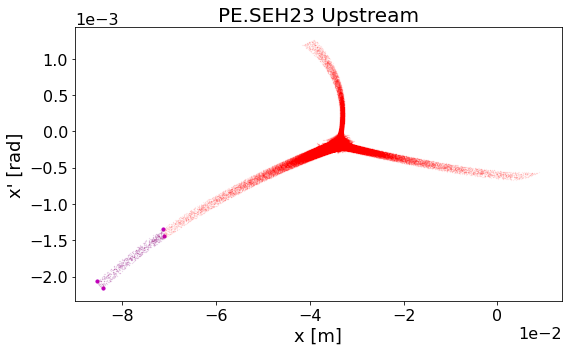
\includegraphics[width=0.7\textwidth]{02_Simulation/images/init_pycollimate.png}
\caption{Distribution of particles in the PS and the four particles at the extremity of the separatrix used as beam envelope.}
\label{fig:init_pycollimate}
\end{figure}

Figure \ref{fig:beam_envelope} shows the envelope of the slow extraced beam from the PS to the East Area. This simulation was used to calculate the initial conditions before entering the stray fields of MU62.


\begin{figure}[H]
\centering
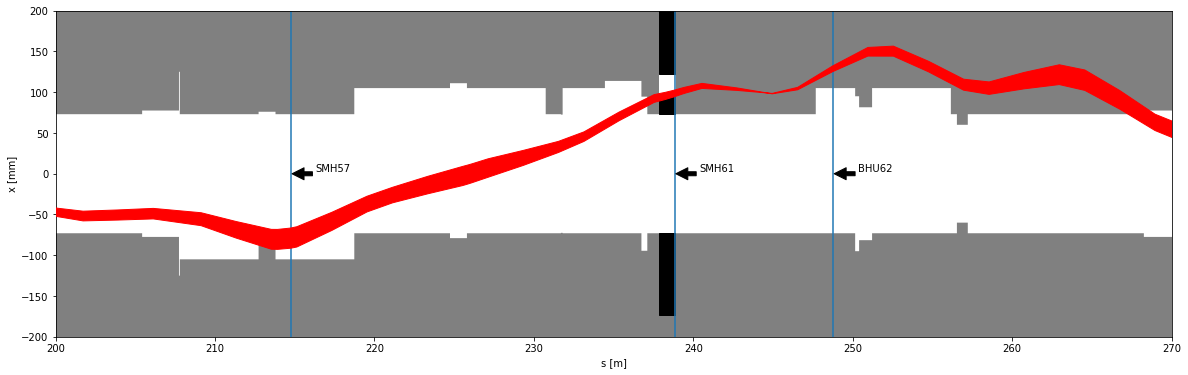
\includegraphics[width=1.0\textwidth]{02_Simulation/images/beam_envelope.png}
\caption{Beam envelope through SMH57, SMH61 and at the entrance of MU62.}
\label{fig:beam_envelope}
\end{figure}

\begin{table}[ht]
    \centering
    \caption{Initial condition upstream of the MU62 magnet}
    \begin{tabular}{l c}
        \hline
        \textbf{Twiss Parameter} & \textbf{Value} \\
        \hline
        $\beta_{x0}$ & 7.48 \\
        $\beta_{y0}$ & 26.14 \\
        $\alpha_{x0}$ & 0.0021 \\
        $\alpha_{y0}$ & 0.0591 \\
        $D_{x0}$ & 1.428 \\
        $D_{y0}$ & 0.0 \\
        $D'_{x0}$ & -0.021 \\
        $D'_{y0}$ & 0.0 \\
        \hline
    \end{tabular}
    \label{tab:twiss_parameters}
\end{table}

\begin{table}[ht]
    \centering
    \caption{Comparison of Simulated and Measured Twiss Parameters after the MU62 stray fields.}
    \begin{tabular}{l c c}
        \hline
        \textbf{Twiss Parameter} & \textbf{Simulated} & \textbf{Measured} \\
        \hline
        $\beta_{x0}$ & 35 & 154 \\
        $\beta_{y0}$ & 3.4 & 5.2 \\
        $\alpha_{x0}$ & -7.4 & -37 \\
        $\alpha_{y0}$ & 2.1 & 0.25 \\
        $D_{x0}$ & 3.2 & 0.13 \\
        $D_{y0}$ & 0 & 0 \\
        $D'_{x0}$ & 0.63 & 0.02 \\
        $D'_{y0}$ & 0 & 0 \\
        \hline
    \end{tabular}
    \label{tab:twiss_comparison}
\end{table}

The comparison of the simulated and measured Twiss parameters after the MU62 stray fields reveals significant discrepancies. The simulated values for $\beta_{x0}$, $\alpha_{x0}$, and $D_{x0}$ show considerable deviations from the measured data, with the simulated $\beta_{x0}$ and $\alpha_{x0}$ being notably lower than the measured values. These differences suggest that the simulation model does not accurately capture the conditions observed in the empirical measurements. Further investigation is required to identify the underlying causes of these discrepancies and to improve the accuracy of the simulation model. Adjustments to the model parameters or the inclusion of additional physical effects might be necessary to achieve better alignment between simulation and measurement.

\subsection{Stitched model}

The slow extraction cannot be transported with a twiss, you need to perform tracking. The distribution on the edge of the septum blade make three turns and are extracted on the fourth one, whereas the ones outside the septum blade are extracted in the present turn.

The \href{https://gitlab.cern.ch/eljohnso/acc-models-tls-eliott-fork/-/blob/EliottBranch/ps_extraction/east-fast-extraction/stitched_slow_extraction_east_PTC_single_turn.ipynb}{script} tracks the pycollimate distribution in the PS, save the distribution at the entrance of MU62, remove the mean x and xp and then tracks it in the F61D line. This simulation also include the MFC of MU63.


\begin{table}[ht]
    \centering
    \caption{Twiss Parameters from Distribution}
    \begin{tabular}{l c}
        \hline
        \textbf{Twiss Parameter} & \textbf{Value} \\
        \hline
        $\beta_x$ & 167.32 \\
        $\alpha_x$ & 21.61 \\
        $\beta_y$ & 1.21 \\
        $\alpha_y$ & 0.33 \\
        $\epsilon_x$ & $1.78 \times 10^{-7}$ \\
        $\epsilon_y$ & $3.8 \times 10^{-8}$\\
        \hline
    \end{tabular}
    \label{tab:twiss_distribution}
\end{table}


\begin{figure}[H]
\centering
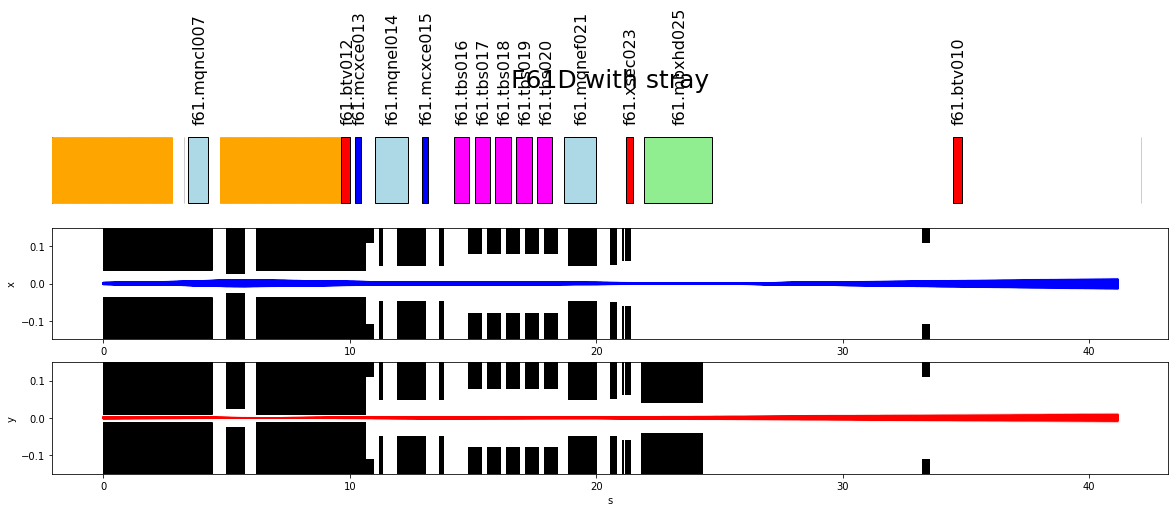
\includegraphics[width=1.0\textwidth]{02_Simulation/images/PTC_stray_field.png}
\caption{Stitched model PTC tracking.}
\label{fig:stitched_PTC}
\end{figure}

\subsection{Repository with the Full Stitching fomr the PS Ring to the East Dump}

The repository name is \href{https://gitlab.cern.ch/eljohnso/stray-fields}{stray-fields}. 

Step one, you need to create the distribution upstream of SEH23 using pycollimate. This is done in this \href{https://gitlab.cern.ch/eljohnso/stray-fields/-/blob/master/pycollimate.ipynb}{script} which gives you the distribution\_at\_seh23.pkl file.

Step two is to run \href{https://gitlab.cern.ch/eljohnso/stray-fields/-/blob/master/ps_ring.ipynb?ref_type=heads}{ps ring} which tracks the particle distribution in the PS ring and outputs the distribution before entering in the MU62

Step three is to run \href{https://gitlab.cern.ch/eljohnso/stray-fields/-/blob/master/f61d_tracking.ipynb?ref_type=heads}{f61d tracking} which takes the distribution entering in MU62 and tracking it in the F61D line.

\begin{figure}[H]
\centering
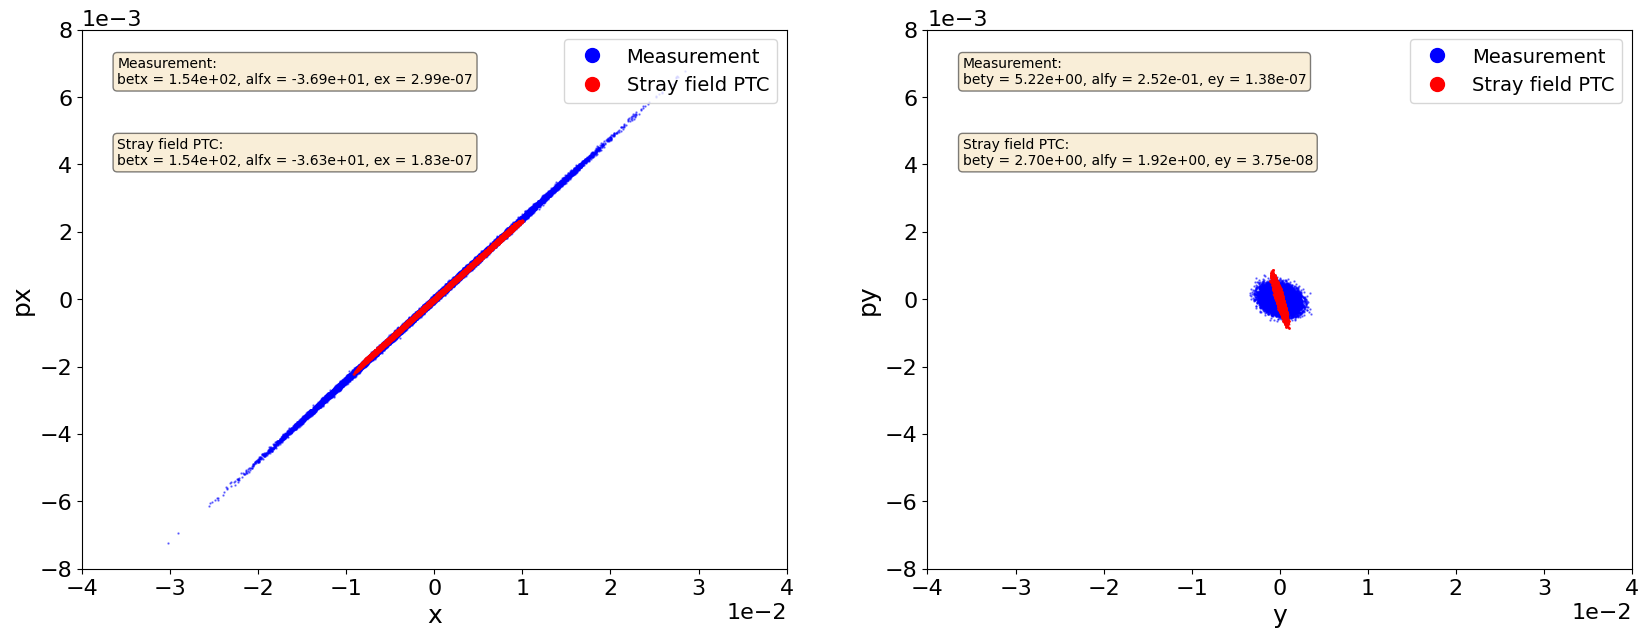
\includegraphics[width=1.0\textwidth]{02_Simulation/images/full_stitching_PTC.png}
\caption{Full Stitched model PTC tracking.}
\label{fig:full_stitched_PTC}
\end{figure}

Something to note is that the distribution from tracking is non gaussian so when computing the twiss parameters there might be some discrepancy.

\begin{figure}[H]
\centering
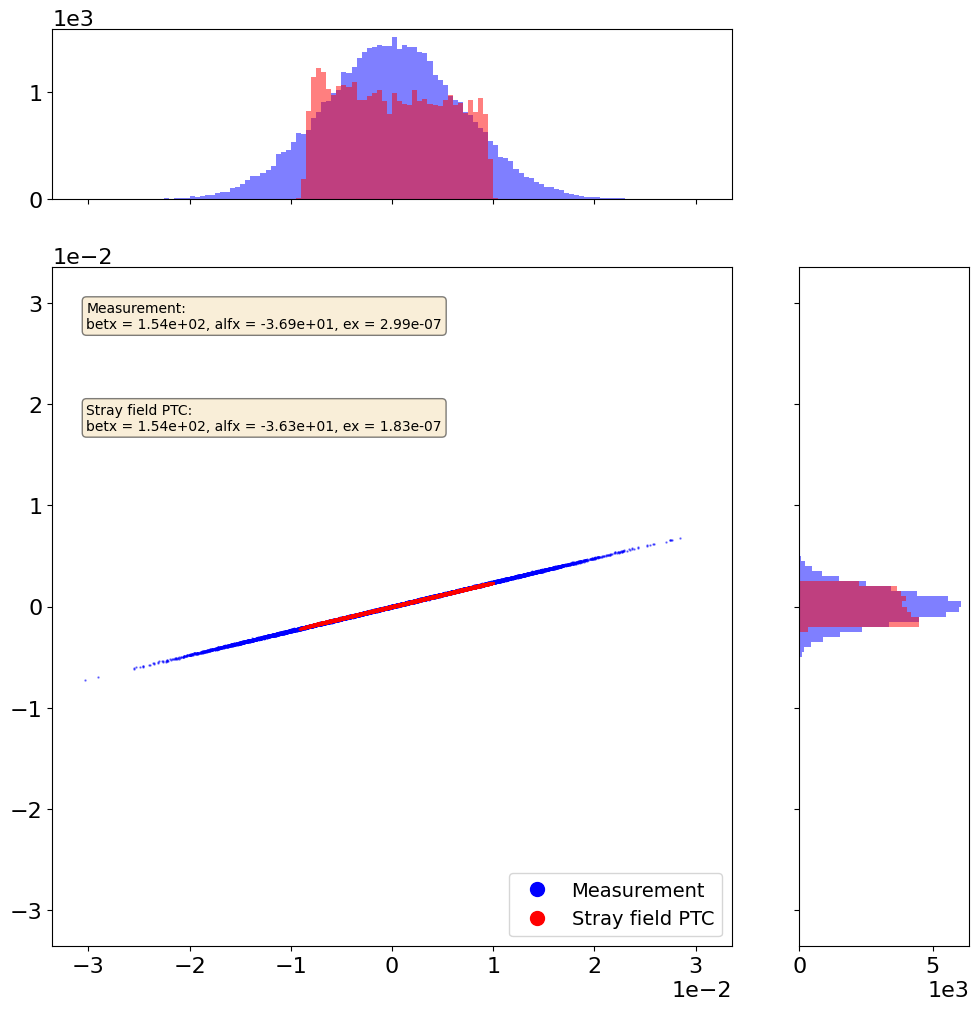
\includegraphics[width=1.0\textwidth]{02_Simulation/images/non_gaussian.png}
\caption{The distributions are not gaussian.}
\label{fig:full_stitched_PTC}
\end{figure}

Perhaps instead of showing distribution of particles it is interesting to see the difference in the ellipses, see Fig. \ref{fig:ellipses.}.

\begin{figure}[H]
\centering
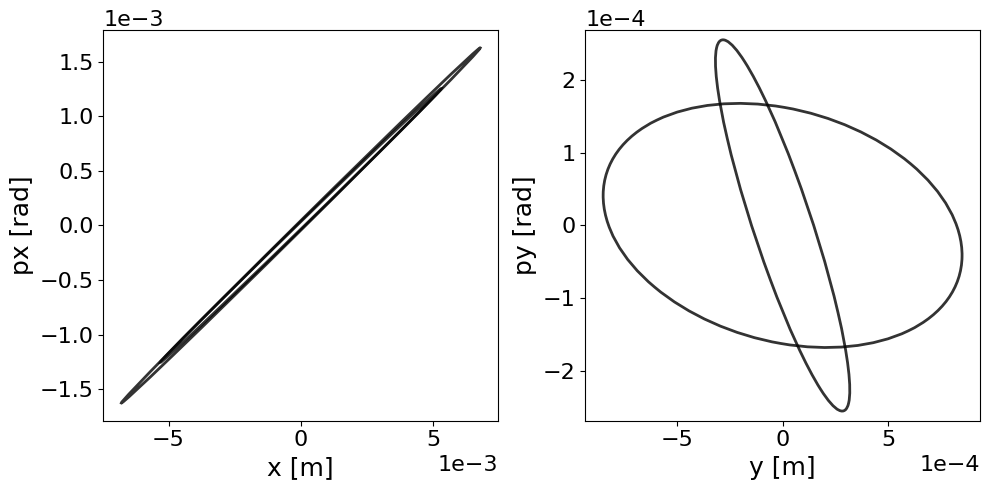
\includegraphics[width=1.0\textwidth]{02_Simulation/images/ellipses.png}
\caption{Comparison between the ellipses produces by the twiss parameters of the simulation and the tracking.}
\label{fig:ellipses.}
\end{figure}

We can also have a look at the twiss parameters evolution along the line, see Fig. \ref{fig:twiss_params}.

\begin{figure}[H]
\centering
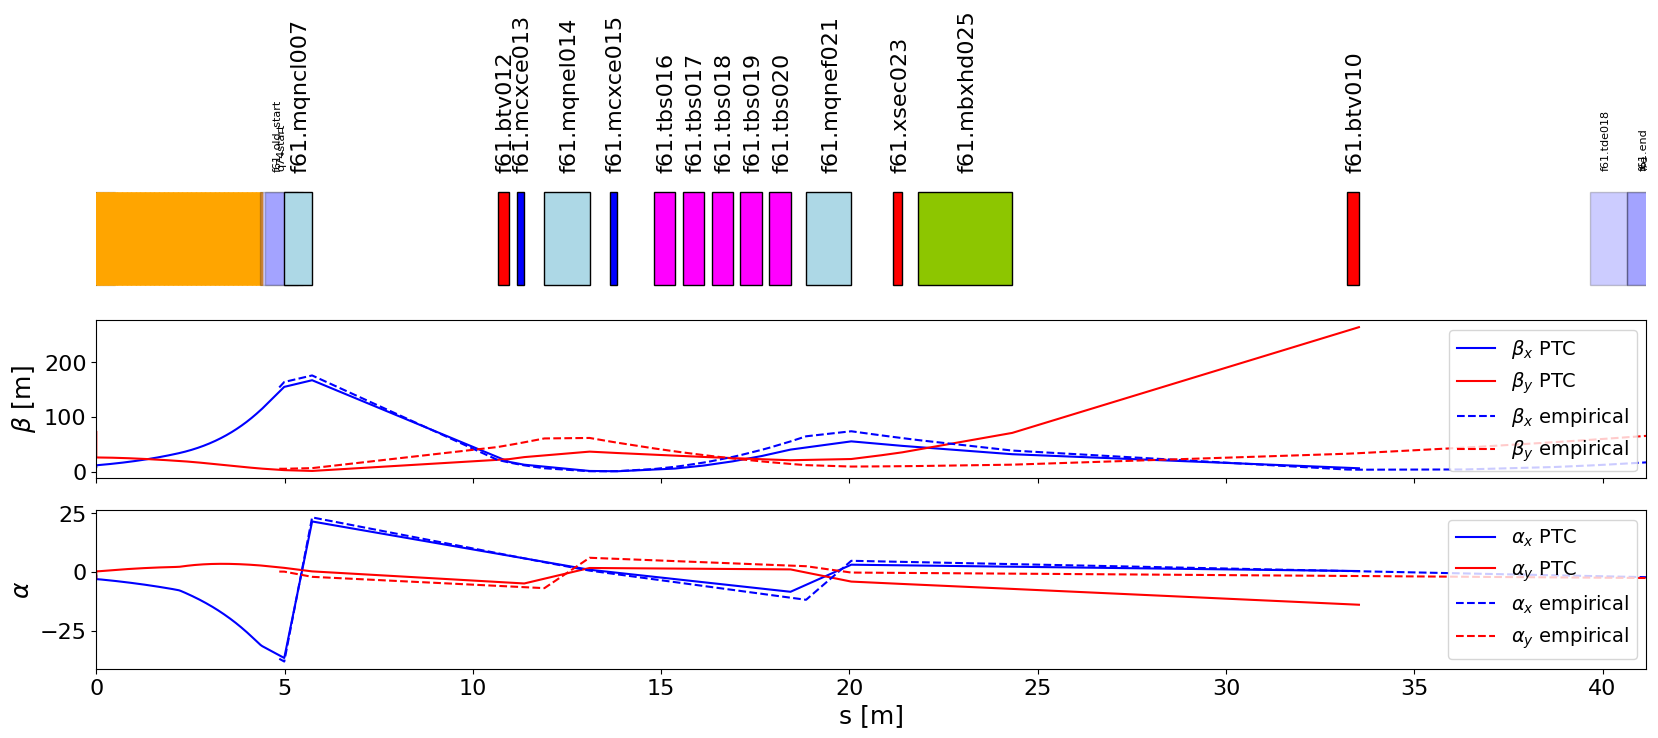
\includegraphics[width=1.0\textwidth]{02_Simulation/images/twiss_parameters_comparison.png}
\caption{Comparison between the twiss parameters along the line of the simulation and the tracking.}
\label{fig:twiss_params}
\end{figure}

\subsection{Simulation of Transfer Matrix Using Tracking at Injection}

The following subsection describes the methodology and findings from a simulation study aimed at constructing a transfer matrix for the injection process in the Proton Synchrotron (PS) using tracking techniques. The primary objective is to evaluate the response of injected particles to various initial offsets and to compare the results with existing models.

A comprehensive simulation was performed using the  \href{https://gitlab.cern.ch/eljohnso/acc-models-tls-eliott-fork/-/blob/EliottBranch/ps_injection/kick_response_injection_tracking/kick_response_BTP_injection_loop_transfer_matrix.ipynb}{kick response BTP injection loop transfer matrix} notebook. This notebook tracks particles injected into the PS at different initial offsets in the transverse and longitudinal planes. Specifically, four types of initial offsets were used: horizontal position (\(x_{in}\)), horizontal angle (\(p_{x,in}\)), vertical position (\(y_{in}\)), and vertical angle (\(p_{y,in}\)). The resulting offsets at the output (\(x_{out}\), \(p_{x,out}\), \(y_{out}\), \(p_{y,out}\)) were recorded to construct the transfer matrix.

\begin{figure}[H]
\centering
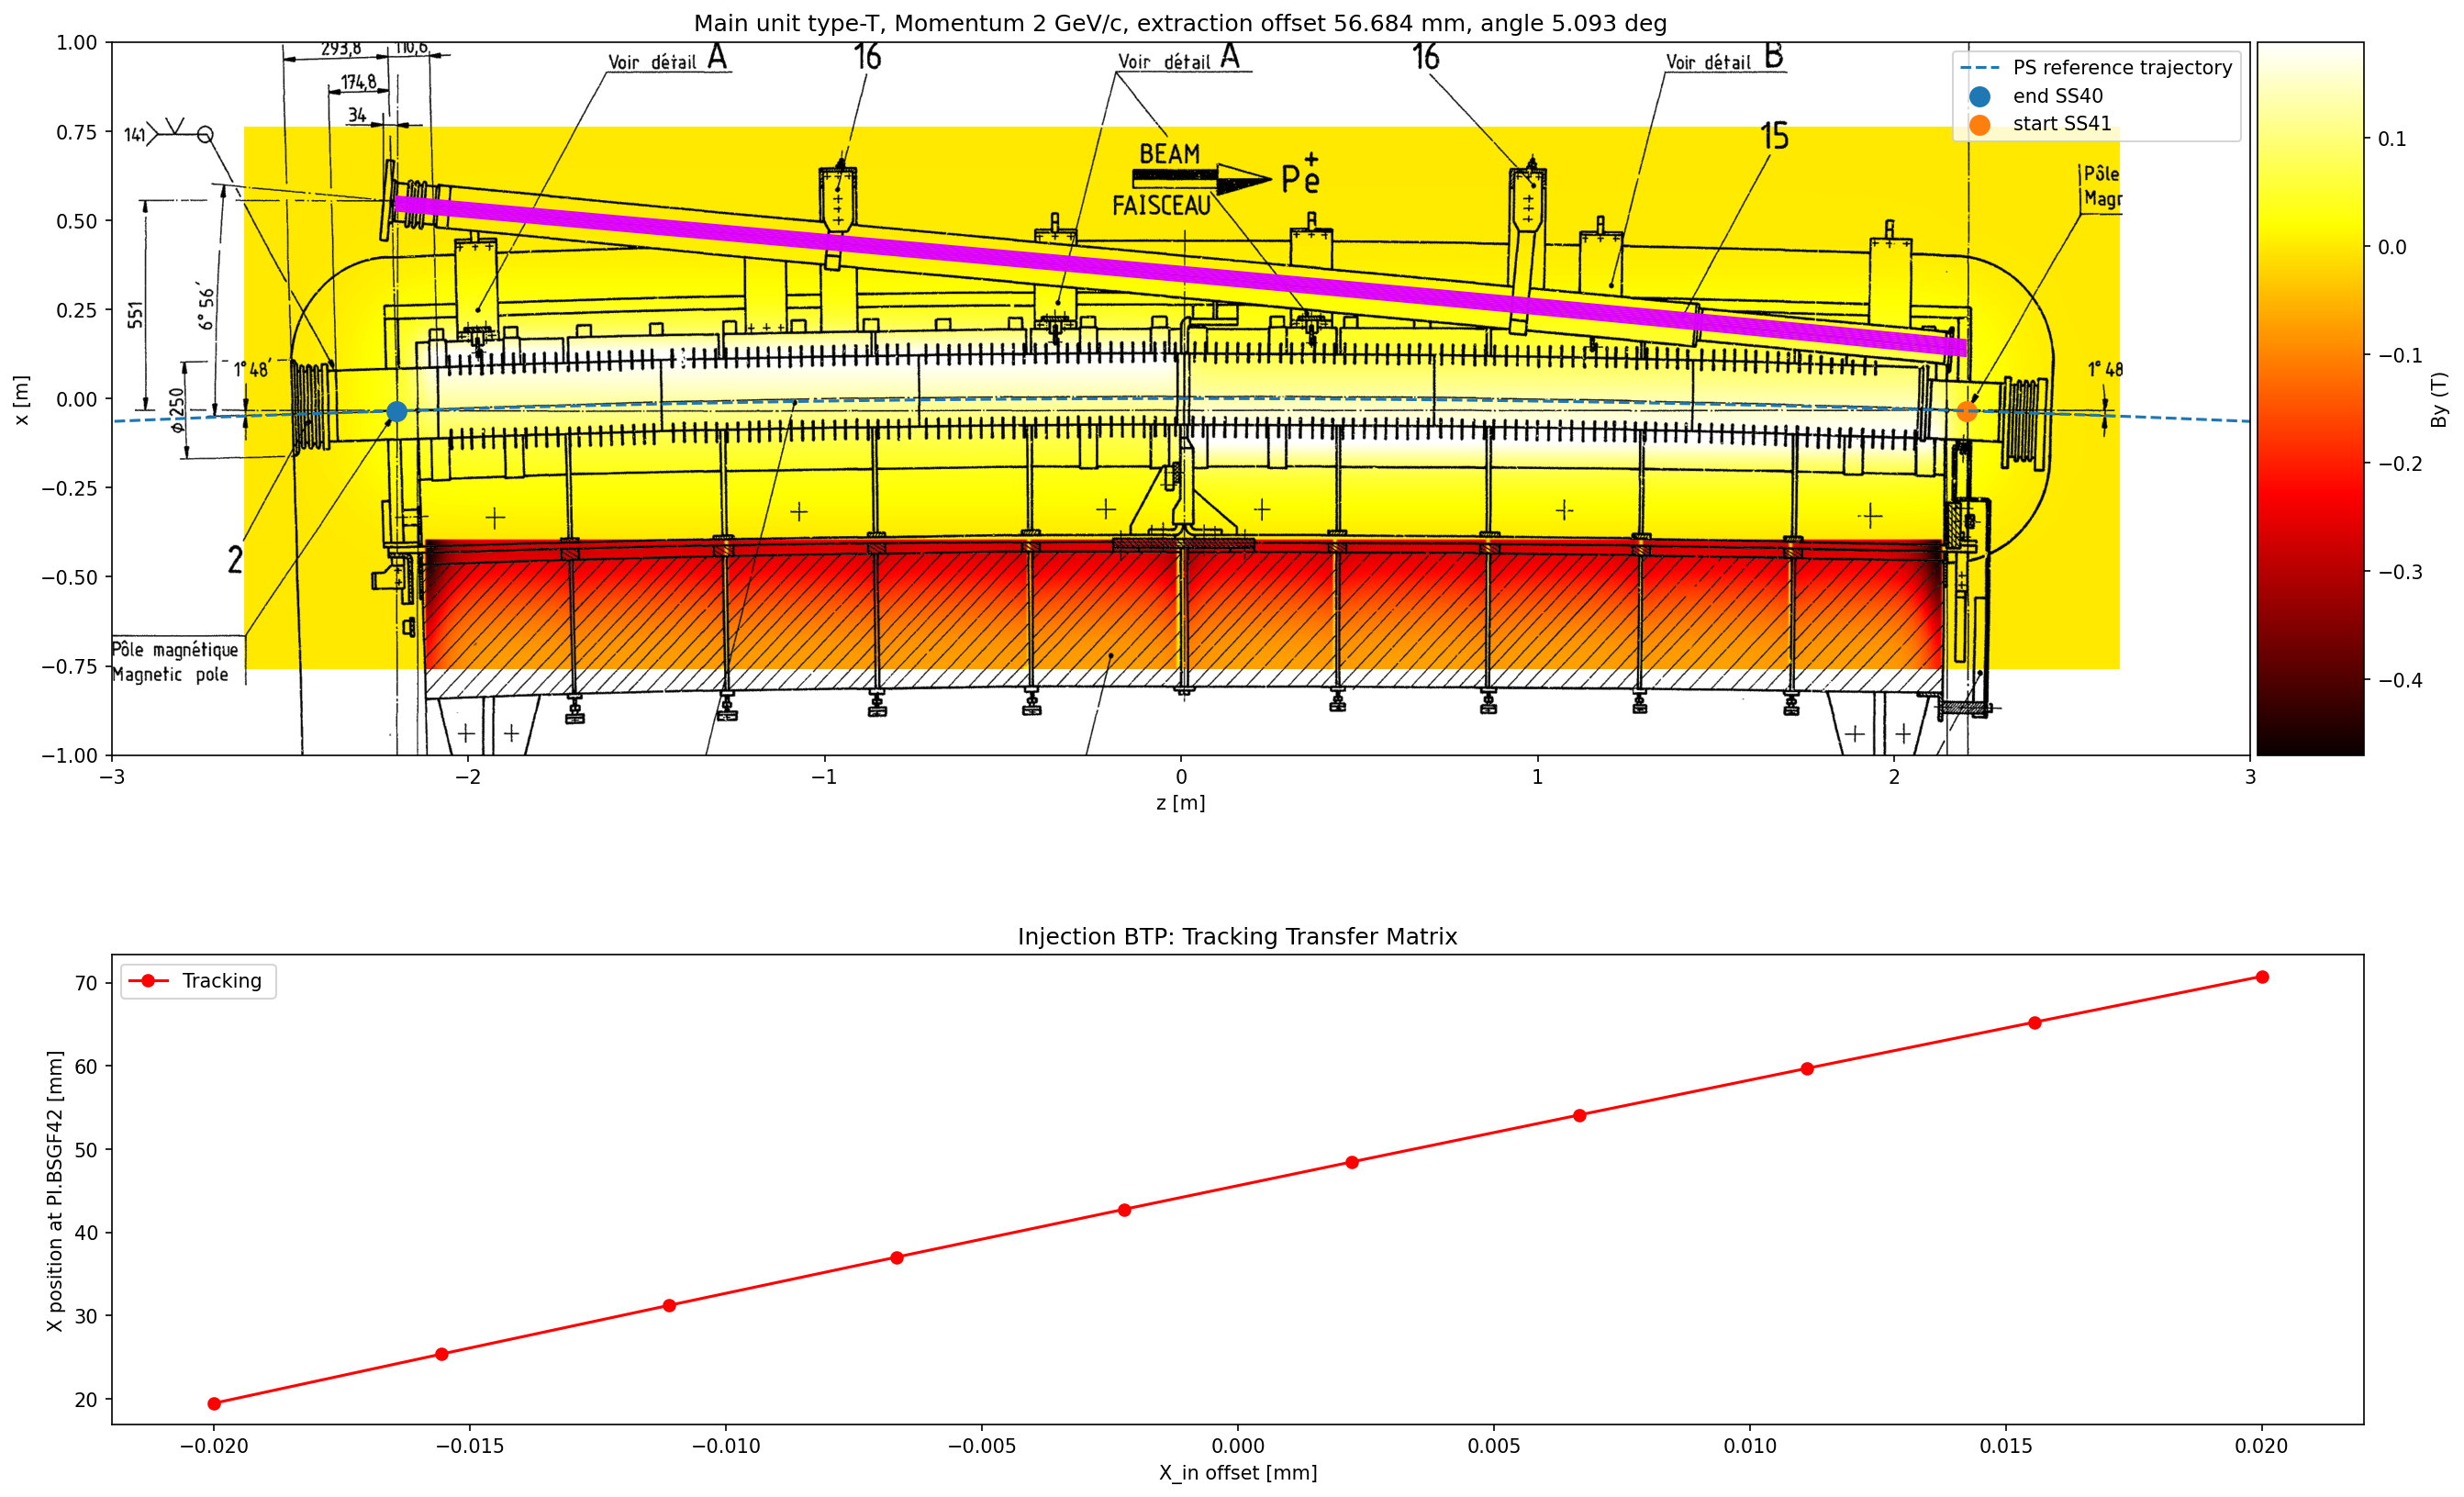
\includegraphics[width=1.0\textwidth]{02_Simulation/images/injection_transfer_matrix_1.png}
\caption{Building a transfer matrix through tracking.}
\label{fig:transfer_matrix_1}
\end{figure}

\begin{figure}[H]
\centering
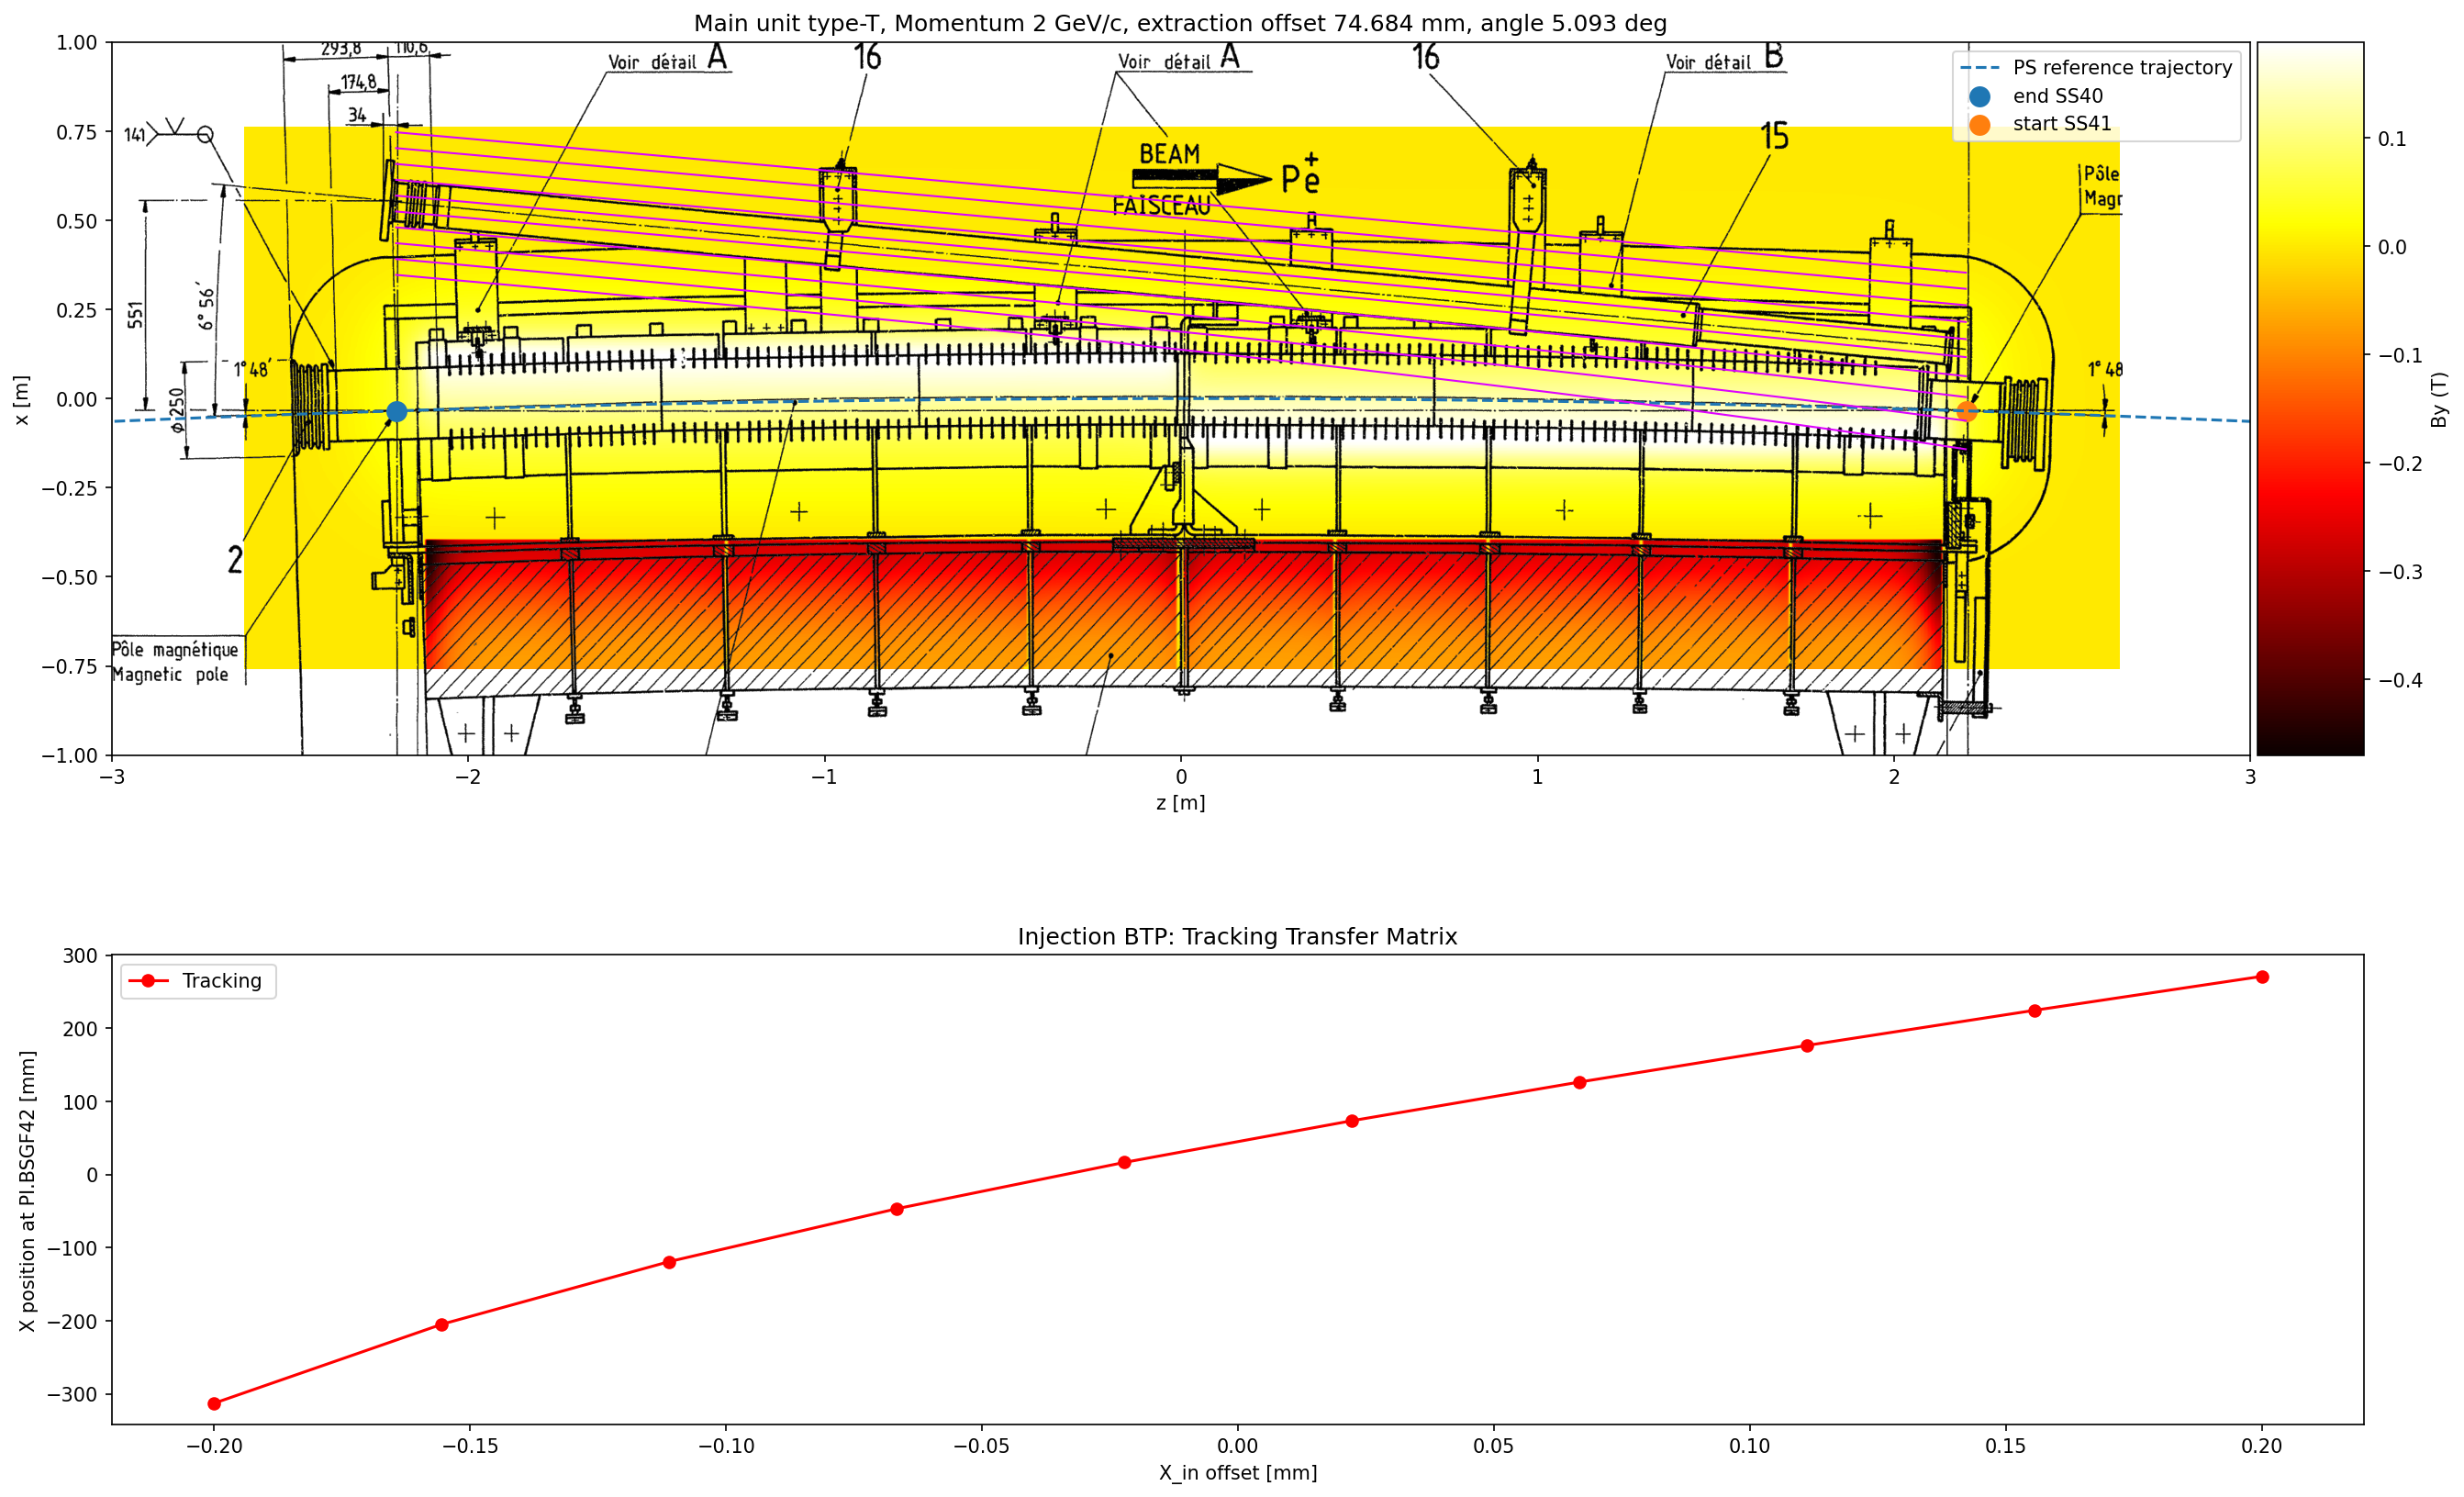
\includegraphics[width=1.0\textwidth]{02_Simulation/images/injection_transfer_matrix_2.png}
\caption{Wide scan of the position offset to see if the response is non-linear.}
\label{fig:transfer_matrix_2}
\end{figure}


The simulation can cover a wide range of offsets to capture potential non-linearities. The wide scan shown in Fig. \ref{fig:transfer_matrix_2} launches particles at transverse offsets that extend beyond the vacuum chamber, showing the non-linear beam dynamics.

As such, the technique to build a transfer matrix is to launch particles with four kind of input offsets: $x_{in}$, $xp_{in}$, $y_{in}$, $yp_{in}$ and record the output offsets $x_{out}$, $xp_{out}$, $y_{out}$, $yp_{out}$.

\begin{figure}[H]
\centering
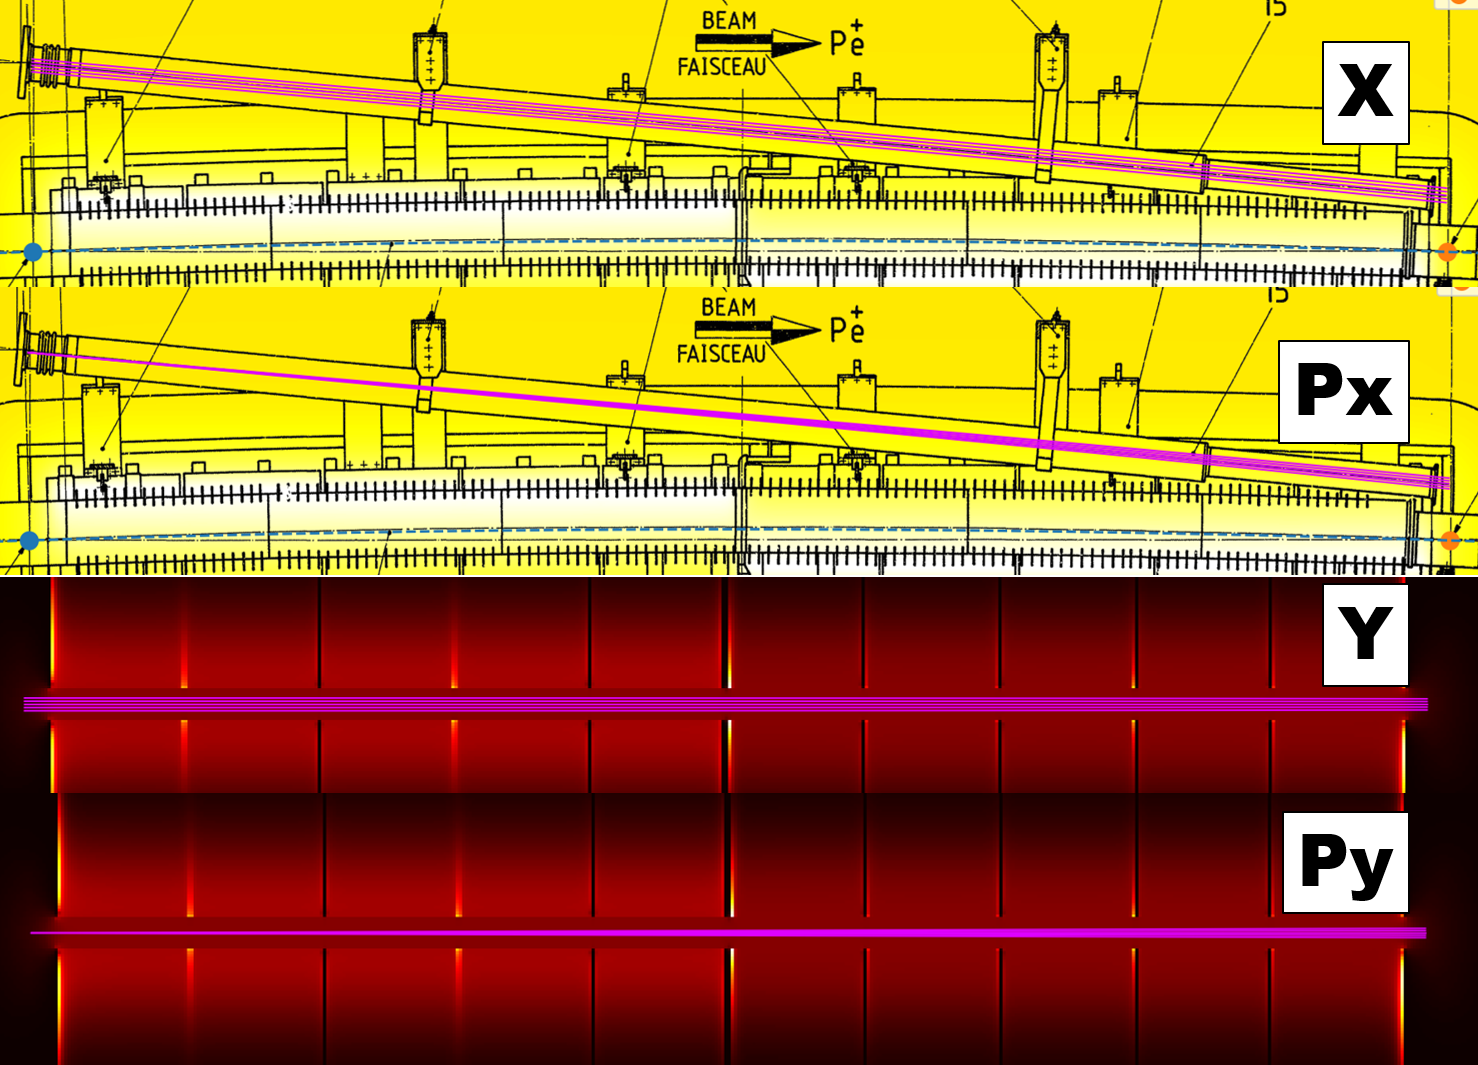
\includegraphics[width=1.0\textwidth]{02_Simulation/images/injection_transfer_matrix_3.png}
\caption{Particles are launched with different offsets.}
\label{fig:transfer_matrix_3}
\end{figure}

Figure \ref{fig:transfer_matrix_4} shows the transfer matrix points between the start and the end of the tracking inside the main unit. A linear fit is used to calculate the slope.

\begin{figure}[H]
\centering
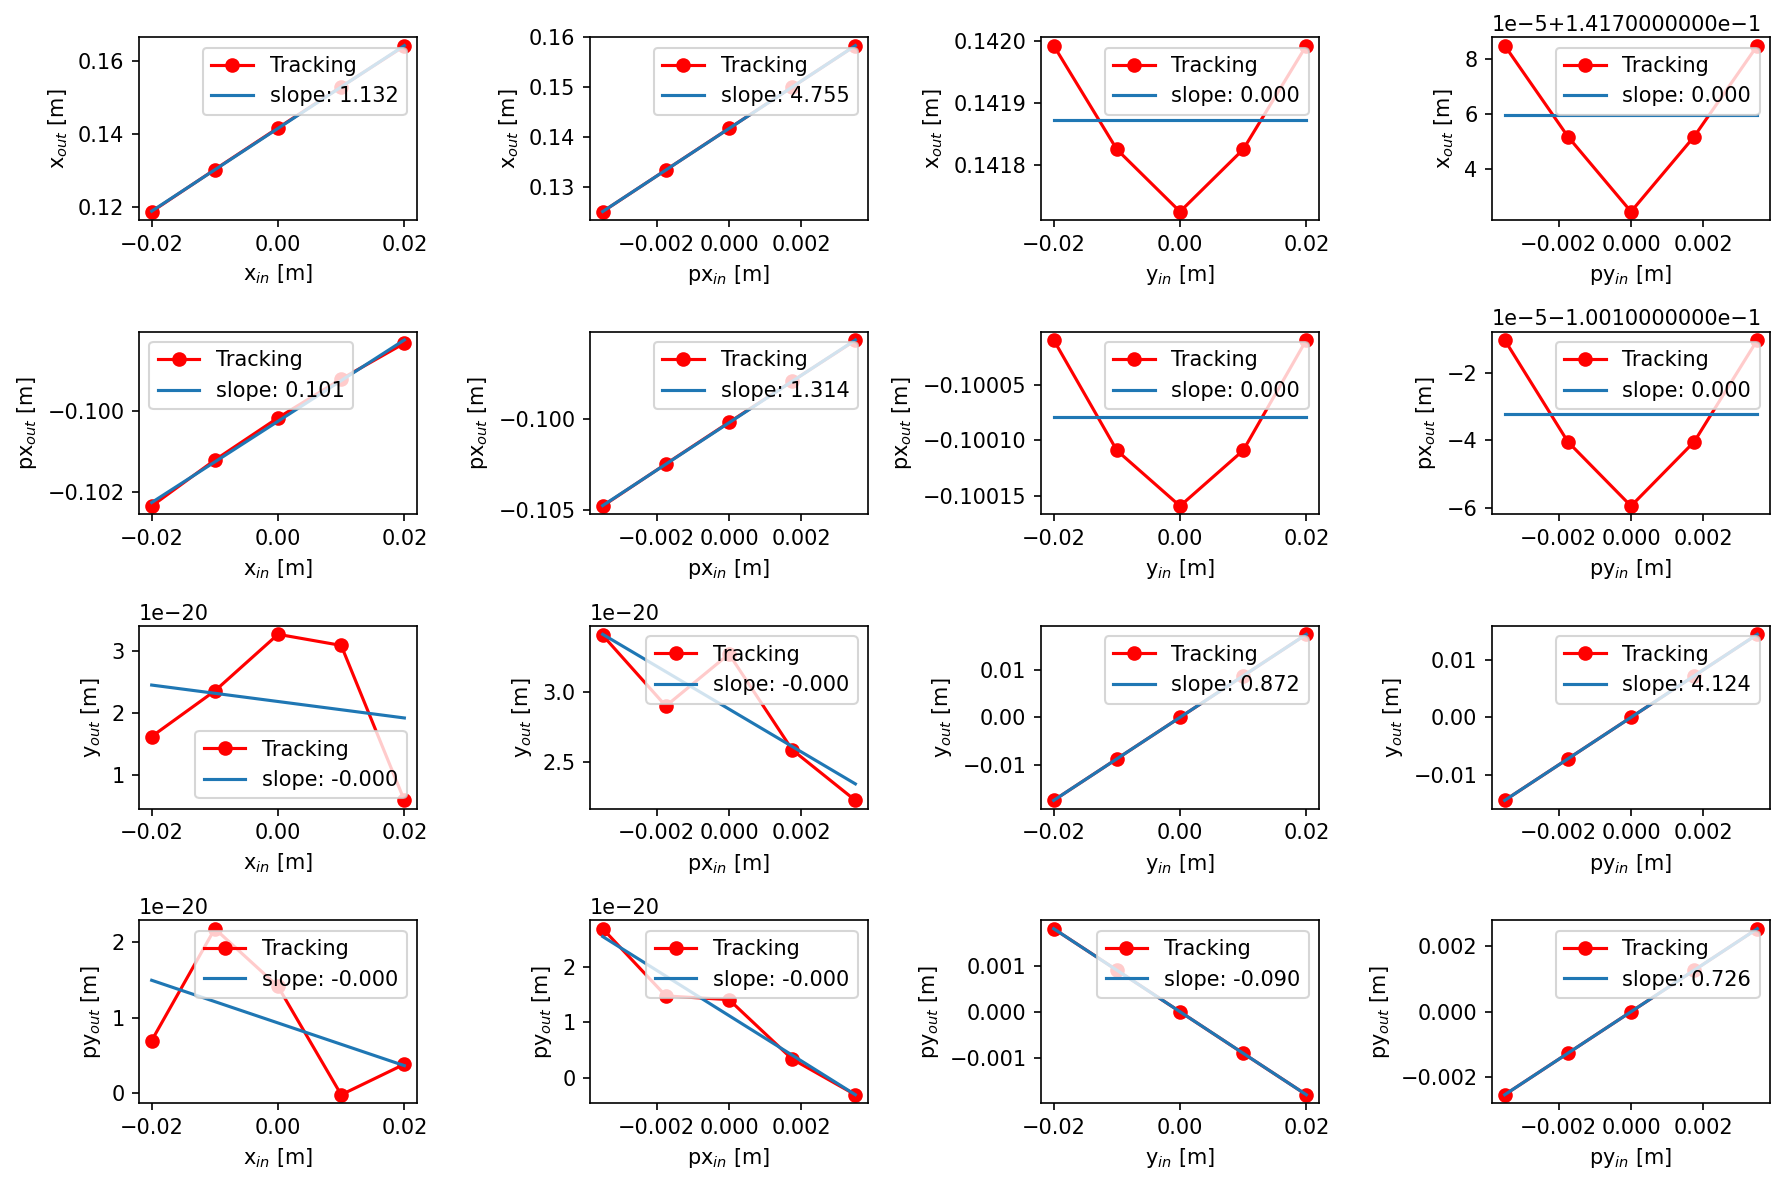
\includegraphics[width=1.0\textwidth]{02_Simulation/images/injection_transfer_matrix_4.png}
\caption{Particles are launched with different offsets.}
\label{fig:transfer_matrix_4}
\end{figure}



\textbf{Matrix from Tracking:}
\[
\begin{bmatrix}
1.132 & 4.755 & 0 & 0 \\
0.101 & 1.314 & 0 & 0 \\
0 & 0 & 0.872 & 4.124 \\
0 & 0 & -0.090 & 0.726
\end{bmatrix}
\]

The transfer matrix can also be visualized using color maps and compared to another transfer matrix tool developed by Ewa (called tracks.get\_transport\_matrix(k = k\_last, ret = 'mat')). Ewa's method eliminates the need for computationally intensive tracking. Instead, the nominal tracking can be used in conjunction with Ewa's function. However, it is important to note that this approach is only valid for the tracking section and does not extend to the SEM-Grid.

\begin{figure}[H]
\centering
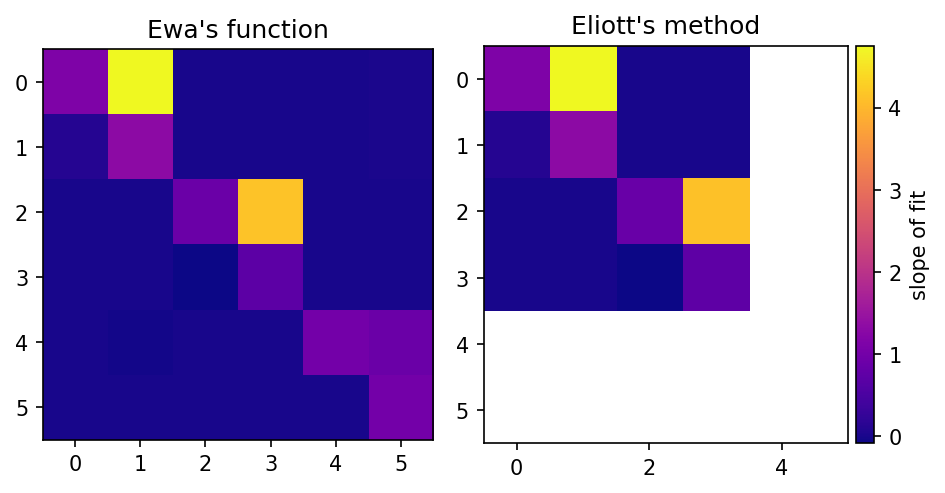
\includegraphics[width=1.0\textwidth]{02_Simulation/images/transfer_matrix_color.png}
\caption{Comparison between the matrix found by tracking at different offsets and Ewa's function.}
\label{fig:transfer_matrix_color}
\end{figure}





A transfer matrix, see Fig. \ref{fig:transfer_matrix_color}, can also be built as a function of POPS (from \si{500} to \si{1500}{gauss}) where it is observed that the injection angles are very sensitive to POPS change. The transfer matrix shows that injection angles are twice the sensitivity compared to horizontal (\(x\)) or vertical (\(y\)) offsets. This implies that any increase in POPS will significantly amplify the effect of a change in the horizontal angle (\(p_x\)) on the horizontal offset (\(x\)). Specifically, the matrix elements \(R_{21}\) and \(R_{22}\) exhibit the most substantial positive changes, indicating a strong correlation between \(p_{x,\text{in}}\) and both \(x_{\text{out}}\) and \(p_{x,\text{out}}\). Conversely, \(R_{34}\) and \(R_{44}\) show the most significant negative changes, highlighting the impact of \(p_{y,\text{in}}\) on both \(y_{\text{out}}\) and \(p_{y,\text{out}}\). These findings underscore the critical influence of POPS variations on beam dynamics, particularly in relation to injection angles.

\begin{figure}[H]
\centering
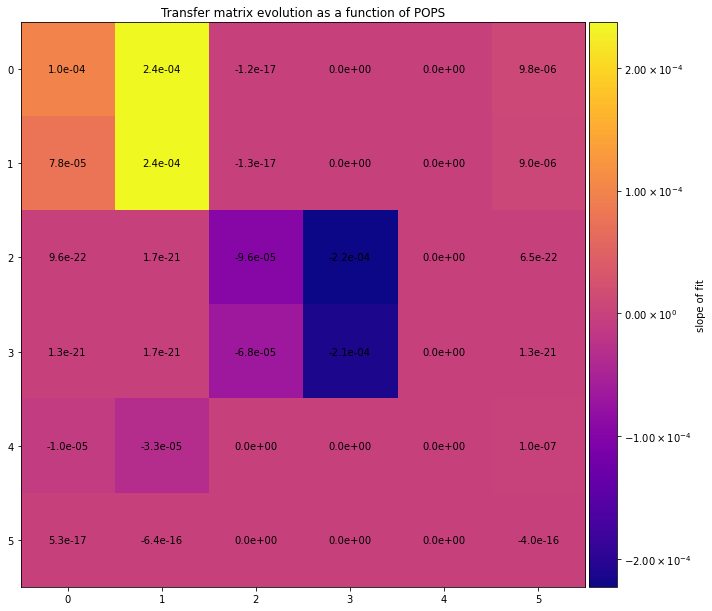
\includegraphics[width=1.0\textwidth]{02_Simulation/images/transfer_matrix_POPS.png}
\caption{Transfer matrix evolution as a function of POPS}
\label{fig:transfer_matrix_pops}
\end{figure}

The established transfer matrices can be utilized in MAD-X simulations to predict beam sizes under varying conditions. Notably, the elements \(R_{21}\), \(R_{22}\) (corresponding to \(p_{x,in}/x_{out}\) and \(p_{x,in}/p_{x,out}\)), and \(R_{34}\), \(R_{44}\) (corresponding to \(p_{y,in}/y_{out}\) and \(p_{y,in}/p_{y,out}\)) exhibited the most significant changes with variations in POPS, underscoring their critical role in beam dynamics at injection.


The source code for the simulations can be found in the following repositories:
\begin{itemize}
  \item \href{https://gitlab.cern.ch/eljohnso/acc-models-tls-eliott-fork/-/blob/EliottBranch/ps_injection/kick_response_injection_tracking/kick_response_BTP_injection_loop_transfer_matrix.ipynb}{Notebook: kick response BTP injection loop transfer matrix}
  \item \href{https://gitlab.cern.ch/eljohnso/acc-models-tls-eliott-fork/-/blob/EliottBranch/ps_injection/kick_response_injection_tracking/kick_response_BTP_injection_loop_transfer_matrix_function_of_POPS.ipynb}{Notebook: kick response BTP injection loop transfer matrix function of POPS.ipynb}
\end{itemize}


\subsection{Talk about how the shims are not implemented in OPERA and the solution in MAD-X}

\subsection{New chapter on extraction in F16}

%%%%%%%%%%%%%%%%%%%%%%%%%%%%%%%%
%%%% Empirical Measurements %%%%
%%%%%%%%%%%%%%%%%%%%%%%%%%%%%%%%

\section{Empirical Measurements}
\label{section:Empirical_measurements}

% Begin this section with a brief introduction about what empirical measurements are, why they are necessary, and what they aim to determine or reveal in the context of stray fields in the PS

\subsubsection{Measurement of the extracted beam parameters}

Quadrupole scans have been performed to reconstruct the beam parameters in the East Area extraction line. The beam size was measured with Beam instrumentation - TV (BTV) screens as the strength of one or multiple quadrupoles was varied. The initial parameters can be determined empirically by fitting them to a MAD-X simulation against the measurements. BTVs are not ideal instruments for performing these measurements; they saturate at the extraction intensities, and the signal must be fitted with care. Filter wheels have been installed to reduce saturation, allowing for more accurate initial parameter measurement. In addition, a dispersion measurement will be performed to reduce the degrees of freedom of fit.
Kick response measurements have also been carried out. Future studies will compare the initial parameters measured with those predicted by tracking through the field maps in MAD-X.


Empirical measurements provide a fundamental foundation for validating and improving simulation models, particularly in examining the initial conditions of the beam at the PS exit. These assessments are conducted through quadrupole scans at the East Dump.

\begin{figure}[htbp]
\centering
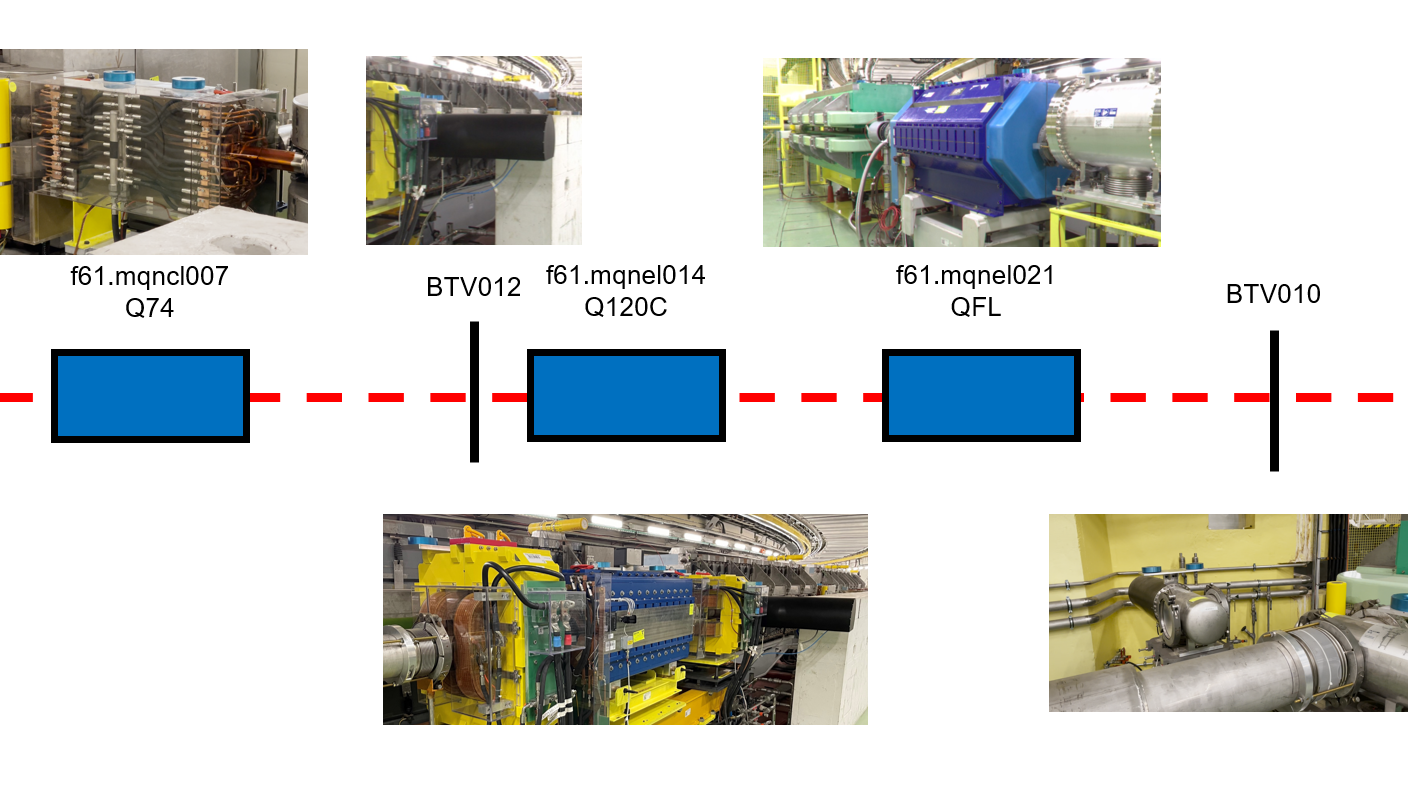
\includegraphics[width=\linewidth]{03_Empirical_Measurements/images/East_dump_line.png}
\caption{Diagram of the East Dump Line which comprises three quadrupoles and a bending magnet that directs the beam to the dump (F6D.TDE018). Two BTVs (BTV012 and BTV010) are used for beam measurements.}
\label{fig:East_dump_line}
\end{figure}

Situated within the East Area complex is a short line, designed for extraction studies, which leads to a dump aptly named the East Dump Line, see Fig. \ref{fig:East_dump_line}. The East Dump Line is ideally suited for quadrupole scans due to its configuration of three upstream quadrupoles used to modify the optics. Additionally, it houses two Beam-TV (BTVs) (F61.BTV012 and F61D.BTV010) for beam observation. Notably, the line can be used for parallel Machine Development (MD) without disrupting operational beams directed at the experimental targets in the East Area. Each BTV employs a fluorescent screen which can be remotely inserted into the beam line during measurements, see Fig. \ref{fig:btv_diagram}. The interaction of the particles with the material produces light which a camera system subsequently captures through a viewport. The image collected corresponds to the beam "footprint" on the screen, serving a valuable tool for beam observation, steering or measurement. The insertion of the screen has the downside of significantly degrading the beams properties, such as the beam size, through material interaction and care must be taken when used in parallel of other beams. This issue doesn't not concern the East Dump line as BTV010 is placed in front of the East Dump which can be used exclusively for extraction and optics MDs.

\begin{figure}[htbp]
\centering
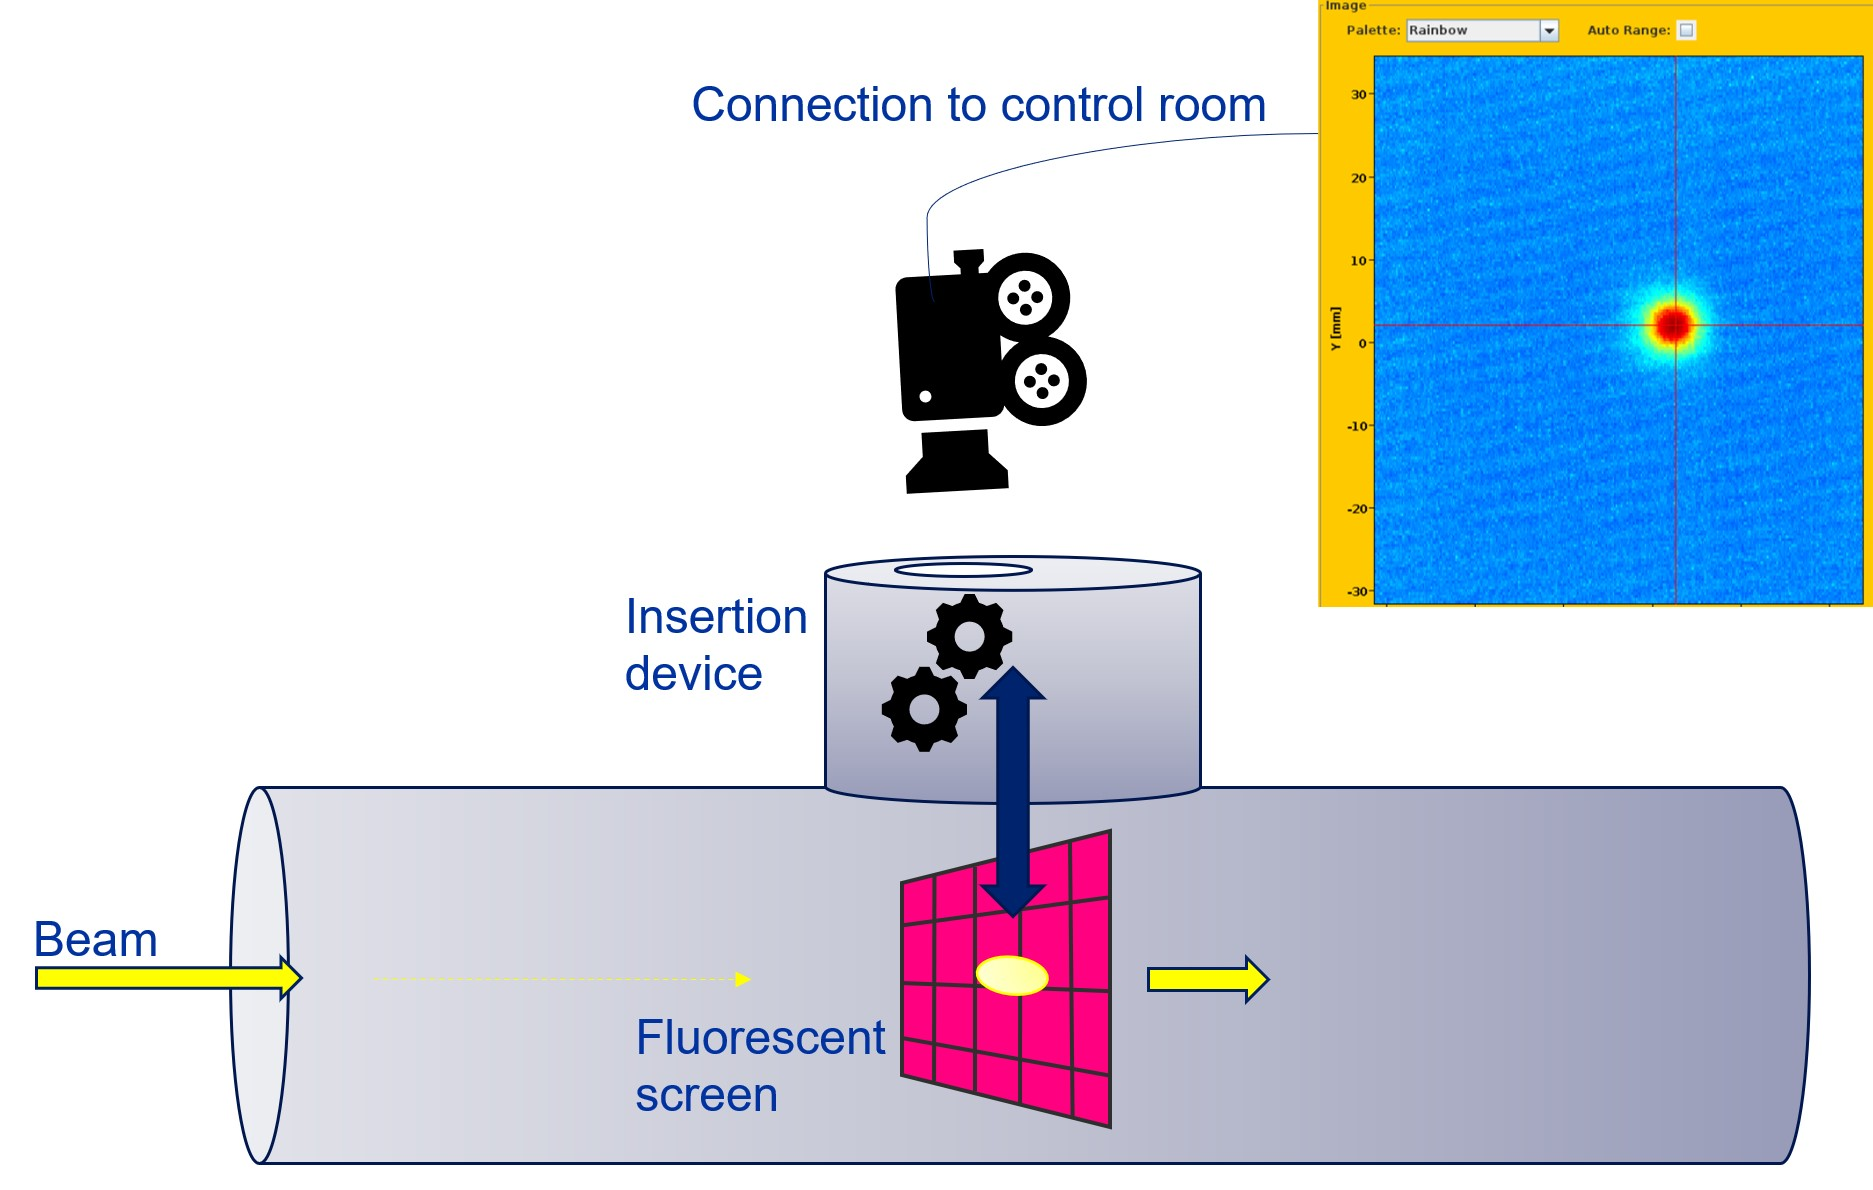
\includegraphics[width=0.7\linewidth]{03_Empirical_Measurements/images/BTV_diagram.jpg}
\caption{BTV Diagram}
\label{fig:btv_diagram}
\end{figure}

\subsection{Quadrupole scan}
\label{Quadrupole Scan}

% Describe the process and the purpose of the quadrupole scan. You should discuss:
% The objective of the scan.
% The setup: What equipment is used? How is the experiment arranged?
% The process: How is the scan conducted?
% The results: What data was collected? What are the key findings from the scan?

A quadrupole scan is used to measure beam parameters and involves adjusting the strength of a quadrupole, and subsequently observing the variations in the beam size ($\sigma$) and beam position (centroid) across both planes using an instrument located downstream of the quadrupole being modified, see Fig. \ref{fig:quad_scan_example}. The objective of this scan is to finely tune the simulation tool MAD-X \cite{noauthor_mad_nodate} to enable the prediction of beam sizes through a model that has been adjusted according to these measurements. To achieve this, the initial parameters of the MAD-X model are aligned with the observed measurements as accurately as possible. It is generally advantageous to find the minimum and maximum values of the beam size at the instrument's location, which facilitates the reconstruction of the rematching of the initial conditions. The parameter-matching process is conducted in Python, utilizing either the Scipy or the Py-BOBYQA library \cite{cartis_improving_2019, cartis_escaping_2022}.

\begin{figure}[htbp]
\centering
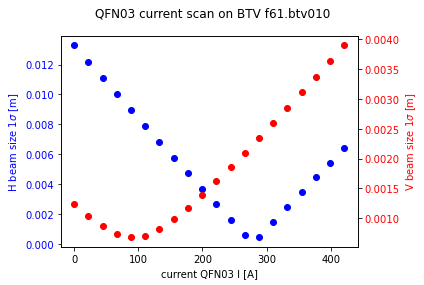
\includegraphics[width=0.5\linewidth]{03_Empirical_Measurements/images/quadrupole_scan_east_dump.png}
\caption{Example of a quadrupole scan with minimums in both planes measured on the East Dump BTV.}
\label{fig:quad_scan_example}
\end{figure}

A quadrupole scan can also serve as a tool to inform about the relative offset between the beam and the quadrupole's center. Operationally, there is a high likelihood that the beam is not perfectly centered within a quadrupole. In such instances, any alteration in the quadrupole's strength will not only affect the beam size or the optics, which is the expected primary effect, but will also induce a dipole moment. This, in turn, will shift the centroid of the beam. In simpler terms, if a scan in current/strength of a quadrupole is conducted, and there is a misalignment in either the beam or the quadrupole, it will result in the beam being steered. Figure \ref{fig:misaligned_quadrupole} provides a simulation of the East Dump Line with the first quadrupole misaligned by a positive offset of 0.01 m in the x direction (to the left in the beam's path). The color-coded traces illustrate the different paths that the particle will follow as the quadrupole's strength is adjusted. This however cannot distinguish between the quadrupole being offset and the beam being mis-steered.
\\

\begin{figure}[htbp]
\centering
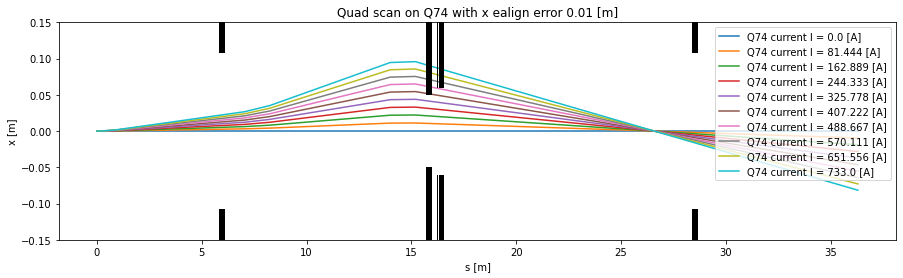
\includegraphics[width=\linewidth]{03_Empirical_Measurements/images/misaligned_quadrupole.png}
\caption{MAD-X simulation of a quadrupole being misplaced and impact of quadrupole strength variation.}
\label{fig:misaligned_quadrupole}
\end{figure}

Figure \ref{fig:misaligned_quadrupole_2} displays the displacement of the centroid as a function of current, with the quadrupole Q74 being misaligned by different values. This plot can help understand in which direction the beam will move and by how much if not properly centered. Additionally and important to note an offset in the beam position will not modify the beam size.
\\

\begin{figure}[htbp]
\centering
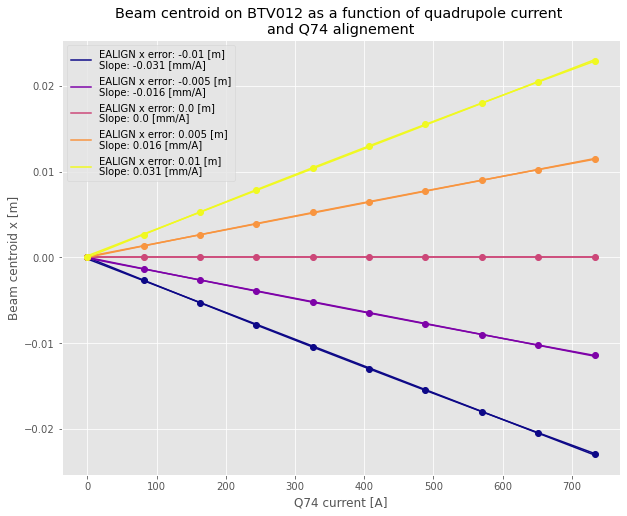
\includegraphics[width=0.7\linewidth]{03_Empirical_Measurements/images/misaligned_quadrupole_2.png}
\caption{Misaligned quadrupole simulation}
\label{fig:misaligned_quadrupole_2}
\end{figure}

CERN frameworks facilitate the adjustment of current in specific quadrupoles through Python, utilizing a library known as PyJapc \cite{noauthor_scripting-tools_2023}. A suite of quadrupole scan scripts, employed in this note, can be accessed via the following GitLab repository:  \href{https://gitlab.cern.ch/eljohnso/quad-scan-east}{gitlab.cern.ch/eljohnso/quad-scan-east}. Referring to the quadrupole beam offset just discussed, a simple script called \href{https://gitlab.cern.ch/eljohnso/quad-scan-east/-/blob/master/check_centered_in_quad.py}{check\_centered\_in\_quad.py} scans three currents in a specific quadrupole and looks at the mean position of the gaussian fit on a BTV. It continuously takes the last three centroid measurement ($\mu$) which can be used for informed beam steering.

\subsubsection{East Area BTV}
BTVs are one of the instrumentation used in this report and some explanation on how they operate is required. Specific to the extraction in the East Area is that during a slow extraction ($\sim$ \SI{400}{ms}) the BTVs are capable of multiple acquisitions. This can be used to take the multiple beam size measurements during the spill and observe any difference in beam position or trend such as a sweep. As it turns out, the beam size changes during the spill which means the optics during extraction isn't constant. This is why when finding initial parameters or rematching a single acquisition from the BTV was chosen (in the middle of the spill) to best represent the beam. Most of the time the fourth acquisition was chosen as it is once the beam is stabilised (after the Figure-of-eight Loop's (F8L) eddy currents). The East Area BTV system is comprised of two crates: cfv-157-btv1, which includes PR57, F62, F61, and F61D, and cfv-157-btv2, which includes all T8 BTVs. There are three crucial parameters that can be changed in these two crates: PE2X.SACQ-EMTV2 (\textbf{S}tart \textbf{ACQ}uisition), PE2X.ACQ-EMTV2 (delay between \textbf{ACQ}uisition), and PE2X.EACQ-EMTV2 (\textbf{E}nd \textbf{ACQ}uisition).

\begin{enumerate}
    \item The PE2X.SACQ-EMTV2 parameter is adjustable, with a caveat that the initial event is lost due to the offset of the initiation timing. Presently, the acquisition begins 900 ms prior 1030 ms extraction start, plus an additional 720 ms delay, culminating in a start time at 850 ms. The first acquisition occurs at 950 ms (850 plus a 100 ms delay) with subsequent acquisitions every 100 ms, see Fig. \ref{fig:btv_timing}. Previously, the start timing for the BTVs began at PE2X-W20, a 20 ms pre-extraction warning. However, BI made modifications such that the timing now starts at PE2X.F900-CT, a 900 ms forewarning before extraction. The starting event can be verified through LTIM cfv-157-btv2.LTIM and PE2X.SACQ-EMTV2/LoadEvent.
    \item The PE2X.ACQ-EMTV2 parameter determines the interval between each image acquisition. By setting this parameter to zero and scrutinizing the acqTimeInCycle, it is possible to compute the time required for each acquisition which is $\sim$ 70 ms.
    \item The PE2X.EACQ-EMTV2 parameter signals the end of the acquisition period, which begins at PX.ELFT-CT, marking the \textbf{E}nd of the flat top (\textbf{FT}) cycle plus an additional 200 ms. This parameter is configured in such a way as to ensure that the seven acquisition instances occur within each cycle (lasting 2400 ms).
\end{enumerate}

\begin{figure}[H]
\centering
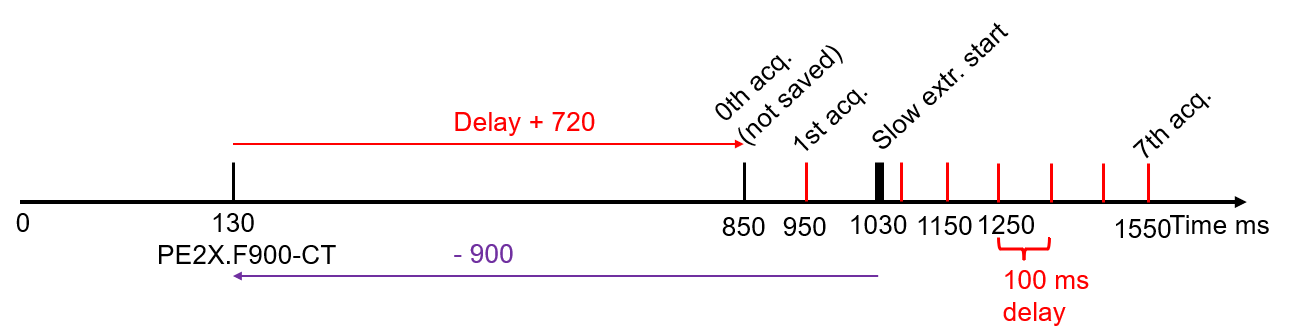
\includegraphics[width=1.0\linewidth]{03_Empirical_Measurements/images/btv_timing.png}
\caption{East Area BTV timing}
\label{fig:btv_timing}
\end{figure}


The BTVs operate asynchronously, leading to a jitter of 20 ms between each frame, see Fig. \ref{fig:btv_jitter}. However, with the imposed delay, we plan for an empty frame at the beginning, which can be used for background noise removal. It is possible to install a hardware trigger to remove the jitter as it is done in the other lines but this is currently not installed in the East Area.

\begin{figure}[ht]
\centering
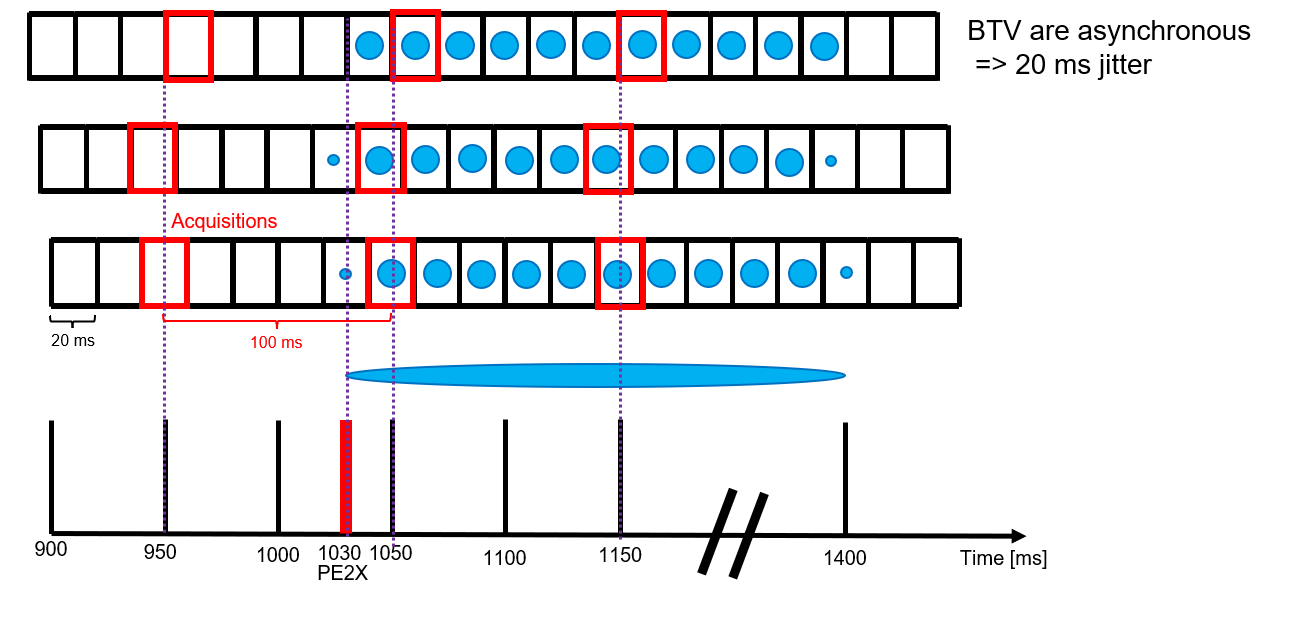
\includegraphics[width=1.0\linewidth]{03_Empirical_Measurements/images/btv_jitter.png}
\caption{BTV jitter}
\label{fig:btv_jitter}
\end{figure}

The fastest achievable full-resolution acquisition occurs with a delay of 90 ms. Further reduction of the delay yields inconsistent timing, with substantial skips occurring below 60 ms. Acquisition speeds can be increased by reducing the size of the frame (number of pixels), which reduces data flow. However, a bottleneck persists. Lowering the resolution further may still result in inconsistent timing, but if the acquisition time in cycle is saved, it may still be useful for measurements that require a higher repetition rate.

\subsubsection{Filter wheels}

In the East Area, filter wheels have been installed in front of the BTVs to regulate the light intensity reaching these devices, thereby preventing saturation. Saturation of the detector greatly diminishes the accuracy of the beam size measurement and should be avoided. Four filter settings are available on the filter wheel: none, OD1, OD2, OD3. Each filter reduces the quantity of light attaining the BTV by an order of magnitude. Specifically, OD1 allows 10\% of the light to pass, while OD2 and OD3 permit 1\% and 0.1\% respectively.
\\

During the nominal slow extraction at an intensity of $59.7\cdot10^{10}$ particles per spill, the BTVs are saturated with the OD2 filter but not with the OD3 filter. It is pertinent to note that the saturation level will depend on the optics and diligence is required during a quadrupole scan to monitor for both variation in beam size and saturation. If significant changes in beam size are made, the use of multiple filters may become necessary. A straightforward saturation alarm mechanism can be implemented by counting the number of pixels at maximum value. As well as removing saturation, filters can be leveraged to to suppress beam remanence, which may otherwise lead to inflated beam size measurement during a spill in the presence of beam movement.
\\

Figures \ref{fig:sigmaH} and \ref{fig:sigmaV} present the beam size against the acquisition number (analogous to time along the spill) in the horizontal and vertical planes respectively, with each filter setting. Each set comprises 25 measurements, with the mean indicated by a dot. These figures reveal substantial differences in beam size between filters due to saturation and remanence, as well as changes in beam size throughout the spill due to a (unwanted) non-constant optic.
\\

\begin{figure}[htbp]
    \centering
    \begin{subfigure}[b]{0.49\textwidth}
        \centering
        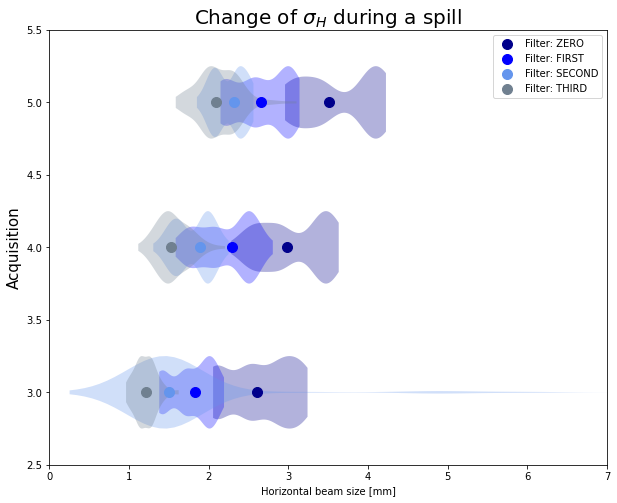
\includegraphics[width=\textwidth]{03_Empirical_Measurements/images/sigmaH.png}
        \caption{Horizontal beam size}
        \label{fig:sigmaH}
    \end{subfigure}
    \hfill
    \begin{subfigure}[b]{0.49\textwidth}
        \centering
        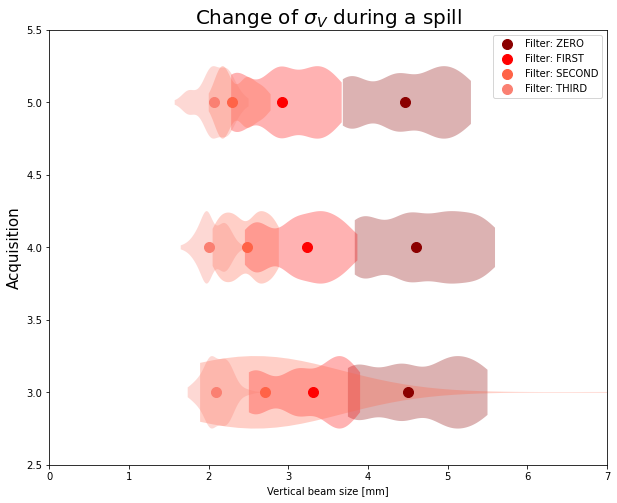
\includegraphics[width=\textwidth]{03_Empirical_Measurements/images/sigmaV.png}
        \caption{Horizontal beam size}
        \label{fig:sigmaV}
    \end{subfigure}
    \caption{Comparison of beam size during a spill average of 25 acquisitions.}
    \label{fig:filter_sigma}
\end{figure}

Figures \ref{fig:centroidH} and \ref{fig:centroidV} display the centroid in both planes across the different filters. Here, the filters are not critical for obtaining accurate beam position measurements, as expected. An additional relevant observation is that variations in intensity, either an increase or a decrease, can mitigate BTV saturation without influencing the beam size. This could be beneficial under certain experimental conditions.
\\

\begin{figure}[htbp]
    \centering
    \begin{subfigure}[b]{0.49\textwidth}
        \centering
        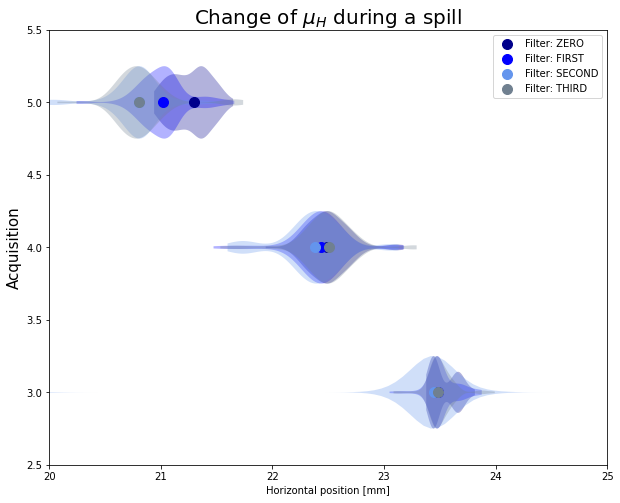
\includegraphics[width=\textwidth]{03_Empirical_Measurements/images/muH.png}
        \caption{Horizontal centroid}
        \label{fig:centroidH}
    \end{subfigure}
    \hfill
    \begin{subfigure}[b]{0.49\textwidth}
        \centering
        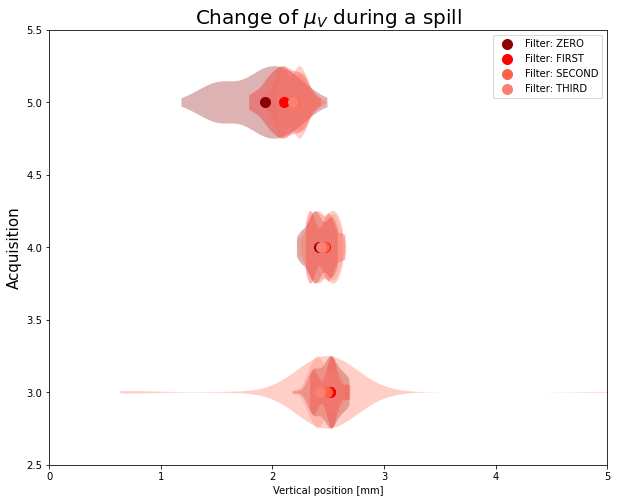
\includegraphics[width=\textwidth]{03_Empirical_Measurements/images/muV.png}
        \caption{Horizontal centroid}
        \label{fig:centroidV}
    \end{subfigure}
    \caption{Comparison of beam centroid during a spill average of 25 acquisitions.}
    \label{fig:filter_centroid}
\end{figure}

Accurate measurements of beam size, whether obtained through the use of filter wheels or alternative methods, are indispensable for precise determination of initial beam conditions. Previous use of saturated beam size data for MAD-X reconstruction has been found to yield inaccurate initial beam parameters. Therefore, ensuring the accuracy of beam size measurements is critical in for reliable beam characterization.
\\

\subsubsection{Image Processing Techniques}

To achieve precise beam size measurements using the BTVs, it is essential to apply image processing methods, given the inherent noise present in the raw image. The initial step involves processing the raw image through a sequence of a median filter and a Gaussian filter, which smooths neighboring pixels\footnote{Various filters such as bicubic interpolation and singular applications of either the median or Gaussian filter have been tested. However, for the present application, a sequential combination of the median filter followed by a Gaussian filter seems to be the most suitable.} and remove noise. This filtering step is succeeded by an initial Gaussian fit, used to estimate the beam center. The estimated beam size is then employed to create an elliptical mask, see Fig. \ref{fig:elliptical_mask}, facilitating the exclusion of regions far from the beam. Subsequently, a second Gaussian fit provides the final beam size measurement. Figure \ref{fig:image_processing} illustrates the enhancement in signal quality upon conducting these successive image processing steps.

\begin{figure}[htbp]
\centering
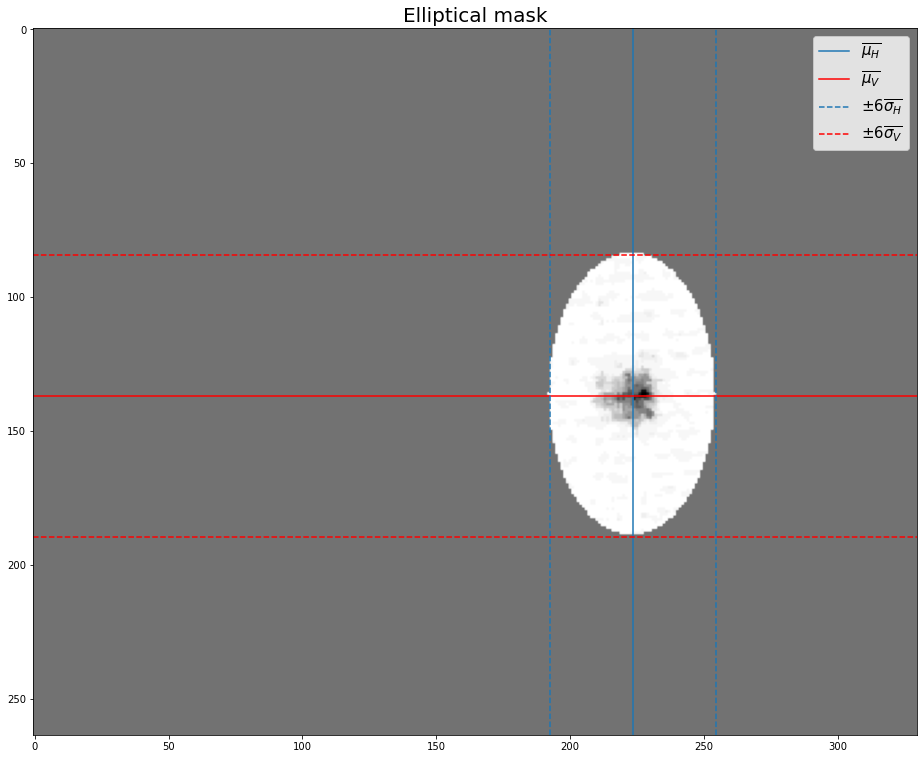
\includegraphics[width=0.7\textwidth]{03_Empirical_Measurements/images/elliptical_mask.png}
\caption{Elliptical mask applied to the processed BTV image, centered by using an initial gaussian fit with a multiple of $\sigma$ used for the dimension of the ellipse axis.}
\label{fig:elliptical_mask}
\end{figure}

\begin{figure}[htbp]
\centering
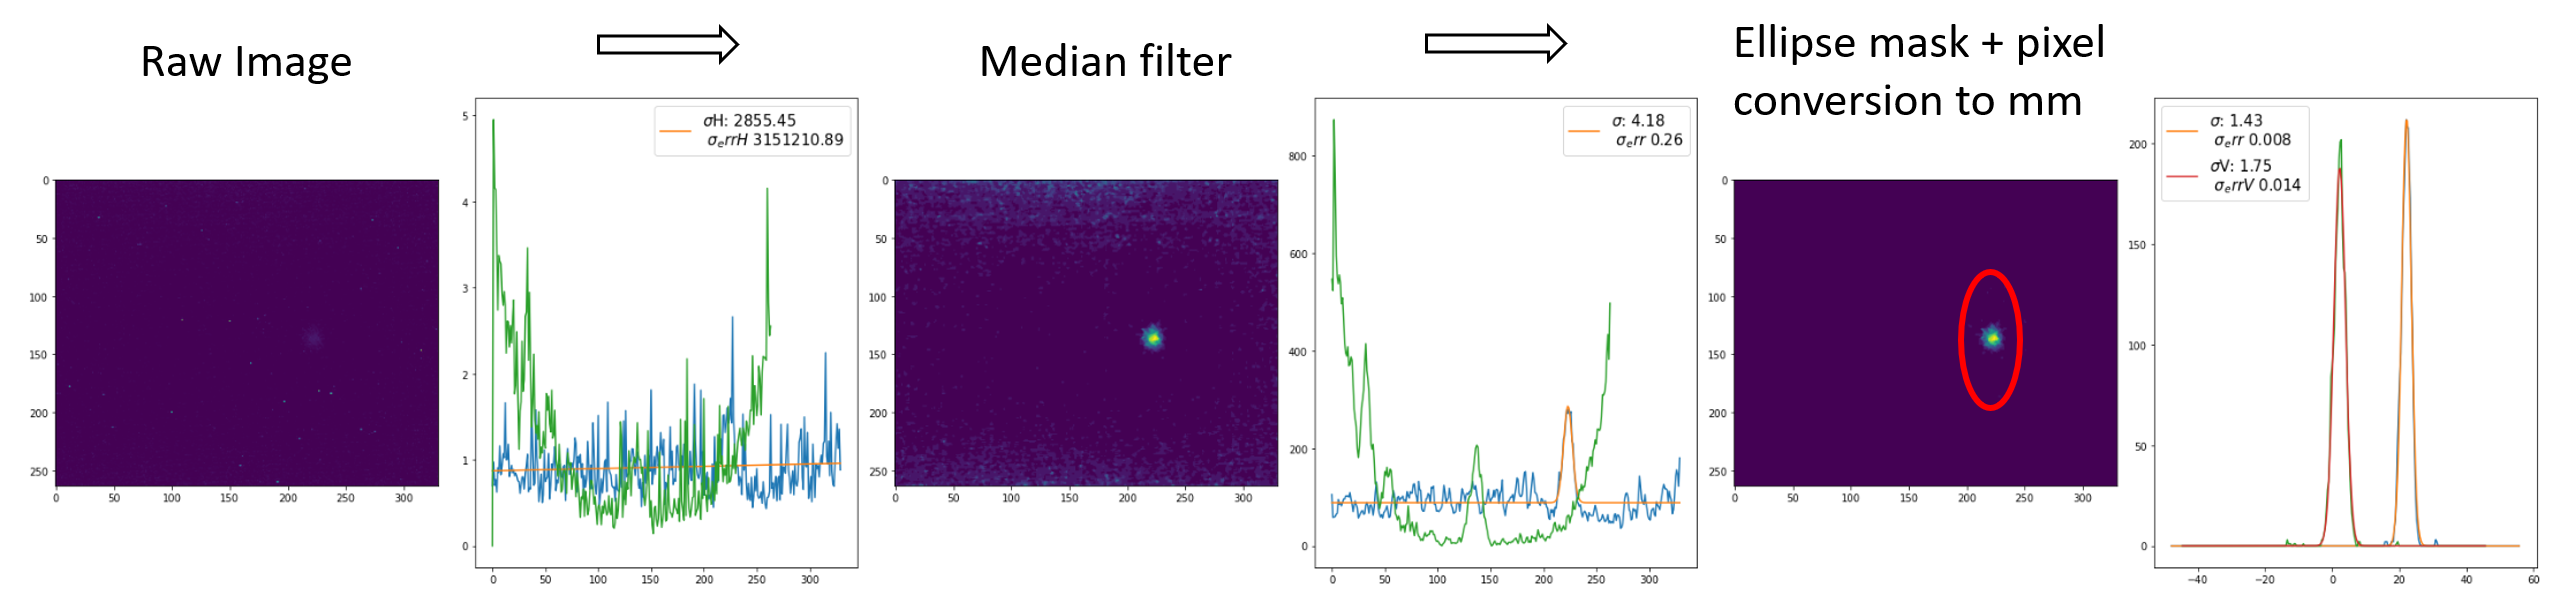
\includegraphics[width=\textwidth]{03_Empirical_Measurements/images/image_processing.png}
\caption{Illustration of signal quality improvement after consecutive image processing steps.}
\label{fig:image_processing}
\end{figure}

\subsubsection{Additional information on beam size measurement}

A few lessons are worth sharing to correctly reconstruct the initial parameters. In particular, one should carefully select the acquisition frame from the BTV so as to have a constant beam size. If it's at the edge of the spill, the beam might be cut because of the jitter in the acquisition. It is thus best to use an acquisition in the middle of the spill. Furthermore, the installation of filter wheels on the BTV is of invaluable to the reconstruction. Without filters, the fluorescent screen would saturate at high intensity which would give erroneous beam size measurements. Careful selection of the measurements from the quadrupole scan should be made. Combination of quadrupole at high and low strength might significantly alter the beam which could then scrap the apertures. Such measurement should be discarded. In general regions close to the minimum and maximum of the parabolas are sufficient. To speed up the optimisation algorithm an efficient way to prepare the measurement is to create a single data frame regrouping the parsed data with columns containing the quadrupole strength (K1s) and horizontal and vertical beam size.


\subsection{Transfer line initial condition reconstruction}

% This subsection should focus on how you identified the initial parameters for your study. Include the following points:
% A description of the parameters and their significance.
% The method used to determine these initial parameters.
% Any challenges faced and how you overcame them.
% The final list of initial parameters.

\subsection{Methodology}
The method to find the initial conditions of a transfer line using empirical measurements will now be described. First a set of quadrupole scan is collected by varying the strength (K1s) of a single or a combination of quadrupoles and measuring the beam size downstream of these modified optics. Different combination of quadrupole strength should be made and optimized to have as many as minimums and maximums (parabolic) beam size variation as possible. Once the measurements are done, an optimizer shall be ran on the MAD-X initial conditions of the transfer line starting with the closest guess to the initial conditions and calculating the beam sizes at the location of the instrument. A comparison between the measurement and simulation is made and minimized by iterating through the initial conditions. The iteration is done via an optimization library such as Scipy of Py-BOBYQA. A diagram of this technique is presented in Fig. \ref{fig:initial_condition_diagram}.
\\
\begin{figure}
    \centering
    \scalebox{0.8}{

\tikzset{every picture/.style={line width=0.75pt}} %set default line width to 0.75pt        

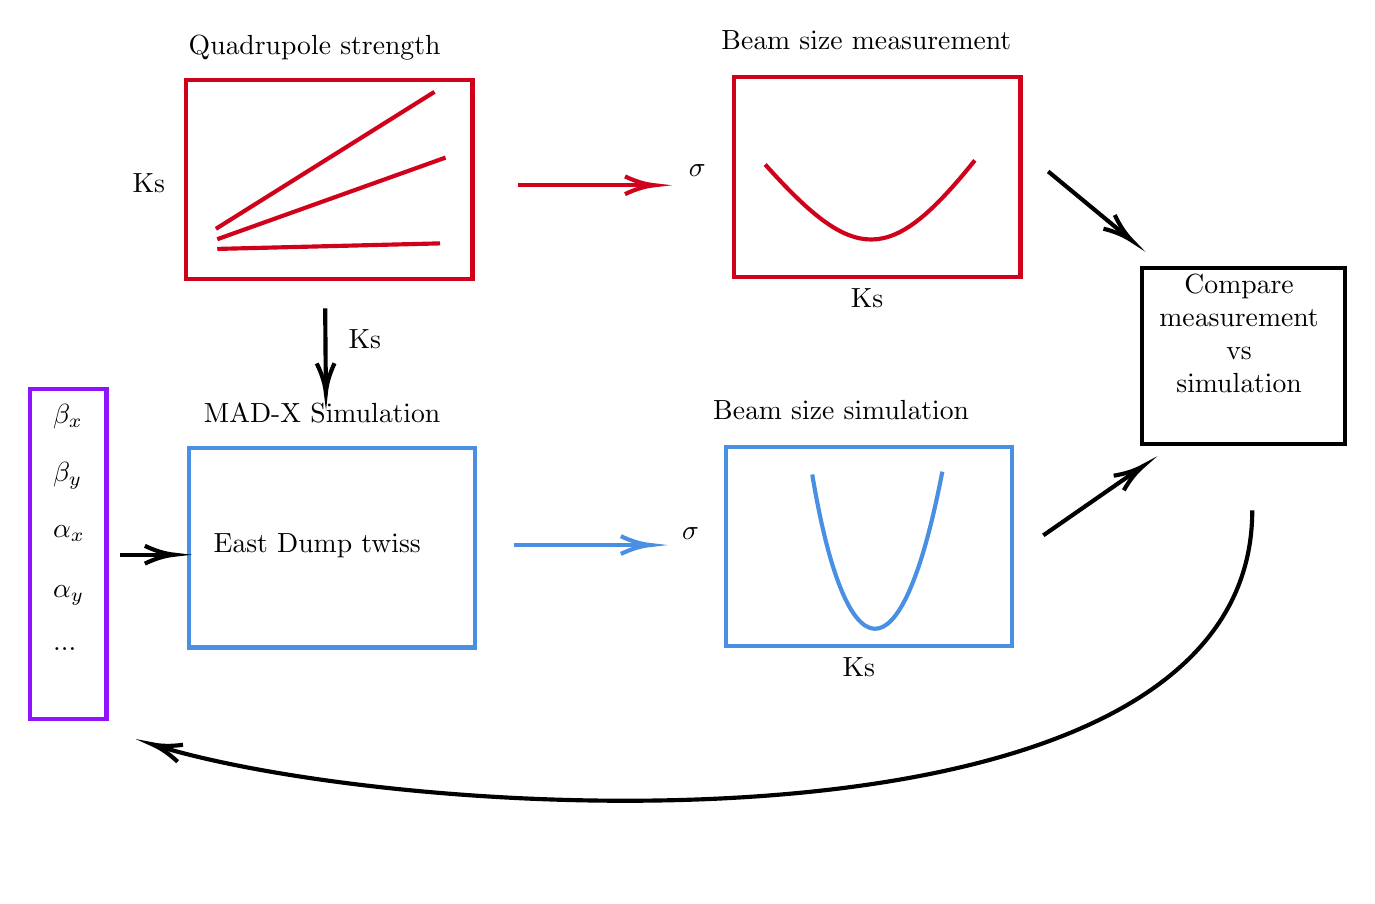
\begin{tikzpicture}[x=0.75pt,y=0.75pt,yscale=-1,xscale=1]
%uncomment if require: \path (0,480); %set diagram left start at 0, and has height of 480

%Shape: Rectangle [id:dp4246347329167801] 
\draw  [color={rgb, 255:red, 208; green, 2; blue, 27 }  ,draw opacity=1 ][line width=1.5]  (362.67,99.33) -- (500.67,99.33) -- (500.67,195.33) -- (362.67,195.33) -- cycle ;
%Curve Lines [id:da9888709896390471] 
\draw [color={rgb, 255:red, 208; green, 2; blue, 27 }  ,draw opacity=1 ][line width=1.5]    (377.67,141.33) .. controls (420.67,189.33) and (437.67,190.33) .. (478.67,139.33) ;
%Shape: Rectangle [id:dp49952149002749646] 
\draw  [color={rgb, 255:red, 208; green, 2; blue, 27 }  ,draw opacity=1 ][line width=1.5]  (98.67,100.67) -- (236.67,100.67) -- (236.67,196.67) -- (98.67,196.67) -- cycle ;
%Straight Lines [id:da9425896029593615] 
\draw [color={rgb, 255:red, 208; green, 2; blue, 27 }  ,draw opacity=1 ][line width=1.5]    (113,172.33) -- (218.33,106.33) ;
%Straight Lines [id:da0776144392613658] 
\draw [color={rgb, 255:red, 208; green, 2; blue, 27 }  ,draw opacity=1 ][line width=1.5]    (113.67,177.33) -- (223.67,138) ;
%Straight Lines [id:da02037742317127811] 
\draw [color={rgb, 255:red, 208; green, 2; blue, 27 }  ,draw opacity=1 ][line width=1.5]    (113.67,182) -- (221,179.33) ;
%Straight Lines [id:da070053405995959] 
\draw [color={rgb, 255:red, 208; green, 2; blue, 27 }  ,draw opacity=1 ][line width=1.5]    (258.67,151.33) -- (321.33,151.33) ;
\draw [shift={(324.33,151.33)}, rotate = 180] [color={rgb, 255:red, 208; green, 2; blue, 27 }  ,draw opacity=1 ][line width=1.5]    (14.21,-4.28) .. controls (9.04,-1.82) and (4.3,-0.39) .. (0,0) .. controls (4.3,0.39) and (9.04,1.82) .. (14.21,4.28)   ;
%Shape: Rectangle [id:dp944364271889234] 
\draw  [color={rgb, 255:red, 144; green, 19; blue, 254 }  ,draw opacity=1 ][line width=1.5]  (23.33,249.33) -- (60.33,249.33) -- (60.33,408.67) -- (23.33,408.67) -- cycle ;
%Straight Lines [id:da8395245156263087] 
\draw [color={rgb, 255:red, 0; green, 0; blue, 0 }  ,draw opacity=1 ][line width=1.5]    (165.67,210.67) -- (165.98,248.33) ;
\draw [shift={(166,251.33)}, rotate = 269.53] [color={rgb, 255:red, 0; green, 0; blue, 0 }  ,draw opacity=1 ][line width=1.5]    (14.21,-4.28) .. controls (9.04,-1.82) and (4.3,-0.39) .. (0,0) .. controls (4.3,0.39) and (9.04,1.82) .. (14.21,4.28)   ;
%Shape: Rectangle [id:dp4855606702968256] 
\draw  [color={rgb, 255:red, 74; green, 144; blue, 226 }  ,draw opacity=1 ][line width=1.5]  (100,278) -- (238,278) -- (238,374) -- (100,374) -- cycle ;
%Straight Lines [id:da7022632349262303] 
\draw [line width=1.5]    (66.67,329.33) -- (90,329.33) ;
\draw [shift={(93,329.33)}, rotate = 180] [color={rgb, 255:red, 0; green, 0; blue, 0 }  ][line width=1.5]    (14.21,-4.28) .. controls (9.04,-1.82) and (4.3,-0.39) .. (0,0) .. controls (4.3,0.39) and (9.04,1.82) .. (14.21,4.28)   ;
%Straight Lines [id:da3968621494939437] 
\draw [color={rgb, 255:red, 74; green, 144; blue, 226 }  ,draw opacity=1 ][line width=1.5]    (256.67,324.67) -- (319.33,324.67) ;
\draw [shift={(322.33,324.67)}, rotate = 180] [color={rgb, 255:red, 74; green, 144; blue, 226 }  ,draw opacity=1 ][line width=1.5]    (14.21,-4.28) .. controls (9.04,-1.82) and (4.3,-0.39) .. (0,0) .. controls (4.3,0.39) and (9.04,1.82) .. (14.21,4.28)   ;
%Shape: Rectangle [id:dp4118518001915987] 
\draw  [color={rgb, 255:red, 74; green, 144; blue, 226 }  ,draw opacity=1 ][line width=1.5]  (358.67,277.33) -- (496.67,277.33) -- (496.67,373.33) -- (358.67,373.33) -- cycle ;
%Curve Lines [id:da2553267141266382] 
\draw [color={rgb, 255:red, 74; green, 144; blue, 226 }  ,draw opacity=1 ][line width=1.5]    (400.33,290.67) .. controls (416.33,386.67) and (443,393.33) .. (463,289.33) ;
%Shape: Rectangle [id:dp8890861260646525] 
\draw  [line width=1.5]  (559.33,191.33) -- (657,191.33) -- (657,276) -- (559.33,276) -- cycle ;
%Curve Lines [id:da18599849782409872] 
\draw [line width=1.5]    (612.33,308) .. controls (612.33,483.12) and (203.78,458.25) .. (84.12,421.23) ;
\draw [shift={(82.33,420.67)}, rotate = 17.65] [color={rgb, 255:red, 0; green, 0; blue, 0 }  ][line width=1.5]    (14.21,-4.28) .. controls (9.04,-1.82) and (4.3,-0.39) .. (0,0) .. controls (4.3,0.39) and (9.04,1.82) .. (14.21,4.28)   ;
%Straight Lines [id:da014820791284121837] 
\draw [line width=1.5]    (511.67,320) -- (557.2,288.38) ;
\draw [shift={(559.67,286.67)}, rotate = 145.22] [color={rgb, 255:red, 0; green, 0; blue, 0 }  ][line width=1.5]    (14.21,-4.28) .. controls (9.04,-1.82) and (4.3,-0.39) .. (0,0) .. controls (4.3,0.39) and (9.04,1.82) .. (14.21,4.28)   ;
%Straight Lines [id:da7493093229877397] 
\draw [line width=1.5]    (514,144.67) -- (552.02,176.09) ;
\draw [shift={(554.33,178)}, rotate = 219.57] [color={rgb, 255:red, 0; green, 0; blue, 0 }  ][line width=1.5]    (14.21,-4.28) .. controls (9.04,-1.82) and (4.3,-0.39) .. (0,0) .. controls (4.3,0.39) and (9.04,1.82) .. (14.21,4.28)   ;

% Text Node
\draw (417.67,199.83) node [anchor=north west][inner sep=0.75pt]   [align=left] {Ks};
% Text Node
\draw (339.67,140.33) node [anchor=north west][inner sep=0.75pt]   [align=left] {$\displaystyle \sigma $};
% Text Node
\draw (71.67,144.5) node [anchor=north west][inner sep=0.75pt]   [align=left] {Ks};
% Text Node
\draw (98.67,77.67) node [anchor=north west][inner sep=0.75pt]   [align=left] {Quadrupole strength};
% Text Node
\draw (355.33,75.67) node [anchor=north west][inner sep=0.75pt]   [align=left] {Beam size measurement};
% Text Node
\draw (33.33,255.4) node [anchor=north west][inner sep=0.75pt]    {$\beta _{x}$};
% Text Node
\draw (33.33,283.4) node [anchor=north west][inner sep=0.75pt]    {$\beta _{y}$};
% Text Node
\draw (33.33,314.07) node [anchor=north west][inner sep=0.75pt]    {$\alpha _{x}$};
% Text Node
\draw (33.33,342.73) node [anchor=north west][inner sep=0.75pt]    {$\alpha _{y}$};
% Text Node
\draw (33.33,372.73) node [anchor=north west][inner sep=0.75pt]    {$...$};
% Text Node
\draw (106,255) node [anchor=north west][inner sep=0.75pt]   [align=left] {MAD-X Simulation};
% Text Node
\draw (110.67,317.67) node [anchor=north west][inner sep=0.75pt]   [align=left] {East Dump twiss};
% Text Node
\draw (413.67,377.83) node [anchor=north west][inner sep=0.75pt]   [align=left] {Ks};
% Text Node
\draw (336.33,315) node [anchor=north west][inner sep=0.75pt]   [align=left] {$\displaystyle \sigma $};
% Text Node
\draw (351.33,253.67) node [anchor=north west][inner sep=0.75pt]   [align=left] {Beam size simulation};
% Text Node
\draw (561.33,193) node [anchor=north west][inner sep=0.75pt]   [align=left] {\begin{minipage}[lt]{65.09pt}\setlength\topsep{0pt}
\begin{center}
Compare\\measurement\\vs\\simulation
\end{center}

\end{minipage}};
% Text Node
\draw (175.67,219.83) node [anchor=north west][inner sep=0.75pt]   [align=left] {Ks};

\end{tikzpicture}
}
    \caption{Initial condition diagram}
    \label{fig:initial_condition_diagram}
\end{figure}

\subsubsection{Result of the optimization}

Figure \ref{fig:combined_measurements} shows the four quadrupole scan measurement used to determine the initial conditions as well as the MAD-X predictions using the initial conditions that it converged on. The right side of the figure shows the combination of current applied where each measurement was repeated five times.
\\

\begin{figure}[htbp]
\centering
\includegraphics[width=0.7\textwidth]{03_Empirical_Measurements/images/combine_quadrupole_scan_east_dump.png}
\caption{Quadrupole scan to the East Dump compared to the MAD-X prediction using the inital conditions found through optimization. The x-scale on the left side of the figure is labeled K1 QFN01 to present the data on a plot but the three quadrupole were modified during the scan.}
\label{fig:combined_measurements}
\end{figure}

It is expected that the measurement and simulation with the East Dump will be close as they were optimized on and the East Dump line is a short line with only a few quadrupole. Of particular interested would be to assess how accurate the MAD-X model is through the main lines in the East Area where no measurement. Figure \ref{fig:comparison_btv96} show how the model predicts the minimums and maximums in beam size at BTV96 located in CHARM at the end of the T8 line. The absolute beam size measurement is however underestimated. An offset is observed in both planes where the measurements are slightly larger. This emittance mismatch can be explained by the large amount of air present in the transfer line in particular in the IRRAD experimental area which would effectively increase the emittances. Nevertheless, this first iteration of the method of using a parallel and short transfer line (East Dump 35 m) to predict the T8 line (135 m) with five additional quadrupoles and dipole can be used to make informed decisions about the optics of the line.

\begin{figure}[htbp]
\centering
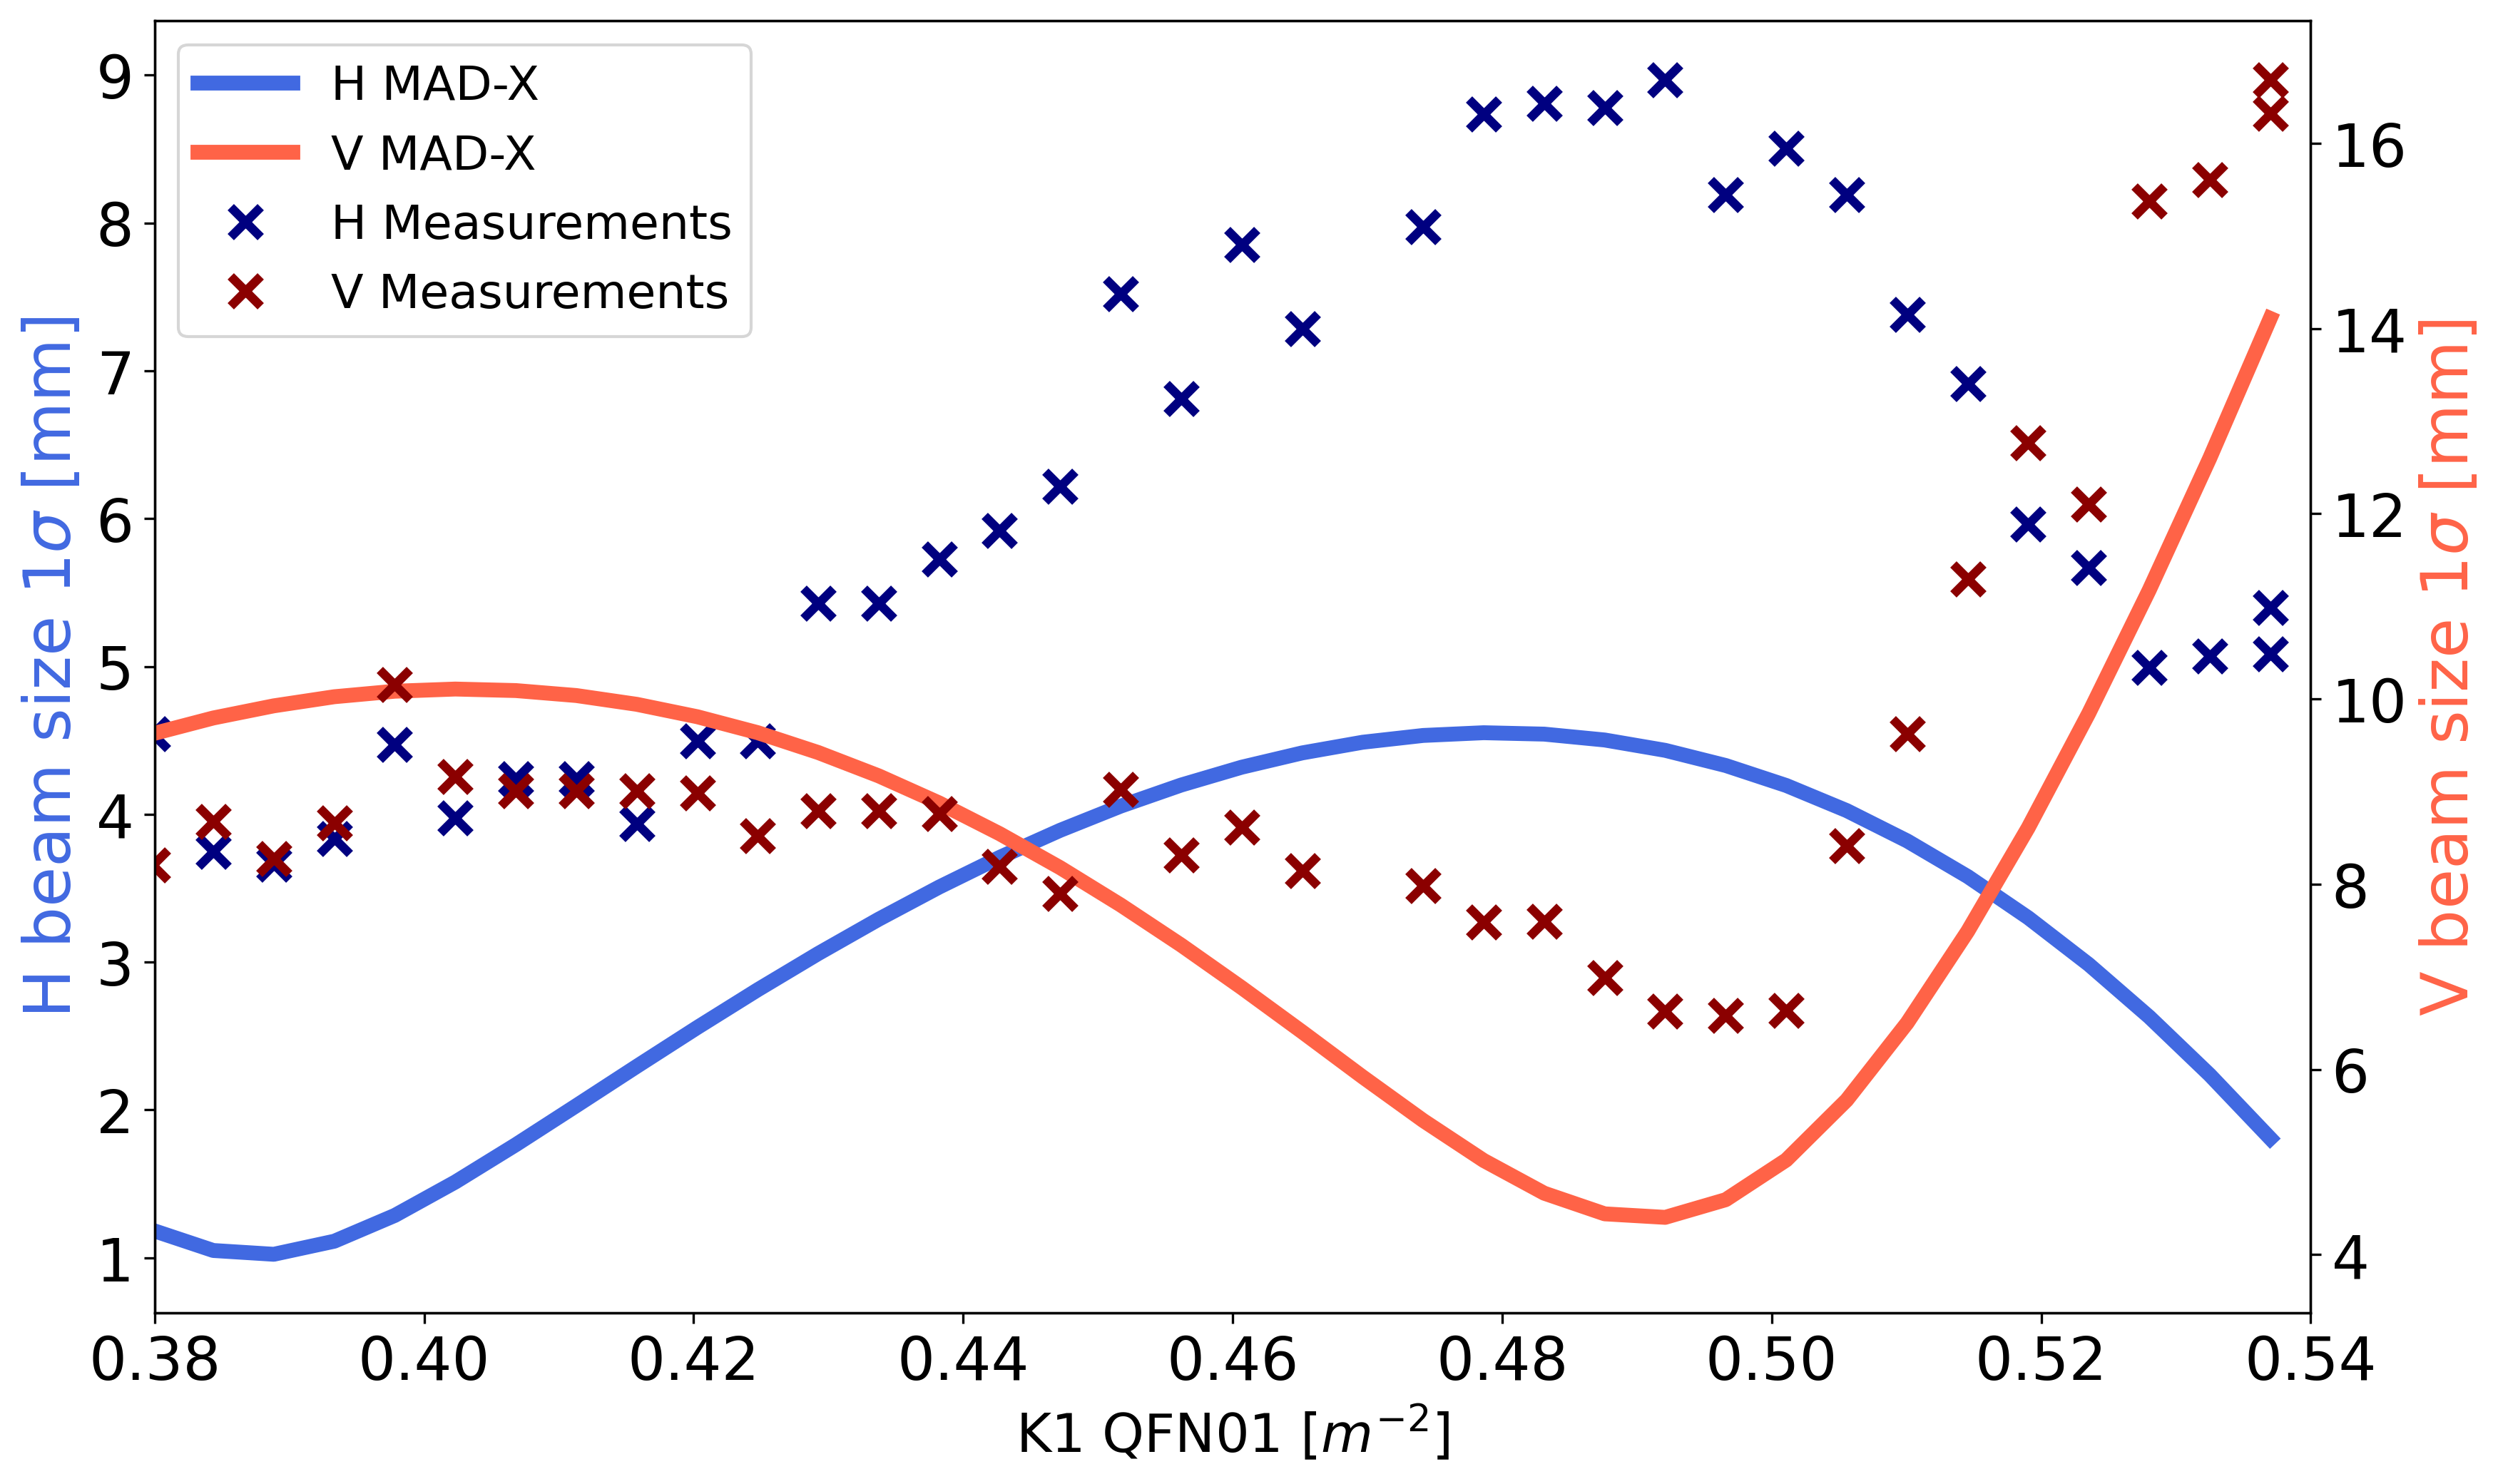
\includegraphics[width=0.7\textwidth]{03_Empirical_Measurements/images/east_quad_scan_df_meas_btv96.pickle.png}
\caption{Comparison between MAD-X model and beam size measurement in the CHARM area.}
\label{fig:comparison_btv96}
\end{figure}


\newpage
\subsubsection{Initial beam parameters of the East Area slow extracted beam}
\label{initial beam parameters empirical}

The initial parameters located upstream of the first quadrupole of the transfer line (Q74) are presented in Table \ref{table:beam_parameters_1} and \ref{table:beam_parameters_2}.


\begin{table}[htbp]
\centering
\caption{Initial Beam Parameters - Part 1}
\label{table:beam_parameters_1}
\begin{tabular}{|c|c|c|c|c|c|c|c|}
\hline
$\beta_{x}$ [m] & $\beta_{y}$ [m] & $\alpha_{x}$ & $\alpha_{y}$ & $D_{x}$ [m] & $D_{y}$ [m] & $D^{'}_{x}$[mrad] & $D^{'}_{y}$[mrad] \\
\hline
154.1 & 5.22 & -36.9 & 0.25 & 0.13 & 0.0 & 0.02 & 0.0 \\
\hline
\end{tabular}
\end{table}

\begin{table}[htbp]
\centering
\caption{Initial Beam Parameters - Part 2}
\label{table:beam_parameters_2}
\begin{tabular}{|c|c|c|}
\hline
$e_{xn}$ [m] & $e_{yn}$ [m] & $\frac{\Delta p}{p}$ \\
\hline
7.64e-06 & 3.53e-06 & 6.79e-4 \\
\hline
\end{tabular}
\end{table}


\subsection{EAST Area T8 optics 2023}

% For this part, you should describe:
% The reason for implementing new optics to the EAST area.
% The method used for this implementation and the considerations taken into account.
% The result of this new implementation, emphasizing the alignment with the initial parameters.

\subsubsection{Reasons for implementing new optics to the East Area}

The optics used during 2021 and 2022 in the T8 line needed to be modified as a large "tail", see Fig. \ref{fig:tail_irrad} was present in the horizontal plane which isn't ideal for the irradiation operations in IRRAD.
\\

\begin{figure}[H]
\centering
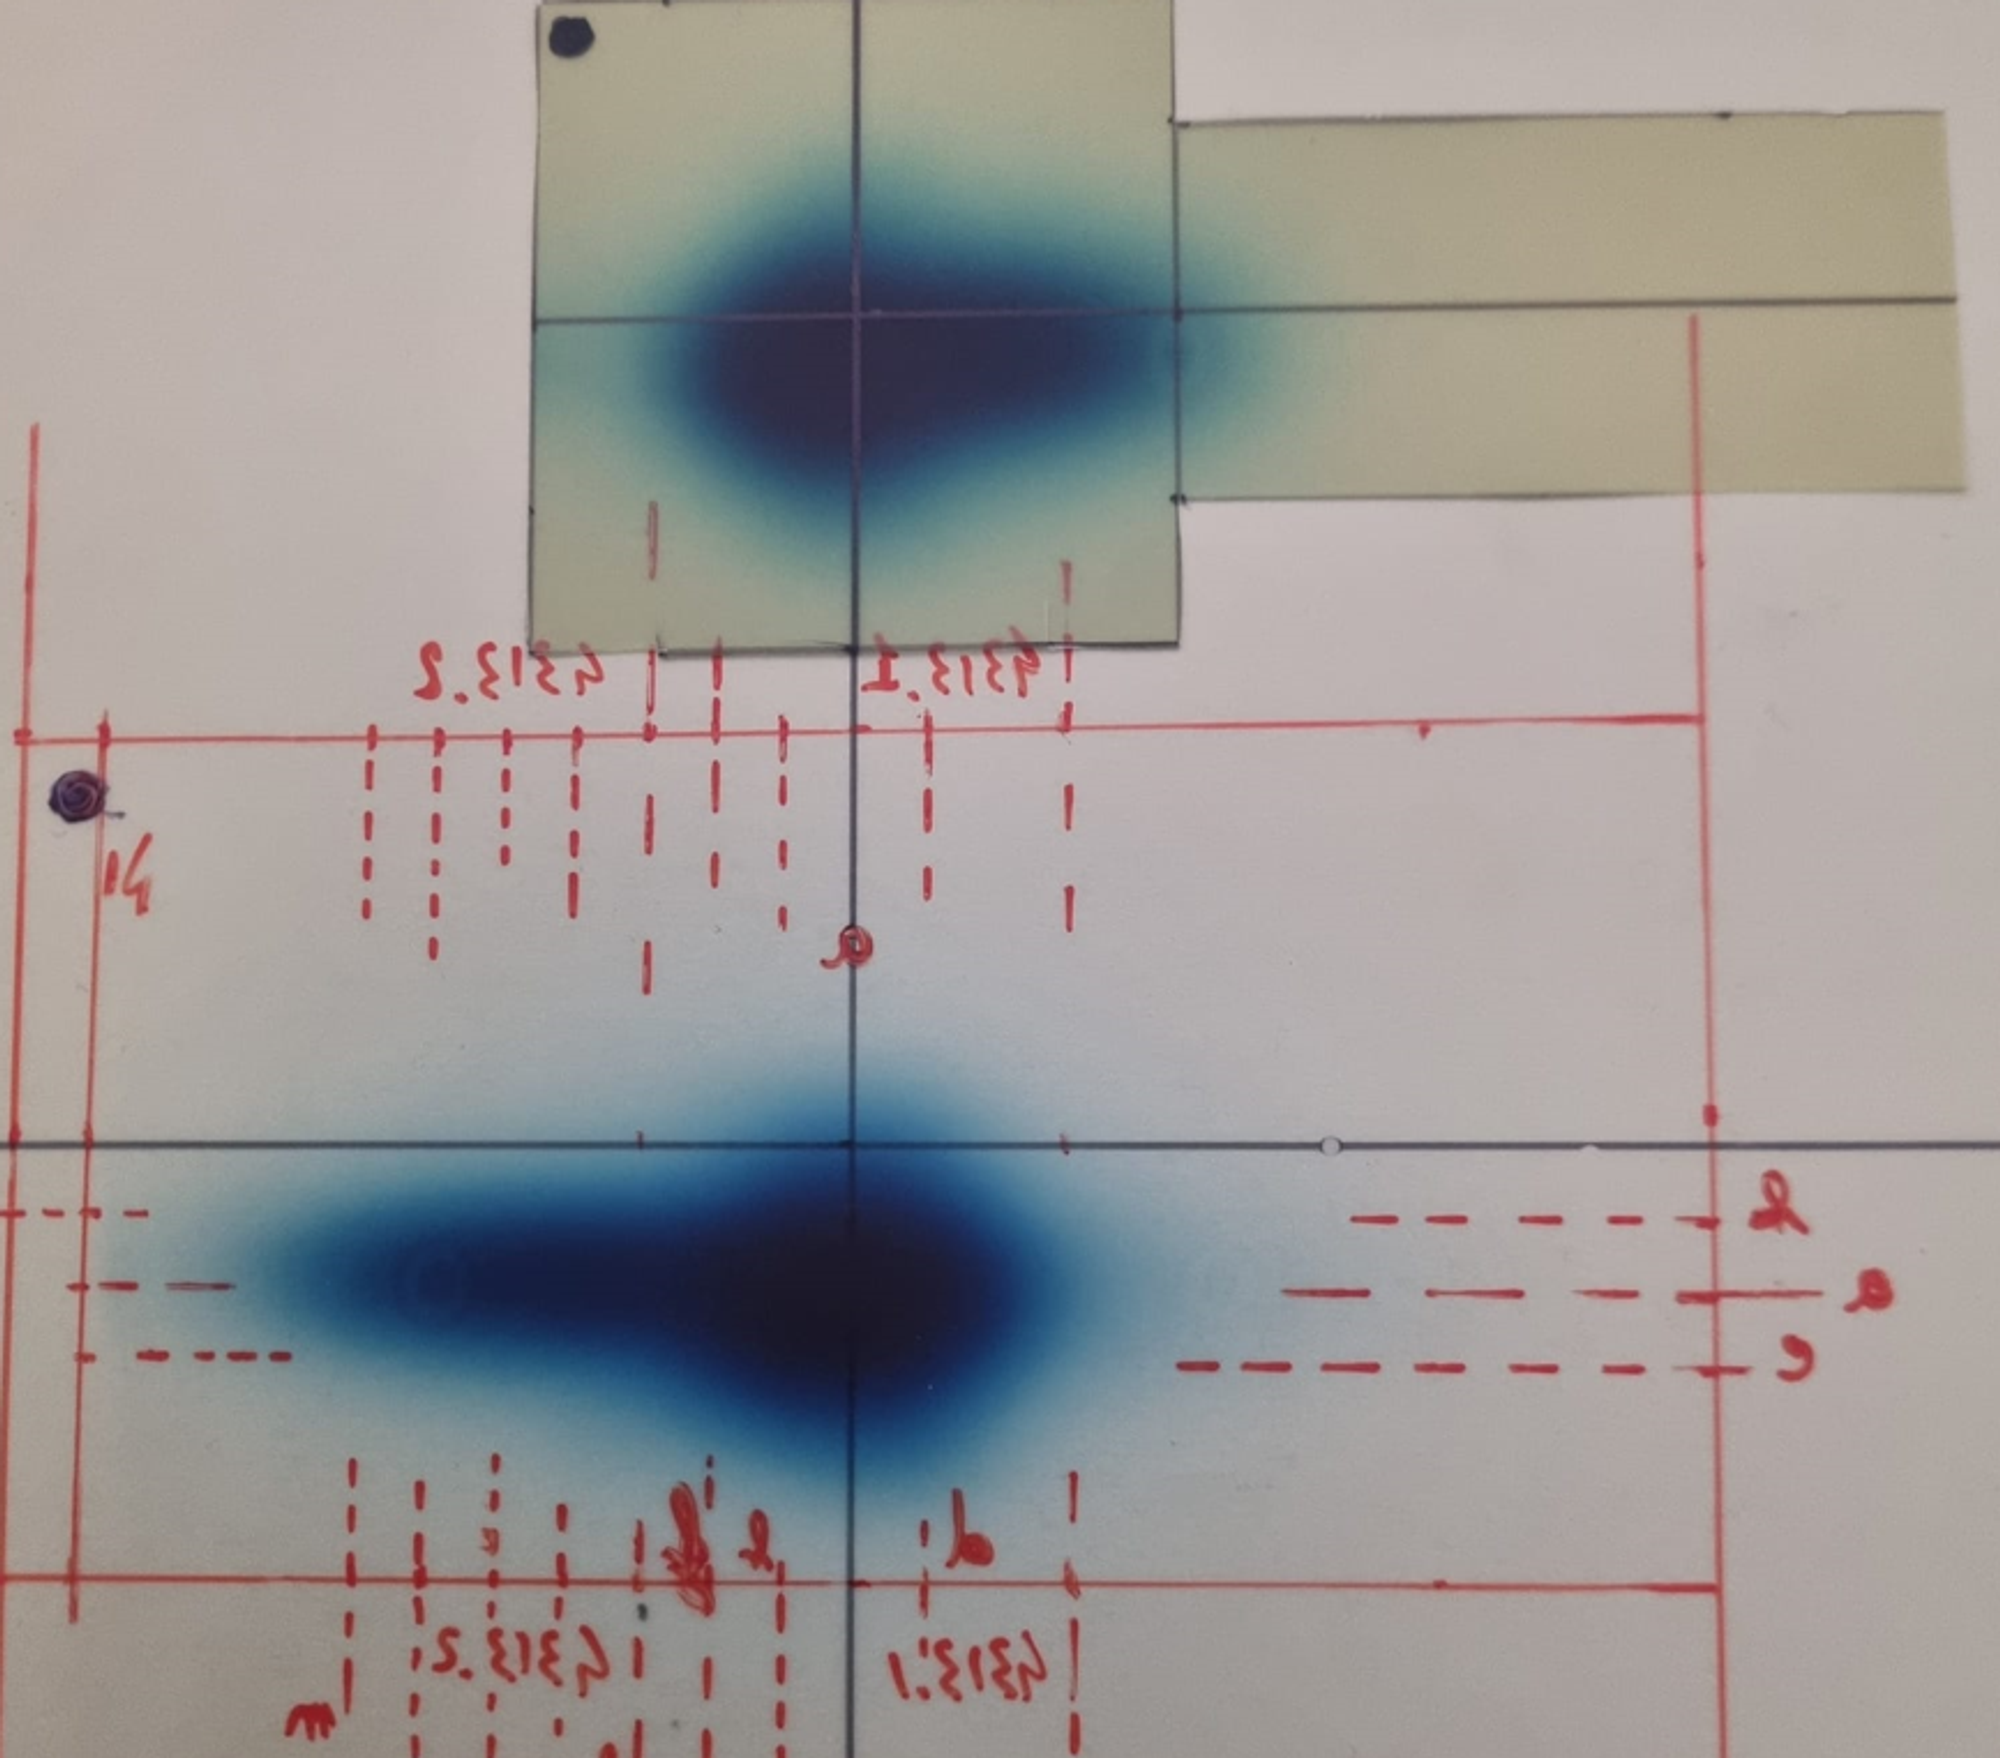
\includegraphics[width=0.6\textwidth]{03_Empirical_Measurements/images/tail_irrad.png}
\caption{GAFchromic film in IRRAD showing the "tail" before (bottom) and after (top) using the horizontal dipole corrector.}
\label{fig:tail_irrad}
\end{figure}

The tail is caused by the natural sweep due to an non-constant optics that starts in the PS ring and that propagate (and becomes larger) in the transfer line. This is particularly observed and unwanted in IRRAD that need symmetric round and parallel beams across there four irradiation stations. Initial hypothesis if dispersion in this region could cause asymmetric beam. While it is true that the dispersion is non-zero and non-linear at the IRRAD irradiation stations which could produce a tail, see Fig. \ref{fig:nonlinear_dispersion}, PTC simulation show, see Fig. \ref{fig:PTC_dispersion}, that to reproducing these tails require an offset in momentum of 3\% which is orders of magnitude away from the real beam momentum spread which is closer to 0.03\% $\frac{\Delta p}{p}$.

\begin{figure}[htbp]
\centering
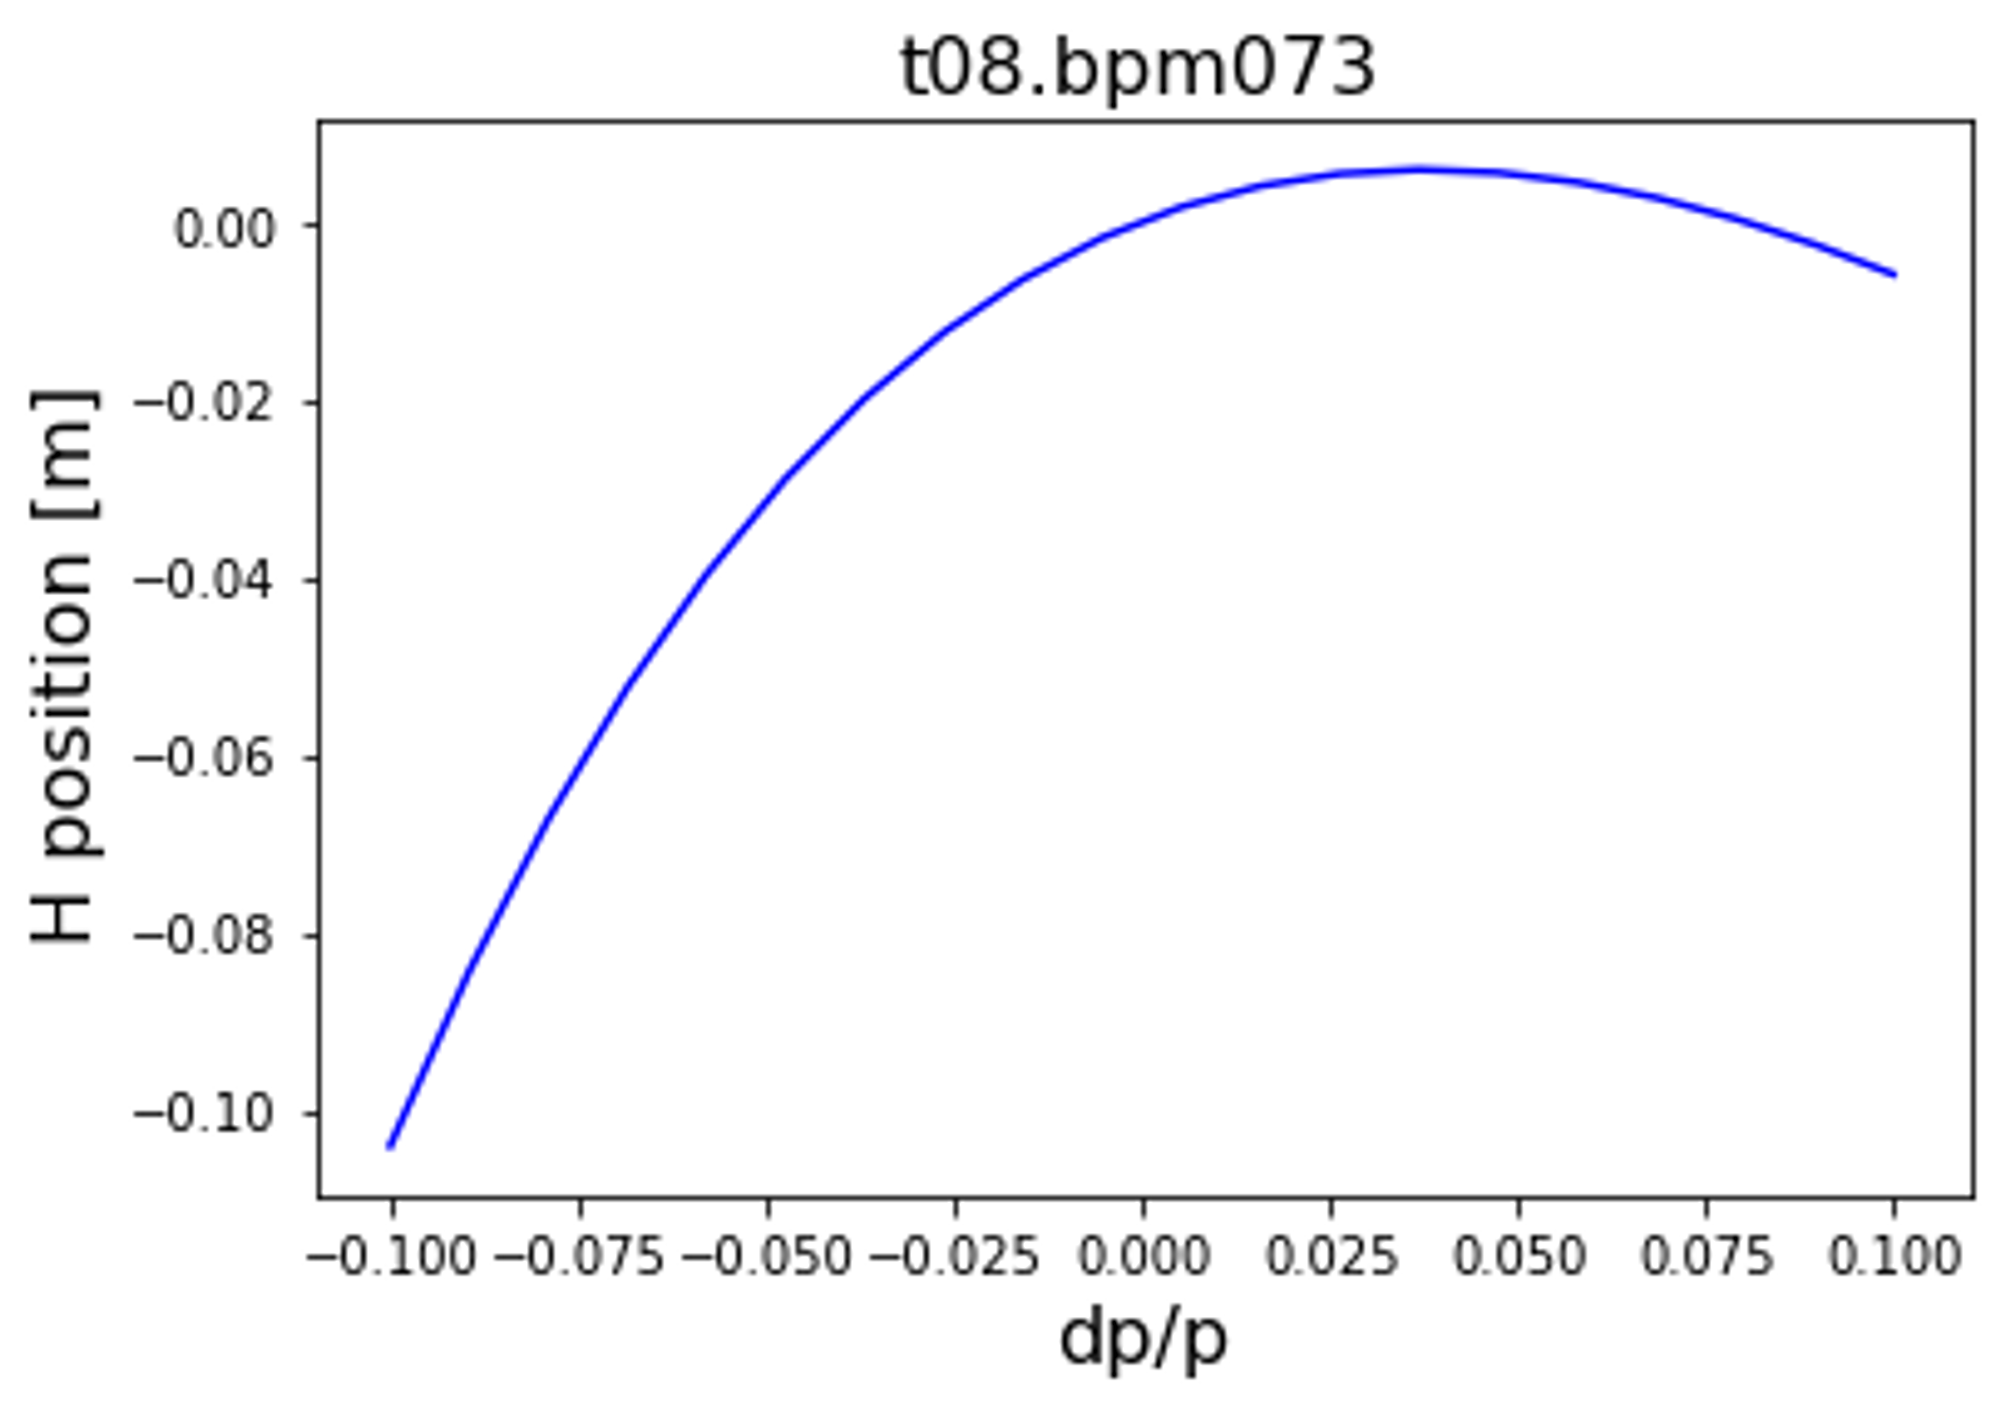
\includegraphics[width=0.5\textwidth]{03_Empirical_Measurements/images/nonlinear_dispersion.png}
\caption{Non-linear dispersion at IRRAD BPM1.}
\label{fig:nonlinear_dispersion}
\end{figure}

\begin{figure}[htbp]
\centering
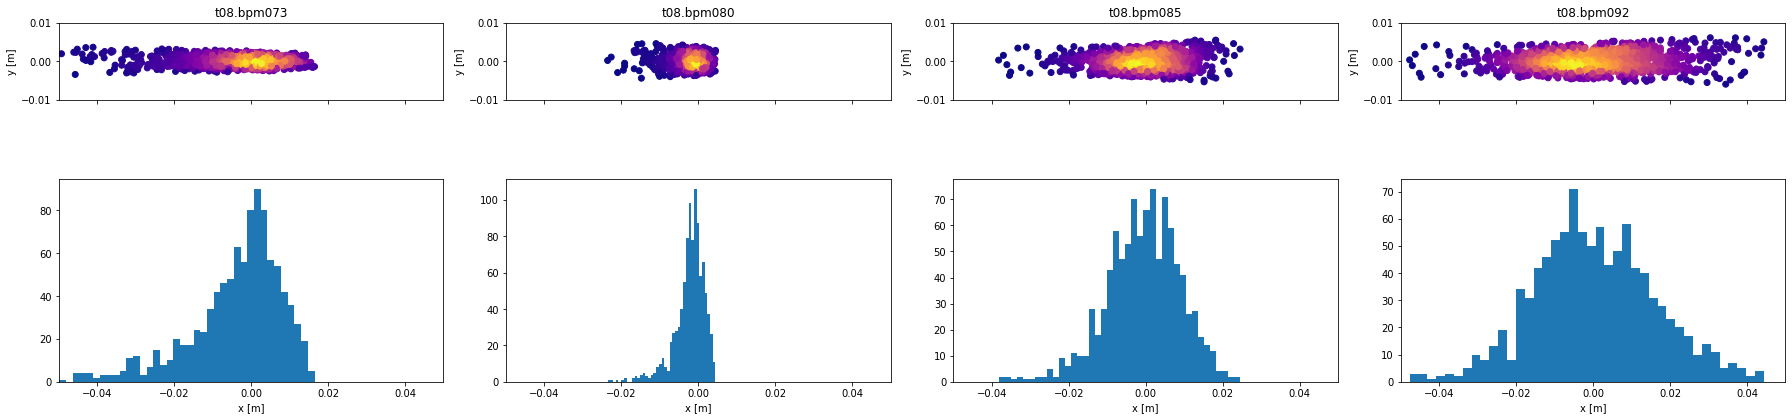
\includegraphics[width=1.0\textwidth]{03_Empirical_Measurements/images/dispersion_3percent_dpp.png}
\caption{PTC simulation of the beam distribution in real space at the IRRAD BPMs location.}
\label{fig:PTC_dispersion}
\end{figure}

Knowing that the tail was only produced by the sweep, a linear ramp on a horizontal corrector magnet was set-up to cancel it. This indeed lowered the amount of tail but also changed it's side which means we crossed a focal point. However as there are no instrumentation capable of producing multiple acquisitions during a single spill at the irradiation point it is difficult to cancel the tail through this method.

\subsubsection{Methodology for Implementing New Optics and Key Considerations}

The methodology for implementing the new optics was guided by the requisites and constraint from the IRRAD team, using the MAD-X model of the line in tandem with an optimiser. The key specifications revolved around achieving an 13mm $\times$ 13.6mm full-width half-maximum (FWHM) beam, both symmetric and parallel across the four irradiation zones. A MAD-X model of the beam was used and optimized with these given constraints to produce new optics using the eight quadrupoles available in F61 and T8 and the initial conditions from Table \ref{table:beam_parameters_1} and \ref{table:beam_parameters_2}.
\\

Fast iterations were made possible by using a script that uploads the newly produces optics to the CCC computers, followed by setting them using Py-Japc. Iterations were necessary due to the observed divergence between the model and the real-world measurements; particularly, the model does not perfectly predict the absolute beam size, notably in the CHARM area, the second irradiation area and the most downstream part of the transfer line.
\\

As a result, the optics optimizer didn't actually use the specified constrained but rather values close to it so that the actually beam would match the specifications. Additionally, it was noticed that large changes to the most upstream quadrupoles (Q74L, specifically, being close to the stray fields) degraded heavily the beam. To circumvent this issue, only minor modifications were applied to these upstream quadrupoles --- within a few percent, whereas the quadrupoles in closer proximity to the irradiation area were permitted a full range of strength variation.
\\

This model-informed iterative approach considerably expedited the process, enabling the implementation of new optics within a few hours. The incorporation of an air scattering model may further enhance the accuracy and precision of the model, facilitating changes in the optics even further.


\subsubsection{Results of the new optics implementation}

After a few iterations, a satisfactory new optics was selected for the T8 line. Table \ref{table:New optics quadrupole strenghts} presents the quadrupole strengths of the optics implemented in April 2023 for the T8 line.

\begin{table}[htbp]
    \centering
    \caption{Quadrupole Strengths}
    \begin{tabular}{cc}
        \hline
        Quadrupole & K1 [$\text{m}^{-2}$] \\
        \hline
        kQFN1 & 0.49169 \\
        kQDN2 & -0.18725 \\
        kQFN3 & 0.2142 \\
        kQDN4 & -0.07838 \\
        kQFN5 & 0.1877 \\
        kQDN6 & -0.1922 \\
        kQDN7 & -0.07342 \\
        kQFN8 & 0.06299 \\
        \hline
    \end{tabular}
    \label{table:New optics quadrupole strenghts}
\end{table}

The comparison between the simulation and experimental measurements is depicted in Figure \ref{fig:IRRAD_new_optics_sim_meas_comparison}. The blue curve denotes the simulation results for the one sigma horizontal beam size, while the red curve represents the vertical beam size. Markers have been added at the locations of the IRRAD BPMs to show beam size measurements averaged over a few hours (09:41 to 12:00 20/04/2023). A notable degree of conformity is observed in both planes, with a markedly good agreement in the vertical plane. The error bars, symbolizing the standard deviation for the beam size measurements, appear larger in the horizontal plane.

\begin{figure}[htbp]
\centering
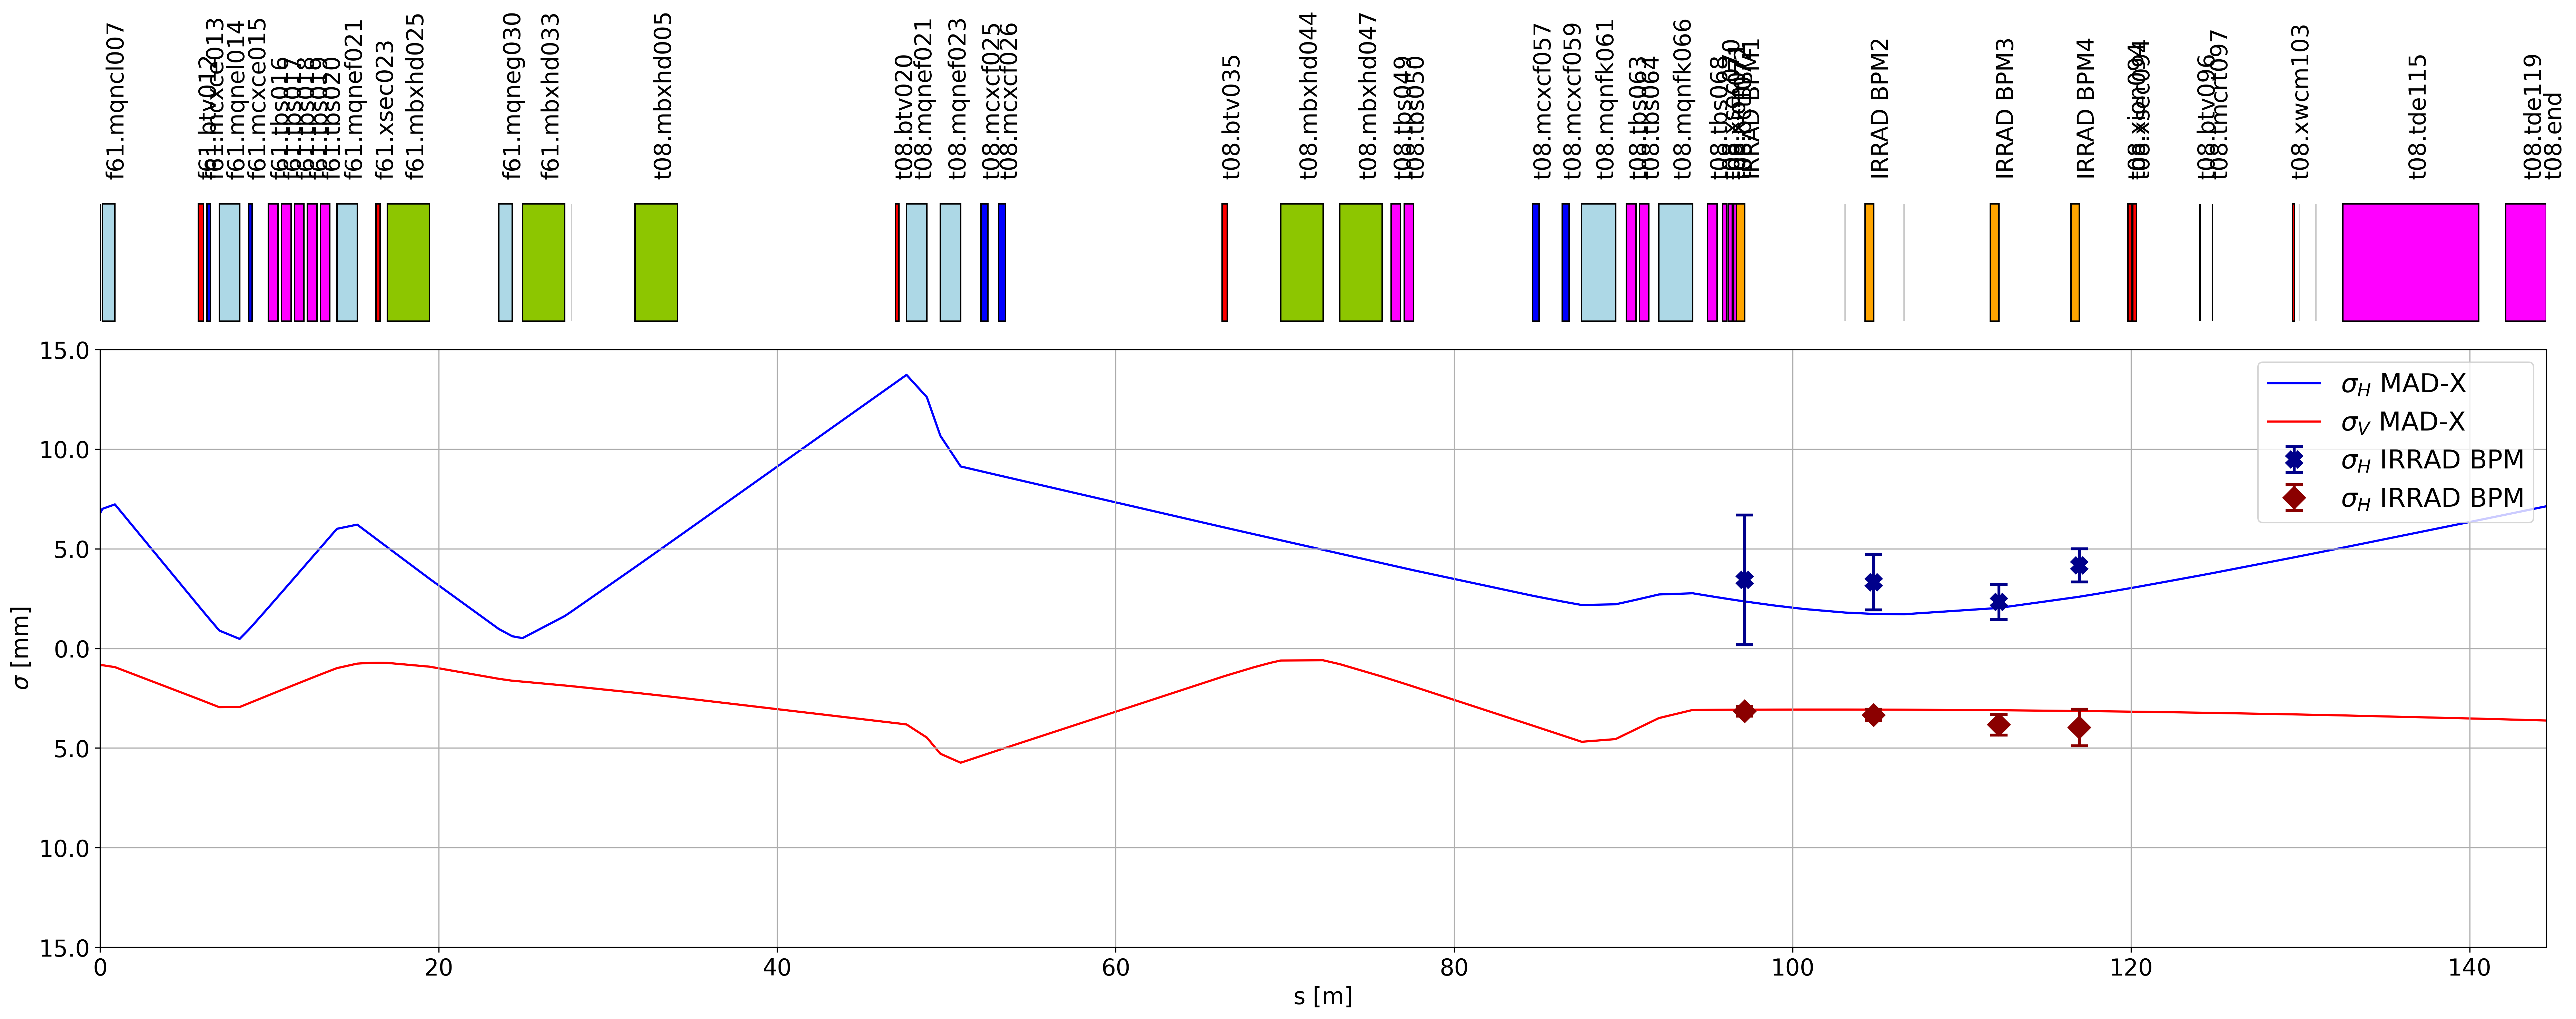
\includegraphics[width=1.0\textwidth]{03_Empirical_Measurements/images/t8_optics_with_measurement_zoom.png}
\caption{Comparison between the MAD-X model of the T8 line and the measurements at the IRRAD BPMs.}
\label{fig:IRRAD_new_optics_sim_meas_comparison}
\end{figure}

Figure \ref{fig:error_irrad_sim} shows the difference between the measurements and the simulation. It appears that the simulation under estimates the real beam size in a constant manner. In the horizontal plane the disagreement comes close to -50\% for BPM2. In the vertical plane the agreement is better. One however observes a trend in increase in disagreement which might be associated with emittance blowup due to air scattering.

\begin{figure}[htbp]
\centering
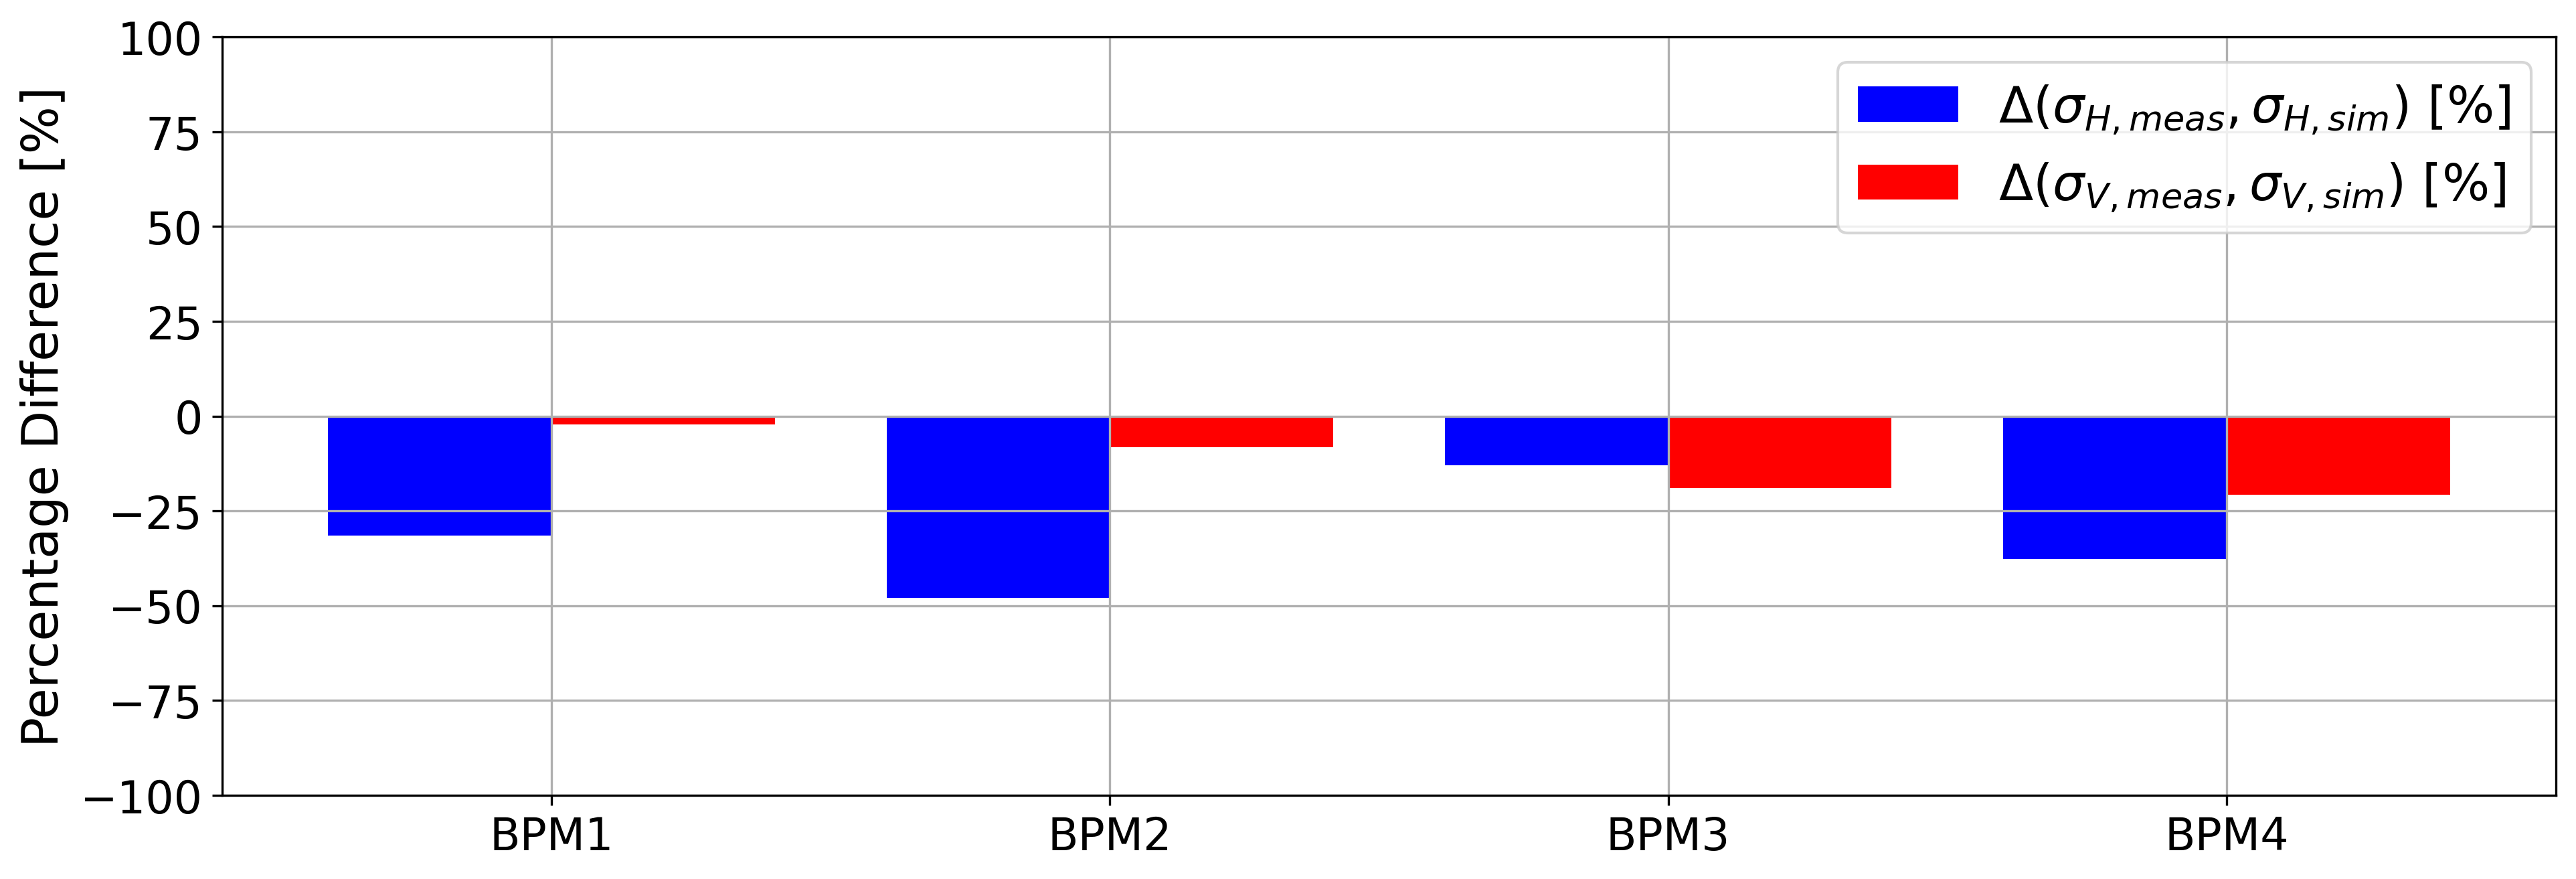
\includegraphics[width=0.9\textwidth]{03_Empirical_Measurements/images/percentage_diff_btw_sigma_meas_and_sim.png}
\caption{Percentage difference between beam size measurement median and simulation}
\label{fig:error_irrad_sim}
\end{figure}

% Figure \ref{fig:irrad_bpms_new_optics} shows the signal on the IRRAD BPMs.

% \begin{figure}[htbp]
% \centering
% 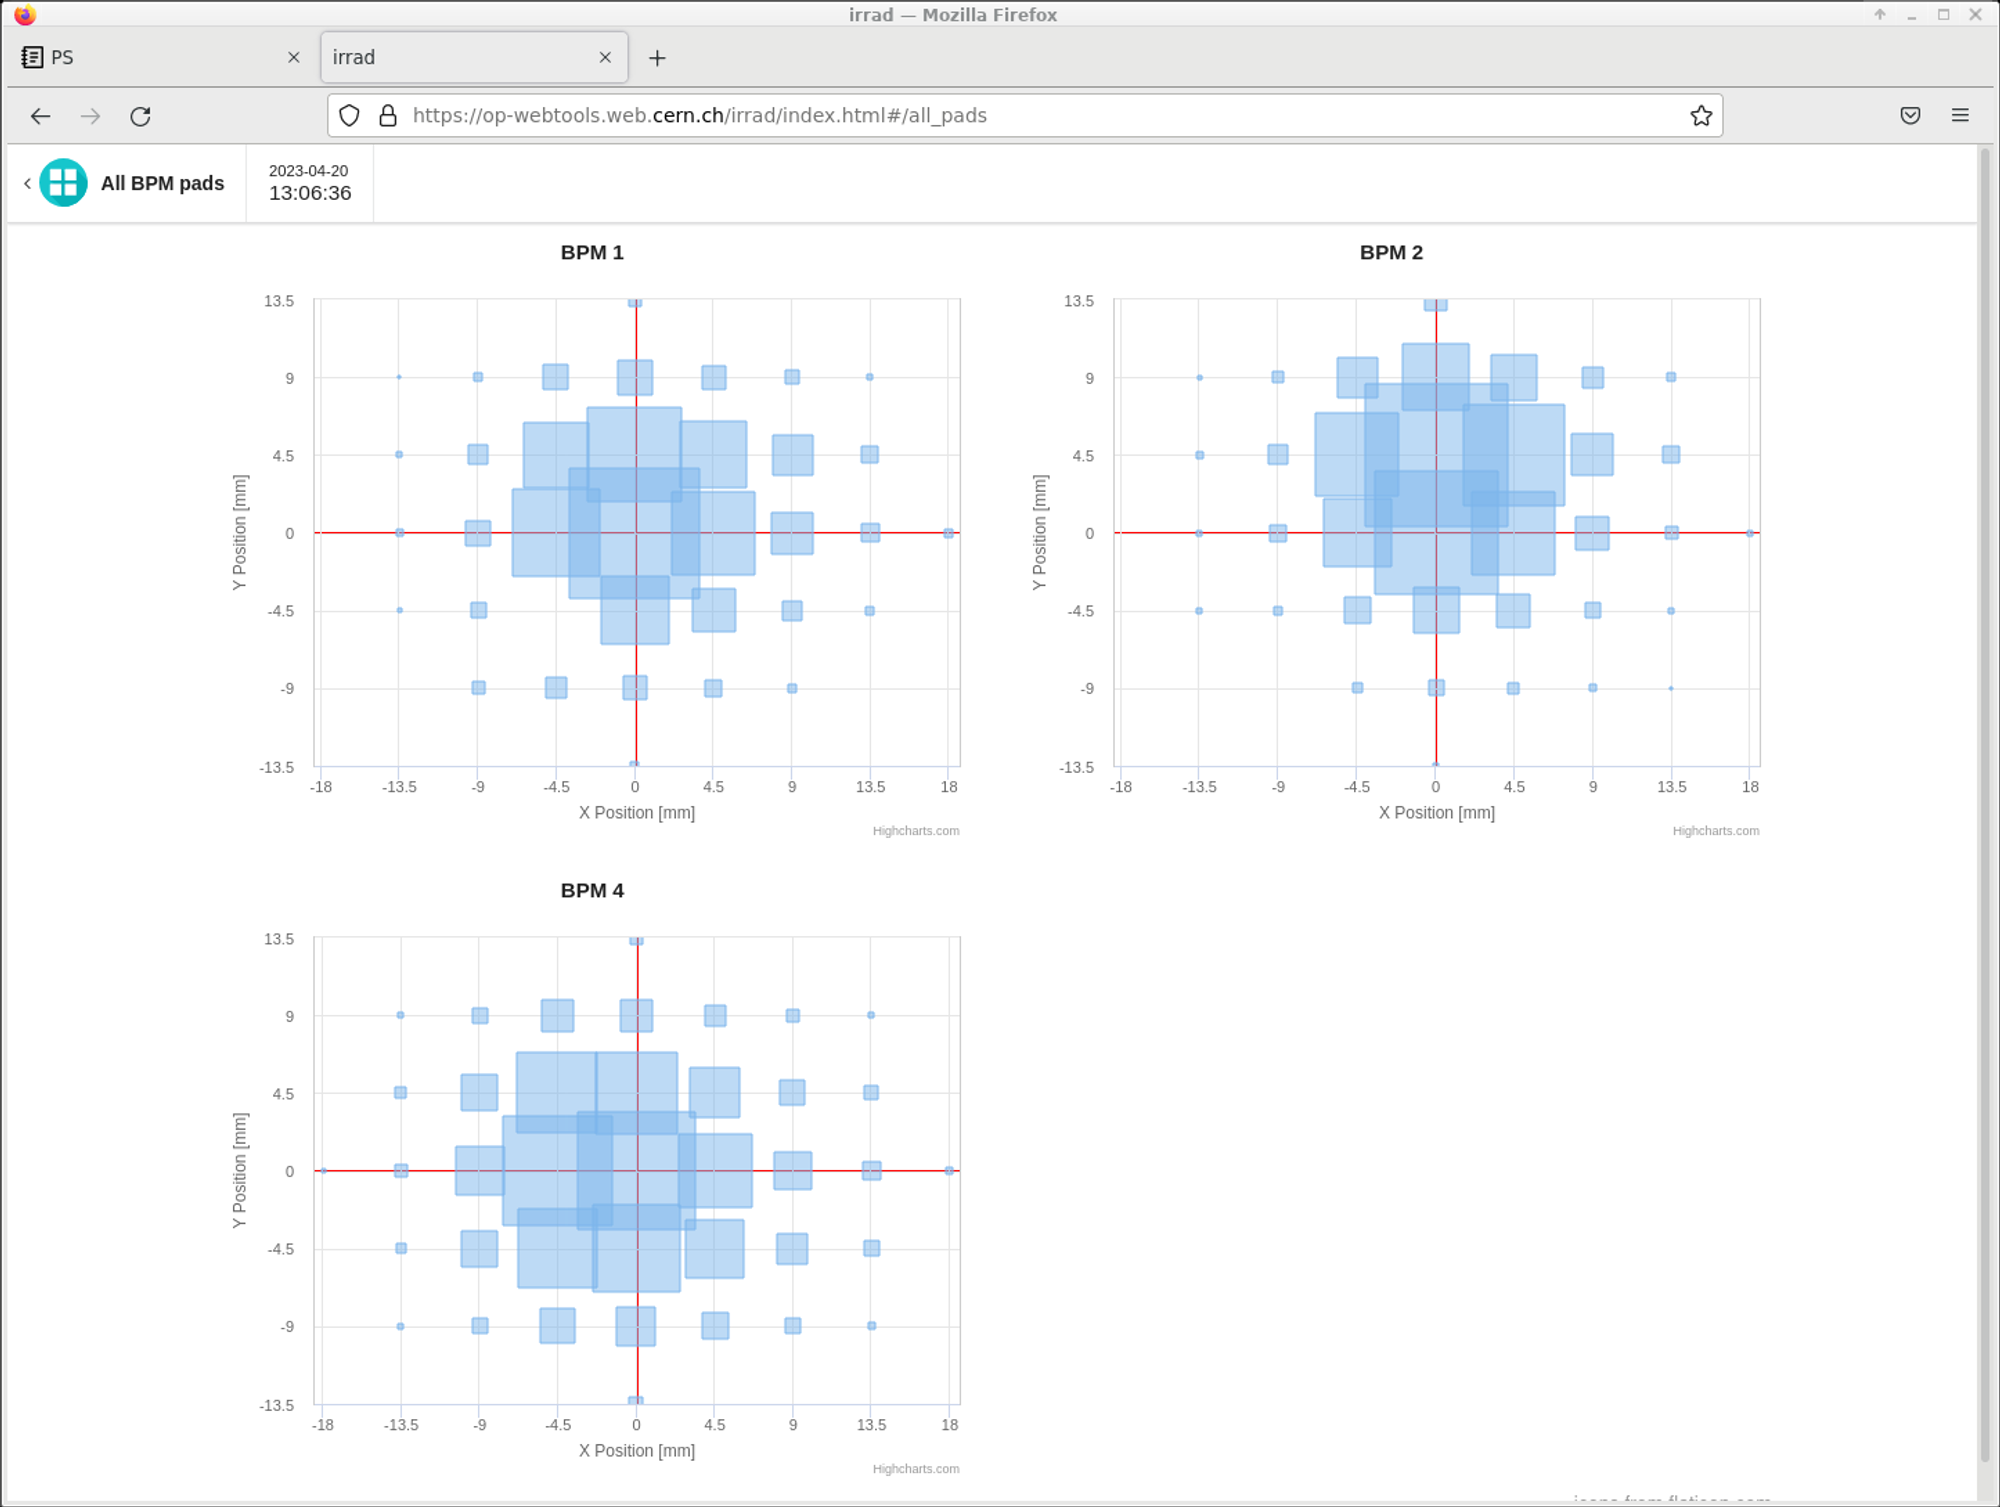
\includegraphics[width=1.0\textwidth]{03_Empirical_Measurements/images/irrad_new_optics.png}
% \caption{PTC simulation of the beam distribution in real space at the IRRAD BPMs location.}
% \label{fig:irrad_bpms_new_optics}
% \end{figure}

\subsection{Ion initial condition}

Reference to IPAC 2024 contribution.

%%%%%%%%%%%%%%%%%%%%%%%%%%%%%%%%%%%%%%%%%%%%%%%%%%%%%%%%%
%%%% Comparison between Simulation and  Measurements %%%%
%%%%%%%%%%%%%%%%%%%%%%%%%%%%%%%%%%%%%%%%%%%%%%%%%%%%%%%%%

\section{Compare initial parameters between simulation and empirical measurements}


%%%%%%%%%%%%%%%%%%%%%%%%%%%%%%%%
%%%%%% Conclusion %%%%%%%%%%%%%%
%%%%%%%%%%%%%%%%%%%%%%%%%%%%%%%%

\section{Conclusion}
This technical note has provided a comprehensive analysis of stray fields in the Proton Synchrotron (PS) at CERN, combining simulation and empirical measurements to understand their impact on beam dynamics. Using MAD-X and OPERA-3D simulation tools, we developed detailed magnetic models of the PS main units, revealing significant spatial variations in dipole and quadrupole fields due to combined-function magnets.

Empirical measurements, especially quadrupole scans at the East Dump, were crucial for validating these simulations. Advanced image processing techniques and the use of BTVs with filter wheels ensured precise beam size measurements, aiding in accurate determination of initial beam parameters.

Comparison between simulation and measurement highlighted discrepancies, particularly an underestimation of beam size in simulations, indicating potential unmodeled effects such as air scattering. Despite these differences, the study provided valuable insights into beam dynamics and stray field effects, contributing significantly to the understanding and management of stray fields in accelerator environments.

\bibliography{references.bib}
\bibliographystyle{IEEEtran}

\end{document}
